%  LaTeX support: latex@mdpi.com 
%  For support, please attach all files needed for compiling as well as the log file, and specify your operating system, LaTeX version, and LaTeX editor.

%=================================================================
\documentclass[diagnostics,article,accept,pdftex,moreauthors]{Definitions/mdpi} 
%\documentclass[preprints,article,submit,pdftex,moreauthors]{Definitions/mdpi} 
% For posting an early version of this manuscript as a preprint, you may use "preprints" as the journal. Changing "submit" to "accept" before posting will remove line numbers.
\usepackage{longtable} 
%--------------------
% Class Options:
%--------------------
%----------
% journal
%----------
% Choose between the following MDPI journals:
% accountaudit, acoustics, actuators, addictions, adhesives, adolescents, aerobiology, aerospace, agriculture, agriengineering, agrochemicals, agronomy, ai, aichem, aieng, aimater, aimed, aipa, air, aisens, algorithms, allergies, alloys, amh, analog, analytica, analytics, anatomia, anesthres, animals, antibiotics, antibodies, antioxidants, applbiosci, appliedchem, appliedmath, appliedphys, applmech, applmicrobiol, applnano, applsci, aquacj, architecture, arm, arthropoda, asc, asi, astronautics, astronomy, atmosphere, atoms, audiolres, automation, axioms, bacteria, batteries, bdcc, beverages, biochem, bioengineering, biologics, biology, biomass, biomechanics, biomed, biomedicines, biomedinformatics, biomimetics, biomolecules, biophysica, bioresourbioprod, biosensors, biosphere, biotech, birds, blockchains, bloods, blsf, brainsci, breath, buildings, cancers, carbon, cardio, cardiogenetics, cardiovascmed, catalysts, cells, ceramics, challenges, chemengineering, chemistry, chemosensors, chemproc, children, chips, cimb, civileng, cleantechnol, climate, clinbioenerg, clinpract, clockssleep, cmd, cmtr, coasts, coatings, colloids, colorants, commodities, complexities, complications, compounds, computation, computers, condensedmatter, conservation, constrmater, cosmetics, covid, crops, cryo, cryptography, crystals, csmf, ctn, culture, curroncol, cyber, dairy, data, ddc, dentistry, dermato, dermatopathology, designs, devices, dhi, diabetology, diagnostics, dietetics, digital, disabilities, diseases, diversity, dna, drones, dynamics, earth, ebj, ecm, ecologies, edm, eesp, electricity, electrochem, electronicmat, electronics, encyclopedia, endocrines, energies, eng, engproc, entomology, entropy, environments, environremediat, epidemiologia, epigenomes, esa, est, fermentation, fibers, fintech, fire, fishes, fluids, foods, forecasting, forensicsci, forests, fossstud, foundations, fractalfract, fuels, future, futureinternet, futurepharmacol, futurephys, futuretransp, galaxies, gases, gastroent, gastrointestdisord, gastronomy, gels, genes, geographies, geohazards, geomatics, geometry, geosciences, geotechnics, geriatrics, germs, glacies, grasses, green, greenhealth, gucdd, hardware, hazardousmatters, healthcare, hearts, hemato, hematolrep, hep, heritage, higheredu, highthroughput, horticulturae, hospitals, hydrobiology, hydrogen, hydrology, hydropower, hygiene, idr, iic, ijem, ijerph, ijgi, ijmd, ijms, ijns, ijom, ijpb, ijt, ijtm, ijtpp, ime, immuno, informatics, information, infrastructures, inorganics, insects, instruments, inventions, iot, j, jaestheticmed, jal, jcdd, jcm, jcp, jcrm, jcs, jcto, jdad, jdb, jdream, jemr, jeta, jfb, jfmk, jgbg, jgg, jimaging, jlpea, jmahp, jmmp, jmms, jmp, jmse, jne, jnt, jof, joi, joitmc, joma, jop, joptm, jor, jox, jpbi, jphytomed, jpm, jsan, jtaer, jvd, jzbg, kidneydial, kinasesphosphatases, knowledge, labmed, laboratories, lae, land, life, lights, limnolrev, lipidology, liquids, livers, logics, logistics, lubricants, lymphatics, machines, macromol, magnetism, magnetochemistry, make, marinedrugs, materials, materproc, mathematics, mca, measurements, medicina, medicines, medsci, membranes, merits, metabolites, metals, meteorology, methane, metrics, metrology, micro, microarrays, microbiolres, microelectronics, micromachines, microorganisms, microplastics, microwave, minerals, mining, mmphys, modelling, molbank, molecules, mps, msf, mti, multimedia, muscles, nanoenergyadv, nanomanufacturing, nanomaterials, ncrna, ndt, network, neuroglia, neuroimaging, neurolint, neurosci, nitrogen, notspecified, nursrep, nutraceuticals, nutrients, obesities, occuphealth, oceans, ohbm, onco, optics, oral, organics, organoids, osteology, oxygen, pandemics, parasites, parasitologia, particles, pathogens, pathophysiology, pediatrrep, pets, pharmaceuticals, pharmaceutics, pharmacoepidemiology, pharmacy, philosophies, photochem, photonics, phycology, physchem, physics, physiologia, plants, plasma, platforms, pollutants, polymers, polysaccharides, populations, poultry, powders, precipitation, precisoncol, preprints, proceedings, processes, prosthesis, proteomes, psf, psychiatryint, psychoactives, purification, quantumrep, quaternary, qubs, radiation, rdt, reactions, realestate, receptors, recycling, regeneration, remotesensing, reports, reprodmed, resources, rheumato, rjpm, robotics, rsee, ruminants, safety, sci, scipharm, sclerosis, seeds, sensors, separations, sexes, shi, signals, sinusitis, siuj, skins, smartcities, sna, societies, software, soilsystems, solar, solids, spectroscj, sports, standards, stats, std, stratsediment, stresses, surfaces, surgeries, suschem, sustainability, symmetry, synbio, systems, tae, targets, taxonomy, technologies, telecom, test, textiles, thalassrep, therapeutics, thermo, timespace, tomography, toxics, toxins, tph, transplantology, transportation, traumacare, traumas, tri, tropicalmed, universe, urbansci, uro, vaccines, vehicles, venereology, vetsci, vibration, virtualworlds, viruses, vision, waste, water, welding, wem, wevj, wild, wind, women, world, zoonoticdis

%---------
% article
%---------
% The default type of manuscript is "article", but can be replaced by: 
% abstract, addendum, article, benchmark, book, bookreview, briefcommunication, briefreport, casereport, changes, clinicopathologicalchallenge, comment, commentary, communication, conceptpaper, conferenceproceedings, correction, conferencereport, creative, datadescriptor, discussion, entry, expressionofconcern, extendedabstract, editorial, essay, erratum, fieldguide, hypothesis, interestingimages, letter, meetingreport, monograph, newbookreceived, obituary, opinion, proceedingpaper, projectreport, reply, retraction, review, perspective, protocol, shortnote, studyprotocol, supfile, systematicreview, technicalnote, viewpoint, guidelines, registeredreport, tutorial,  giantsinurology, urologyaroundtheworld
% supfile = supplementary materials

%----------
% submit
%----------
% The class option "submit" will be changed to "accept" by the Editorial Office when the paper is accepted. This will only make changes to the frontpage (e.g., the logo of the journal will get visible), the headings, and the copyright information. Also, line numbering will be removed. Journal info and pagination for accepted papers will also be assigned by the Editorial Office.

%------------------
% moreauthors
%------------------
% If there is only one author the class option oneauthor should be used. Otherwise use the class option moreauthors.

%---------
% pdftex
%---------
% The option pdftex is for use with pdfLaTeX. Remove "pdftex" for (1) compiling with LaTeX & dvi2pdf (if eps figures are used) or for (2) compiling with XeLaTeX.

%=================================================================
% MDPI internal commands - do not modify
\firstpage{1} 
\makeatletter 
\setcounter{page}{\@firstpage} 
\makeatother
\pubvolume{1}
\issuenum{1}
\articlenumber{0}
\pubyear{2026}
\copyrightyear{2026}
\externaleditor{Brett Lidbury} % More than 1 editor, please add `` and '' before the last editor name
\datereceived{30 April 2026} 
\daterevised{28 May 2026} % Comment out if no revised date
\dateaccepted{17 June 2026} 
\datepublished{6 July 2026} 
%\datecorrected{} % For corrected papers: "Corrected: XXX" date in the original paper.
%\dateretracted{} % For retracted papers: "Retracted: XXX" date in the original paper.
%\doinum{} % Used for some special journals, like molbank
%\pdfoutput=1 % Uncommented for upload to arXiv.org
%\CorrStatement{yes}  % For updates
%\longauthorlist{yes} % For many authors that exceed the left citation part
%\IsAssociation{yes} % For association journals

%=================================================================
% Add packages and commands here. The following packages are loaded in our class file: fontenc, inputenc, calc, indentfirst, fancyhdr, graphicx, epstopdf, lastpage, ifthen, float, amsmath, amssymb, lineno, setspace, enumitem, mathpazo, booktabs, titlesec, etoolbox, tabto, xcolor, colortbl, soul, multirow, microtype, tikz, totcount, changepage, attrib, upgreek, array, tabularx, pbox, ragged2e, tocloft, marginnote, marginfix, enotez, amsthm, natbib, hyperref, cleveref, scrextend, url, geometry, newfloat, caption, draftwatermark, seqsplit
% cleveref: load \crefname definitions after \begin{document}

\usepackage[nolist]{acronym}        % For managing acronyms (as specified)
\usepackage{numprint}       % For number formatting (as specified)
%\usepackage{subcaption}     % For subfigures (as specified)
\usepackage{longtable}      % For multi-page tables
\usepackage{multirow}       % For cells spanning multiple rows
% \usepackage{ltablex}
% \keepXColumns
\usepackage{subfig}
\usepackage{algorithm}      % For algorithm environments
\usepackage{algpseudocode}  % For pseudocode formatting
\usepackage{listings}       % For source code listings
\usepackage{siunitx}        % For SI unit formatting
\usepackage{bm}             % For bold math symbols
\usepackage{mathtools}      % Extends amsmath with additional features
% for drawing with tikz
\usepackage{tikz}

\usetikzlibrary{calc}
\usetikzlibrary{arrows.meta,positioning,shapes.geometric,fit,backgrounds}
% Track changes for reviewer revisions (remove before final submission)
% Usage: new text  
%% [DELETED R2]: old text  new
%% [OLD R1]: old
% To produce final clean copy: % \usepackage[final]{changes}  % stripped by make-final.py
% \usepackage[final]{changes}  % stripped by make-final.py
% % stripped by make-final.py % uncomment to show marks for reviewers
% \definechangesauthor[name={Reviewer~1},color=blue]{R1}
% \definechangesauthor[name={Reviewer~2},color=teal]{R2}
% \definechangesauthor[name={Reviewers~1\&2},color=violet]{R12}
%=================================================================
% Please use the following mathematics environments: Theorem, Lemma, Corollary, Proposition, Characterization, Property, Problem, Example, ExamplesandDefinitions, Hypothesis, Remark, Definition, Notation, Assumption
%% For proofs, please use the proof environment (the amsthm package is loaded by the MDPI class).

%=================================================================
% Full title of the paper (Capitalized)
\Title{A Machine Learning Framework for Preeclampsia Prediction at
  Isidro Ayora Hospital, Ecuador}
% Previous title: Preeclampsia Prediction at Isidro Ayora Hospital (ECU) using Machine Learning

% Author Orchid ID: enter ID or remove command
% \newcommand{\orcidauthorA}{0000-0000-0000-000X} % Add \orcidA{}
% behind the author's name

\newcommand{\orcidauthorA}{0000-0003-0942-673X} % María Pérez
\newcommand{\orcidauthorB}{0000-0003-4402-6643} % Lenin Falconí
\newcommand{\orcidauthorC}{0000-0002-8390-3269} % Monserrate Intriago
\newcommand{\orcidauthorD}{0000-0001-8648-7865} % Andrés Bastidas-Fuertes
\newcommand{\orcidauthorE}{0000-0003-4527-7137} % Juan Benavidez
\newcommand{\orcidauthorF}{0000-0003-0064-7528} % Raysa A. Fuertes-Arévalo

%\newcommand{\orcidauthorB}{0000-0000-0000-000X} % Add \orcidB{} behind the author's name

% Authors, for the paper (add full first names)
\Author{{Maria Perez} %MDPI: Please carefully check the accuracy of names and affiliations.
 $^{1,}$*\orcidA{}, Lenin G. Falconi $^{1}$\orcidB{},
  Monserrate Intriago-Pazmiño $^{1}$\orcidC{}, Andrés Bastidas-Fuertes $^{2}$\orcidD{}, Juan~Benavides~$^{1}$\orcidE{} and Raysa A. Fuertes-Arévalo $^{3}$\orcidF{}}

%\longauthorlist{yes}

% MDPI internal command: Authors, for metadata in PDF
\AuthorNames{Maria Perez, Lenin G. Falconi, Monserrate
  Intriago-Pazmiño, Andrés Bastidas-Fuertes, Juan Benavides, and Raysa A. Fuertes-Arévalo}

% Affiliations / Addresses (Add [1] after \address if there is only one affiliation.)
\address{%
$^{1}$ \quad Departamento de Informática y Ciencias de la Computación,
Escuela Politécnica Nacional,  \mbox{Quito 170525, Ecuador;}
maria.perez@epn.edu.ec~(M.P.); lenin.falconi@epn.edu.ec~(L.G.F.); monserrate.intriago@epn.edu.ec~(M.I.-P.); 
juan.benavides@epn.edu.ec~(J.B.)\\ %<<AUTHOR: maria.perez email added>>
$^{2}$ \quad Smartwork S.A.,  {Quito 170503, Ecuador;} %MDPI: Newly
                                %added  information. Please
                                %confirm. <<AUTHOR: Confirmed!>>
 andres.bastidas@smartwork.com.ec~(A.B.-F.)\\ % <<AUTHOR: acronym added>>
$^{3}$ \quad Ministerio de Salud Pública, {Quito 170702,}
% MDPI: Please add the postal code. If a postal code is not available,
% a Post Office Box number can be added instead. <<AUTHOR:Added.>>
 Ecuador; raysafuertesa@gmail.com~(R.A.F.-A.c)} %<<AUTHOR: acronym added>>

% Contact information of the corresponding author
% \corres{Correspondence: e-mail@e-mail.com; Tel.: (optional; include
% country code; if there are multiple corresponding authors, add
% author initials) +xx-xxxx-xxx-xxxx (F.L.)}

\corres{Correspondence: maria.perez@epn.edu.ec}

% Current address and/or shared authorship
%\firstnote{Current address: Affiliation.}  
% Current address should not be the same as any items in the Affiliation section.

%\secondnote{These authors contributed equally to this work.}
% The commands \thirdnote{} till \eighthnote{} are available for further notes.

%\simplesumm{} % Simple summary

%\conference{} % An extended version of a conference paper

% Abstract (Do not insert blank lines, i.e., \\) 
% \abstract{A single paragraph of about 200 words maximum. For
% research articles, abstracts should give a pertinent overview of the
% work. We strongly encourage authors to use the following style of
% structured abstracts, but without headings: (1) Background: place
% the question addressed in a broad context and highlight the purpose
% of the study; (2) Methods: describe briefly the main methods or
% treatments applied; (3) Results: summarize the article's main
% findings; (4) Conclusions: indicate the main conclusions or
% interpretations. The abstract should be an objective representation
% of the article, it must not contain results which are not presented
% and substantiated in the main text and should not exaggerate the
% main conclusions.}

% \abstract{\textbf{Background:} Preeclampsia is a major contributor to
%   maternal and perinatal morbidity. In Ecuadorian public hospitals,
%   clinical information is often fragmented, limiting the construction
%   of complete datasets for prediction modeling. \textbf{Methods:} This
%   study aimed to develop a machine learning model to predict
%   preeclampsia using demographic data from the Isidro Ayora Hospital
%   in Quito, Ecuador. We proposed a custom automated machine learning
%   (C-AutoML) workflow to evaluate six models (Logistic Regression,
%   LightGBM, XGBoost, CatBoost, Multi-Layer Perceptron, and Random
%   Forest) and compared its performance to a weighted ensemble built
%   using AWS SageMaker Canvas, optimizing for the F1-score. Model
%   interpretability was analyzed using \ac{SHAP}. Due to the scarcity
%   of clinical variables, a synthetic dataset based on FullPIERS
%   predictors was also generated and modeled. \textbf{Results:} On the
%   hospital dataset, the SageMaker ensemble achieved an F1-score of
%   0.805, accuracy of 0.934, and AUC of 0.956, while the C-AutoML's
%   best single model (LightGBM) achieved comparable results (F1-score:
%   0.802, accuracy: 0.938, AUC: 0.944). \ac{SHAP} analysis identified
%   patient age as the most influential feature. On the synthetic
%   dataset, Logistic Regression achieved perfect performance (F1-score:
%   1.0). \textbf{Conclusions:} The proposed C-AutoML workflow matched
%   the performance o the weighted ensemble model trained in AWS using a
%   single, model. Despite the current reliance on
%   demographic data, the methodology shows promise for aiding
%   preeclampsia diagnosis in resource-limited settings, with future
%   integration of clinical data expected to enhance predictive power
%   for risk assessment.}

% \abstract{Preeclampsia is a major contributor to maternal and
%   perinatal morbidity. In Ecuadorian public hospitals, clinical
%   information is often fragmented, limiting the construction of
%   complete datasets for prediction modeling. This study aimed to
%   develop a machine learning model to predict preeclampsia using
%   demographic data from the Isidro Ayora Hospital (HGIO), Quito,
%   Ecuador. We proposed a custom automated machine learning (C-AutoML)
%   workflow to evaluate six models (Logistic Regression, LightGBM,
%   XGBoost, CatBoost, Multi-Layer Perceptron, and Random Forest) and
%   compared its performance to a weighted ensemble built using AWS
%   SageMaker Canvas, optimizing for the F1-score in both cases. Model
%   interpretability was analyzed using \ac{SHAP}. Due to the scarcity
%   of clinical variables, a synthetic dataset based on FullPIERS
%   predictors was also generated and modeled. On the hospital dataset,
%   the SageMaker ensemble achieved an F1-score of 0.805, accuracy of
%   0.934, and AUC of 0.956, while the C-AutoML's best single model
%   (LightGBM) achieved comparable results (F1-score: 0.802, accuracy:
%   0.938, AUC: 0.944). \ac{SHAP} analysis identified patient age as the
%   most influential feature. On the synthetic dataset, Logistic
%   Regression achieved perfect performance (F1-score: 1.0). As a
%   result, the proposed C-AutoML workflow matched the performance of a
%   the weighted ensemble tool using a single, interpretable
%   model. Despite the current reliance on demographic data, the
%   methodology shows promise for aiding preeclampsia diagnosis in
%   resource-limited settings, with future integration of clinical data
%   expected to enhance predictive power for risk assessment.}

\abstract{\textbf{Background:} Preeclampsia (PE) is a leading cause
  of maternal and perinatal morbidity, affecting 2--8\% of pregnancies
  worldwide. In Ecuadorian public hospitals, clinical data are often
  fragmented, limiting the construction of complete datasets for
  prediction modeling. This study aimed to develop a Machine Learning
  (ML) framework to predict PE using demographic data from the Isidro
  Ayora Gynecology and Obstetrics Hospital (HGOIA), Quito, Ecuador.
  \textbf{Methods:} We proposed a custom automated Machine Learning
  (C-AutoML) workflow to evaluate six models (Logistic Regression,
  LightGBM, XGBoost, CatBoost, Multi-Layer
  Perceptron, and Random Forest) and compared its performance against
  a weighted ensemble built with Amazon SageMaker Canvas, optimizing for
  the F1-score. Model interpretability was analyzed using Shapley
  Additive Explanations (SHAP). Due to the scarcity of clinical
  variables at HGOIA, a synthetic dataset based on FullPIERS predictors
  was also generated and modeled.
  \textbf{Results:} On the hospital dataset, the SageMaker ensemble
  achieved an F1-score of 0.805, accuracy of 0.934, and AUC of 0.956,
  while the C-AutoML best single model (LightGBM) yielded
  comparable results (F1-score: 0.802, accuracy: 0.938, AUC: 0.944).
  SHAP analysis identified patient age as the most influential
  feature. On the synthetic dataset, Logistic Regression achieved
  perfect classification \mbox{(F1-score: 1.0).}
  \textbf{Conclusions:} The proposed C-AutoML framework matched the
  performance of the SageMaker weighted ensemble while relying on a
  single, interpretable model. Despite the current dependence on
  demographic data, the methodology shows promise for supporting PE
  diagnosis in resource-limited settings; future integration of
  clinical variables is expected to further enhance predictive power
  for risk stratification.}

% Keywords 3 to 10
\keyword{machine learning; explainable artificial intelligence;
  preeclampsia; prediction; LightGBM; ensemble models } 

% The fields PACS, MSC, and JEL may be left empty or commented out if not applicable
%\PACS{J0101}
%\MSC{}
%\JEL{}

%%%%%%%%%%%%%%%%%%%%%%%%%%%%%%%%%%%%%%%%%%
% Only for the journal Diversity
%\LSID{\url{http://}}

%%%%%%%%%%%%%%%%%%%%%%%%%%%%%%%%%%%%%%%%%%
% Only for the journal Applied Sciences
%\featuredapplication{Authors are encouraged to provide a concise description of the specific application or a potential application of the work. This section is not mandatory.}
%%%%%%%%%%%%%%%%%%%%%%%%%%%%%%%%%%%%%%%%%%

%%%%%%%%%%%%%%%%%%%%%%%%%%%%%%%%%%%%%%%%%%
% Only for the journal Data
%\dataset{DOI number or link to the deposited data set if the data set is published separately. If the data set shall be published as a supplement to this paper, this field will be filled by the journal editors. In this case, please submit the data set as a supplement.}
%\datasetlicense{License under which the data set is made available (CC0, CC-BY, CC-BY-SA, CC-BY-NC, etc.)}

%%%%%%%%%%%%%%%%%%%%%%%%%%%%%%%%%%%%%%%%%%
% Only for the journal BioTech, Fishes, Neuroimaging and Toxins
%\keycontribution{The breakthroughs or highlights of the manuscript. Authors can write one or two sentences to describe the most important part of the paper.}

%%%%%%%%%%%%%%%%%%%%%%%%%%%%%%%%%%%%%%%%%%
% Only for the journal Encyclopedia
%\encyclopediadef{For entry manuscripts only: please provide a brief overview of the entry title instead of an abstract.}

%%%%%%%%%%%%%%%%%%%%%%%%%%%%%%%%%%%%%%%%%%
% Different journals have different requirements. Please check the specific journal guidelines in the "Instructions for Authors" on the journal's official website.
%\addhighlights{yes}
%\renewcommand{\addhighlights}{%
%
%\noindent The goal is to increase the discoverability and readability of the article via search engines and other scholars. Highlights should not be a copy of the abstract, but a simple text allowing the reader to quickly and simplified find out what the article is about and what can be cited from it. Each of these parts should be devoted up to 2~bullet points.\vspace{3pt}\\
%\textbf{What are the main findings?}
% \begin{itemize}[labelsep=2.5mm,topsep=-3pt]
% \item First bullet.
% \item Second bullet.
% \end{itemize}\vspace{3pt}
%\textbf{What are the implications of the main findings?}
% \begin{itemize}[labelsep=2.5mm,topsep=-3pt]
% \item First bullet.
% \item Second bullet.
% \end{itemize}
%}

%%%%%%%%%%%%%%%%%%%%%%%%%%%%%%%%%%%%%%%%%%
\begin{document}
% Acronyms
\begin{acronym}
    \acro{PE}[PE]{Preeclampsia}
    \acro{HDP}[HDP]{Hypertensive Disorders of Pregnancy}
    \acro{HPO}[HPO]{Hyperparameter Optimization}
    \acro{ML}[ML]{Machine Learning}
    \acro{SHAP}[SHAP]{SHapley Additive exPlanations}
    \acro{BMI}[BMI]{Body Mass Index}
    \acro{AUC}[AUC]{Area Under the Receiver Operating Characteristic Curve}
    \acro{F1}[F1]{F1-score}
    \acro{MSP}[MSP]{Ministerio de Salud Pública}
    \acro{PUCE}[PUCE]{Pontifical Catholic University of Ecuador}
    %\acro{ANN}[ANN]{Artificial Neural Network} % unused in body text
    \acro{MLOPs}[MLOPs]{Machine Learning Operations}
    \acro{PIERS}[PIERS]{Preeclampsia Integrated Estimate of RiSk}
    \acro{ICD-10}[ICD-10]{International Classification of Diseases}
    \acro{ACC}[ACC]{Accuracy}
    \acro{C-AutoML}[C-AutoML]{Custom Automated Machine
      Learning Workflow}
    \acro{MLP}[MLP]{Multi-Layer Perceptron}
    \acro{LR}[LR]{Logistic Regression}
    \acro{RF}[RF]{Random Forest}
    \acro{SVM}[SVM]{Support Vector Machine}
    \acro{EN}[EN]{Elastic Net Logistic Regression}
    \acro{w.r.t.}[w.r.t.]{with respect to}
    \acro{HTN}[HTN]{Hypertension}
    \acro{SBP}[SBP]{Systolic Blood Pressure}
    \acro{DBP}[DBP]{Diastolic Blood Pressure}
    \acro{ULN}[ULN]{Upper Limit of Normal}
    \acro{GA}[GA]{Gestational Age}
    \acro{AST}[AST]{Aspartate Aminotransferase}
    \acro{WHO}[WHO]{World Health Organization}
    \acro{HGOIA}[HGOIA]{Isidro Ayora Gynecology and Obstetrics Hospital}
    \acro{EPN}[EPN]{Escuela Politécnica Nacional}
    \acro{API}[API]{Application Programming Interface}
    \acro{EHR}[EHR]{Electronic Health Records}
\end{acronym}
  
  
%%%%%%%%%%%%%%%%%%%%%%%%%%%%%%%%%%%%%%%%%%
% \setcounter{section}{-1} %% Remove this when starting to work on the template.
% \section{How to Use this Template}

% The template details the sections that can be used in a manuscript. Note that the order and names of article sections may differ from the requirements of the journal (e.g., the positioning of the Materials and Methods section). Please check the instructions on the authors' page of the journal to verify the correct order and names. For any questions, please contact the editorial office of the journal or support@mdpi.com. For LaTeX-related questions please contact latex@mdpi.com.%\endnote{This is an endnote.} % To use endnotes, please un-comment \printendnotes below (before References). Only journal Laws uses \footnote.

% % The order of the section titles is different for some journals. Please refer to the "Instructions for Authors” on the journal homepage.

\section{Introduction}
\label{sec:introduction}
\Ac{PE}, a leading hypertensive disorder of pregnancy, is
a major cause of maternal and perinatal morbidity and mortality
worldwide, being associated with more than {70,000}
maternal deaths and over {500,000} fetal and neonatal deaths
annually~\cite{vera2025preeclampsia}. The \ac{WHO} reports that \ac{PE}
affects approximately 2--8\% of pregnancies globally, with
a pooled global prevalence estimated at 4.43\%~\cite{vera2025preeclampsia},
highlighting the relevance of early detection and risk stratification
strategies~\cite{who_2025_preeclampsia,vera2025preeclampsia}.

Clinically, \ac{PE} is a complex multisystem disorder
defined as new-onset hypertension (\ac{SBP} $\geq$ 140~mmHg or
\ac{DBP} $\geq$ 90~mmHg) after 20 weeks of gestation in previously
normotensive women, accompanied by at least one of: proteinuria,
evidence of maternal end-organ dysfunction, or signs of uteroplacental
insufficiency such as fetal growth restriction. This departs from earlier
criteria that required proteinuria in all
cases~\cite{brown2018isshp,vera2025preeclampsia}. The condition is
multifactorial in origin, with key risk factors including advanced
maternal age, obesity, chronic hypertension, diabetes, and limited
access to prenatal care~\cite{vera2025preeclampsia}. Although \ac{PE}
typically develops in the second half of pregnancy, clinical onset can
occur for the first time during labor or within the early postpartum
period, as the underlying vascular dysregulation does not resolve
immediately at delivery~\cite{brown2018isshp}.
International guidelines further distinguish early-onset \ac{PE} (onset
before 34 weeks of gestation) from late-onset \ac{PE} (at or after 34
weeks), which differ in placental pathophysiology, severity profile, and
associated neonatal morbidity~\cite{brown2018isshp}. Contemporary
practice discourages classifying cases into separate mild and severe
forms, as even apparently moderate presentations may progress abruptly
to life-threatening complications; presentations accompanied by markedly
elevated blood pressures, thrombocytopenia, renal insufficiency, hepatic
dysfunction, pulmonary edema, or new-onset headache are instead
characterized as having severe features, requiring urgent
management~\cite{brown2018isshp}. Collectively, these features underscore
the clinical complexity of \ac{PE} and the need for robust,
population-adapted analytic strategies to support timely identification
of at-risk pregnancies~\cite{vera2025preeclampsia}.

In Ecuador, the Clinical Practice Guideline from the
\ac{MSP}~{(Ministry of Public Health)} %MDPI: Footnotes are not
                                %supported in our journal. We have
                                %therefore included this paragraph in
                                %the main text. Please confirm. Same
                                %with whole tex file. <<AUTHORS: Agree>>
 identifies
\ac{PE} and eclampsia among the principal causes of maternal
death. It reports that these conditions were the leading cause of
maternal mortality, accounting for 27.53\% of maternal deaths from
2006 to 2014~\cite{msp_ecuador_hdp_2013}. This epidemiological burden
supports the need for local analytic approaches that characterize risk
patterns in hospital populations and can inform timely referral and
surveillance.

% improve with prism
In recent years, \ac{ML} has been increasingly applied to \ac{PE}
prediction, with studies showing promising discriminatory performance
using routinely collected variables~\cite{LI2021102,mennickent_2023,Darsareh2024,Rahman2023}.
These approaches identify non-linear risk patterns from maternal
characteristics, vital signs, laboratory measurements, and obstetric
history, enabling earlier and more individualized risk estimation than
rule-based screening alone~\cite{LI2021102,mennickent_2023}. Clinically,
this is important for proactive surveillance, prioritization of
high-risk pregnancies, and more efficient allocation of limited
healthcare resources, particularly in high-volume settings with
heterogeneous data quality.

The full \ac{PIERS} model estimates the probabilistic
risk of adverse maternal outcomes in women with \ac{PE} {using}
% <<AUTHOR: introducing gestational age acronym>>
\ac{GA}, chest pain or dyspnoea, oxygen saturation
({$\text{SpO}_2$}), creatinine, platelet count, and aspartate transaminase
(\ac{AST}), including quadratic and interaction terms, as
predictors~\cite{fullpiers_2011}. It uses the Logistic Regression
equation in~\eqref{eq:logistic-regression}, where the logit is
calculated as a linear combination of these variables as depicted
in~\eqref{eq:fullpiers-logit} and the coefficient values are those
{proposed} %MDPI: Please ensure all variables/values in the equation appear in the same format in the text (normal/italic/bold/subscript/superscript).
 in~\cite{fullpiers_2011}.
%<<AUTHORS: Confirmed. We standardised the typographic format of all variables: (1) the function name ``logit'' now uses \text{logit} (upright Roman) consistently in both Eq.~1 and Eq.~2; (2) the variable SpO\textsubscript{2} in the surrounding text was updated to $\text{SpO}_2$ matching the equation style; (3) the spelling ``dyspnoea'' was unified to the British form used in the equation. All other variable names (gestational age, chest pain, creatinine, platelets, aspartate transaminase, AST) were already rendered uniformly with \text{} throughout.>>
%% [OLD R2]: The full\ac{PIERS} model uses demographic and laboratory variables
%% (e.g., gestational age, creatinine, platelet count, aspartate
%% transaminase, etc.) to estimate the probabilistic risk of adverse
%% maternal outcomes among women with
%% \ac{PE}~\cite{fullpiers_2011}. It uses the logistic regression
%% equation in~\eqref{eq:logistic-regression}, where the logit is
%% calculated as a linear combination of variables
%% as depicted in~\eqref{eq:fullpiers-logit} and the coefficient values
%% are those proposed in~\cite{fullpiers_2011}. 
\begin{linenomath}
\begin{equation}
  \text{Probability Risk}(\text{logit})=1/(1+\exp^{-\text{logit}})
  \label{eq:logistic-regression}
\end{equation}
\end{linenomath}
\begin{linenomath}
\begin{equation}
  \begin{aligned}
    \text{logit}(\pi) &= 2.68 \\ %<<AUTHORS: Changed \texttt{logit} to \text{logit} to match the upright Roman style used for the same function name in Eq.~1, ensuring consistent variable/value formatting across both equations as requested.>>
              &\quad + (-5.41 \times 10^{-2} \times \text{gestational age at eligibility}) \\
              &\quad + (1.23 \times \text{chest pain or dyspnoea}) \\
              &\quad + (-2.71 \times 10^{-2} \times \text{creatinine}) \\
              &\quad + (2.07 \times 10^{-1} \times \text{platelets}) \\
              &\quad + (4.00 \times 10^{-5} \times \text{platelets}^2) \\
              &\quad + (1.01 \times 10^{-2} \times \text{aspartate transaminase}) \\
              &\quad + (-3.05 \times 10^{-6} \times \text{AST}^2) \\
              &\quad + (2.5 \times 10^{-4} \times \text{creatinine} \times \text{platelet}) \\
              &\quad + (-6.99 \times 10^{-5} \times \text{platelet} \times \text{aspartate transaminase}) \\
              &\quad + (-2.56 \times 10^{-3} \times \text{platelet} \times \text{SpO}_2)
  \end{aligned}
    \label{eq:fullpiers-logit}
\end{equation}
\end{linenomath}

However, a major operational challenge for \ac{EHR} in Ecuador
is the fragmentation of clinical information systems. In many
hospitals linked to the \ac{MSP}, complementary examinations are
recorded in separate databases or remain only in paper-based formats,
which limits immediate construction of complete and standardized
electronic clinical datasets for modeling. As a consequence, in this
research, we used the provided records from the
\ac{HGOIA}~({{Hospital Gineco Obstétrico Isidro Ayora (HGOIA),}
  % MDPI: Please confirm if the italics are necessary; if not, please
  % remove them. Same with all italic in tex file <<AUTHORS: italics were removed>>
 a
  third-level public specialty hospital in Zone~9 of the \ac{MSP},
  Quito, Ecuador}), which contains demographic variables and lacks
clinical features. For this reason, we explored our sets of models
both on the \ac{HGOIA} and synthetic datasets to diagnose
\ac{PE}. The synthetic dataset was constructed using the
full\ac{PIERS} equation~\eqref{eq:fullpiers-logit} as the
reference framework for feature distributions and the
\ac{MSP} clinical guideline~\cite{msp_ecuador_hdp_2013} for
the diagnostic label (Section~\ref{sec:synth-data-gener}). Unlike the full\ac{PIERS} standard, which is a
prognostic model, our goal is to determine the most effective set of
models to diagnose \ac{PE} according to the Ecuadorian realm.

In this work, we propose a custom automated Machine Learning workflow
that explores up to six classification algorithms
(\ac{LR}~\cite{cox1958logistic}, LightGBM~\cite{ke2017lightgbm},
XGBoost~\cite{chen2016xgboost},
CatBoost~\cite{prokhorenkova2018catboost}, 
\ac{MLP} \cite{rumelhart1986backprop}, and
\ac{RF}~\cite{breiman2001randomforest}) as candidate models for
\ac{PE} diagnostic prediction. Amazon SageMaker was also used to
evaluate the predictive power of the demographic variables of the
dataset of patients at \ac{HGOIA} and to train a reference
classifier. To improve classification, given the imbalanced data, we
target the \ac{F1} metric to balance sensitivity and precision. Our
results show that an ensemble model formed by LightGBM, \ac{RF} and
\ac{MLP} achieves \ac{F1} of 0.805, outperforming single models. To
provide interpretability for our model and avoid its use as a
black-box, we employed \ac{SHAP} to quantify the contribution of each
feature to the model's predictions. Patient age is the most
influential feature followed by {the} \ac{GA} % <<AUTHOR: using
% gestational age acronym instead>>
in weeks. Finally, to account for the lack of clinical data records,
we explored the same models with a synthetic dataset of our own.

The contributions of our work are as follows: (i) to the best of our knowledge,
this is the first study to address the use of machine
learning algorithms in \ac{PE} in Ecuador, (ii) we systematically
explored different Machine Learning models aiming to improve
classification performance as well as model's explainability, (iii) we
used data provided from \ac{HGOIA}, a specialized
public health facility in gynecology and obstetrics, (iv) we explored
additional models on synthetic data to account for lack of clinical
variables, (v) we deployed our model using a Machine Learning Operation (MLOP) approach in a
server at \ac{EPN}, including a web-based inference interface (see
Appendix~\ref{app:mlops-interface}).

\section{Related Works}
\label{sec:related-works}
Recent literature shows sustained interest in using \ac{ML} for
\ac{PE} prediction, but also highlights important differences in
study design, data sources, and intended clinical use. Two recent
systematic reviews synthesize this landscape. Darsareh et
al.~\cite{Darsareh2024} reviewed \ac{ML}-based prediction studies and
reported that the best-performing approaches commonly included elastic
net, stochastic gradient boosting, extreme gradient boosting, and
Random Forest, with \ac{AUC} values ranging approximately from 0.860 to
0.973. Similarly, Rahman et al.~\cite{Rahman2023} surveyed studies
published between 2018 and 2022 and concluded that \ac{ML} was the
dominant analytical paradigm in this domain, with ensemble and
boosting methods frequently achieving the highest predictive
performance. Their review also shows that demographic variables were
used much more frequently than laboratory variables among the sampled
papers, with demographic features representing 53\% of the reviewed
inputs versus only 15\% for laboratory data~\cite{Rahman2023}. This
observation is relevant in our context, given the type of variables
gathered from \ac{HGOIA} for our study. However, we
disagree with their model ranking, which primarily emphasizes
accuracy, because from a clinical point of view, overlooking high-risk
pregnancies is more consequential than accepting a moderate increase
in false positives. Hence, we consider the ranking should be on the
\ac{F1} or recall metrics, since a higher value in recall, reduces the
false negatives.

Beyond systematic reviews, several primary studies illustrate the
diversity of \ac{PE} prediction strategies. Marin et
al.~\cite{marin2019} used the Viterbi algorithm to determine the
presence of \ac{PE} based on features such as the weight, age,
and blood-pressure measurements. Their approach was integrated with a
smart bracelet and a mobile application to monitor the evolution of
the physiological parameters. This showed potential to be used in
hospitals as well as in remote monitoring of patients for early
detection of the condition. Li et al.~\cite{LI2021102} explored
\ac{LR}, \ac{RF}, Support Vector Machines (SVMs), and XGBoost models to predict women at
risk of \ac{PE} from Electronic Health Records collected in early
pregnancy. The XGBoost model achieved the best performance
($\mathrm{ACC}=0.920$, $\mathrm{Precision}=0.447$, $\mathrm{Recall}=0.789$,
$\mathrm{F1}=0.571$, $\mathrm{AUC}=0.955$) and showed that routinely available
structured clinical variables combining maternal factors and
laboratory data, such as fasting plasma glucose, mean blood pressure,
and \ac{BMI}, can provide useful discriminative power for \ac{PE}
risk prediction. Mari\'{c} et al.~\cite{mari__2022} used \ac{EN} with
stacked multiomics integration on longitudinal data from a small
prospective pregnancy cohort and achieved early prediction of
\ac{PE} ($\mathrm{AUC}=0.83$) using a 9‑metabolite urine model, with
performance improving to $\mathrm{AUC}=0.94$ when integrating multiple
omics modalities, demonstrating that molecular features are strong
contributors to predictive performance because they capture
pathophysiological processes before symptom onset and change earlier
than traditional clinical signs; clinical variables were predictive
but secondary and complementary, providing less information than
omics‑derived biomarkers.

Taken together, prior work suggests three major trends. First,
\ac{PE} prediction models tend to perform best when they combine
multiple domains of information, including maternal history,
hemodynamic measurements, laboratory values, and sometimes ultrasound
or omics data~\cite{Darsareh2024,Rahman2023,mennickent_2023}. Second,
tree-based ensembles and boosting algorithms are frequently reported
as top performers, although simpler models such as logistic
regression or elastic net can remain competitive when predictors are
well structured and clinically meaningful~\cite{Darsareh2024,LI2021102,mari__2020}.
Third, despite strong reported predictive metrics, many studies
were developed in data-rich environments and depend on comprehensive
electronic records that may not be available in middle-income public
hospital settings.

Our study is positioned within this literature but addresses a
different operational context. Instead of assuming a mature,
fully integrated electronic clinical infrastructure, we combine: (i)
a descriptive analysis of retrospective patient records from \ac{HGOIA}, (ii) a cloud-managed benchmarking workflow, and (iii) a
custom automated \ac{ML} pipeline with explainability analysis. In
addition, because fragmented records currently limit access to a fully
standardized clinical prediction dataset, we include a synthetic-data
track for controlled methodological exploration. This makes our work
complementary to prior studies by focusing not only on predictive
performance, but also on the practical transition path toward local,
interpretable \ac{PE} modeling in an operational public-hospital
environment.

%%%%%%%%%%%%%%%%%%%%%%%%%%%%%%%%%%%%%%%%%%
% \section{Materials and Methods}

% Materials and Methods should be described with sufficient details to allow others to replicate and build on published results. Please note that publication of your manuscript implicates that you must make all materials, data, computer code, and protocols associated with the publication available to readers. Please disclose at the submission stage any restrictions on the availability of materials or information. New methods and protocols should be described in detail while well-established methods can be briefly described and appropriately cited.

% Research manuscripts reporting large datasets that are deposited in a publicly avail-able database should specify where the data have been deposited and provide the relevant accession numbers. If the accession numbers have not yet been obtained at the time of submission, please state that they will be provided during review. They must be provided prior to publication.

% Interventionary studies involving animals or humans, and other studies require ethical approval must list the authority that provided approval and the corresponding ethical approval code.

% In this section, where applicable, authors are required to disclose details of how gen-erative artificial intelligence (GenAI) has been used in this paper (e.g., to generate text, data, or graphics, or to assist in study design, data collection, analysis, or interpretation). The use of GenAI for superficial text editing (e.g., grammar, spelling, punctuation, and formatting) does not need to be declared.

% \begin{quote}
% This is an example of a quote.
% \end{quote}

%%%%%%%%%%%%%%%%%%%%%%%%%%%%%%%%%%%%%%%%%%

\section{Materials and Methods}
\label{sec:materials-methods}
In this section, we describe our methodological approach to diagnose
\ac{PE} in women at the Isidro Ayora Gynecology and Obstetrics
  {Hospital} (\ac{HGOIA}). %<<AUTHORS: added a parenthesis. We
                             %decided to input the name of the
                             %Hospital to aid skim readers. However,
                             %if preferred you can use the \ac{HGOIA}
                             %without the Isidro Ayora Gynecology and
                             %Obstetrics name and the parenthesis>>
We restricted our prediction to diagnosis due to the limitations of the provided
data. Our research problem is stated in
Equation~\eqref{eq:preeclampsiaClassification}, where given a feature vector
$\mathbf{x} \in \mathbb{R}^d$ representing  attributes of a
pregnant woman, the probability that a patient has \ac{PE} is modeled
as
\begin{linenomath}
\begin{equation}
  \label{eq:preeclampsiaClassification}
  P(\mathrm{PE} = 1 \mid \mathbf{x}) = f(\mathbf{x}; \boldsymbol{\theta})
\end{equation}
\end{linenomath}
where $f: \mathbb{R}^d \to [0,1]$ is a prediction function
parameterized by $\boldsymbol{\theta}$. For a binary classifier, the
final prediction $\hat{y}$ is
\begin{linenomath}
\begin{equation}
  \hat{y} =
  \begin{cases}
    1 & \text{if } P(\mathrm{PE} = 1 \mid \mathbf{x}) \geq \tau \\
    0 & \text{otherwise}
  \end{cases}
  \label{eq:preeclampsia_decision}
\end{equation}
\end{linenomath}
with $\tau \in [0,1]$ being a decision threshold, typically $\tau =
0.5$.

\subsection{Study Design}
\label{sec:study-design}
This was a descriptive, cross-sectional observational study that used
an anonymized database of medical records from
patients at the \ac{HGOIA} in Quito, Ecuador. Our research goal is to
train a Machine Learning classification model to predict \ac{PE}. We
explore 6 different classification models to improve
performance. Explainability is addressed for each model to show the
influence of a given feature $x_i$ in the diagnostic prediction.
The study was approved by the Research Ethics Committee for Human
Subjects of \ac{PUCE} (CEISH-\ac{PUCE}), under protocol code
EO-086-2024 (version~4), approval number CEISH-281-2025, on
23~April~2025.

\subsection{Data Collection}
\label{sec:data-collection}
The records provided by \ac{HGOIA} contain a total of {174,753} records and 49
descriptive variables (features) from year 2021 to 2025, accessed
under the ethical approval granted by CEISH-\ac{PUCE} (code
CEISH-281-2025). However, the dataset contains information about all
the different diseases treated at the hospital according to
\ac{ICD-10}.

\subsection{Data Preprocessing}
\label{sec:data-preprocessing}

Data preprocessing was designed to construct a reliable binary
classification dataset for \ac{PE} prediction from routine
hospital records. Figure~\ref{fig:preprocessing-pipeline} summarizes
the complete workflow.

\begin{itemize}
\item {Case identification:} %MDPI: Please confirm if the bold
                                %formatting is necessary; if not,
                                %please remove it. Same with all bold
                                %style in tex file. << AUTHORS: Agree >>
 We selected records associated with
  hypertensive disorders in pregnancy using \ac{MSP} guidance and
  \ac{ICD-10} codes O11, O13, O14, O15, and O16. From
  {174,753} records, {674} were identified as
  \ac{PE}-related cases. Table~\ref{tab:cie10-icd10-mapping}
  describes the \mbox{codes selected.}

\item Control identification: We selected normal pregnancy
  records using \ac{ICD-10} codes Z340, Z348, and Z349, obtaining
  {3667} records. Table~\ref{tab:cie10-icd10-mapping}
  describes the codes selected.

\item Overlap removal: Patients appearing in both groups were
  removed from the normal pregnancy subset to avoid label leakage,
  reducing the control group to {3571} records.

\item Dataset assembly: The \ac{PE} and normal pregnancy
  subsets were merged into a single dataset with {4245}
  records.

\item Feature cleaning and harmonization: Variables with
  excessive missingness were removed (49 to 22 original predictors),
  and categorical values were standardized and translated to English.

\item Target encoding: A binary outcome variable was created
  by assigning a value of 1 to records with \ac{ICD-10} codes
  beginning with O and 0 to records with codes beginning with
  {Z.} %MDPI: please check if special font in tex shoule keep. If
          %no, please remove it. Same with all special font in tex
          %file <<AUTHORS:Agree>>
 This resulted in a total of {3571} normal
  pregnancies and {674} \ac{PE} cases, as summarized in
  Table~\ref{tab:cie10-icd10-mapping}.

\item Data quality profiling in Amazon SageMaker Canvas: We used
  Data Wrangler in Amazon SageMaker AI to assess data quality. The profiling
  report identified duplicated records and performed a univariate
  predictive evaluation of each feature. A duplicate rate of 1.84\%
  was detected and manually confirmed. We then removed predictors with
  zero predictive power, according to the profiling report.
  Figure~\ref{fig:aws-wrangler} shows the quality operations performed
  in Data Wrangler. Table~\ref{tab:aws-report} summarizes the main
  dataset-quality outputs reported by Amazon SageMaker Canvas.

\item Final dataset: After duplicate removal, feature
  filtering, and shuffling, the final dataset contained
  {4165} records and 5 variables (including the target,
  \texttt{PREECLAMPSIA}). These variables are: maternal age (years),
  \ac{GA} {(weeks)} %<<AUTHOR: using the gestational age acronym>>
  , \ac{BMI} ($\text{kg}/\text{m}^2$), and
  weight (kg). Table~\ref{tab:dataset-characteristics}
    presents a summary of the \ac{HGOIA} dataset characteristics at
    each stage of the preprocessing pipeline.
\end{itemize}

\begin{figure}[H]
% \centering
% \resizebox{0.95\linewidth}{!}{%

    \begin{tikzpicture}[
      node distance=6mm,box/.style={rectangle, rounded corners, draw=black, align=center, minimum width=5.2cm, minimum height=8mm, fill=gray!8},arrow/.style={-{Latex[length=2mm]}, thick}
      ]
      \node[box] (start) {Raw hospital records ({174,753})};
      \node[box, below=of start] (icd) {Select \ac{ICD-10}
        groups:\\PE/HDP (O11, O13--O16) and normal pregnancy (Z340,
        Z348, Z349)};
      \node[box, below=of icd] (overlap) {Remove patient overlap
        between case/control subsets};
      \node[box, below=of overlap] (merge) {Merge subsets (4245
        records)};
      \node[box, below=of merge] (clean) {Clean features, standardize
        categorical values, translate labels};
      \node[box, below=of clean] (target) {Create binary
        target:\texttt{ICD-10 O***} $\rightarrow$ 1, \texttt{ICD-10
          Z***}$\rightarrow$ 0};
      \node[box, below=of target] (profile) {Amazon SageMaker Canvas Data
  Quality Profile:\\ Remove (duplicates,low  predictive-power
  features)};

\node[box, below=of profile] (final) {Final dataset: {4165}
  records, 5 variables};
\draw[arrow] (start) -- (icd);
\draw[arrow] (icd) -- (overlap);
\draw[arrow] (overlap) -- (merge);
\draw[arrow] (merge) -- (clean);
\draw[arrow] (clean) -- (target);
\draw[arrow] (target) -- (profile);
\draw[arrow] (profile) -- (final);
\end{tikzpicture}%

\caption{{Preprocessing} %MDPI: We added commas to separate
                            %thousands for numbers with five or more
                            %digits in the figure. Please
                            %confirm. <<AUTHOR: Confirm>>
%MDPI: Please confirm whether an explanation of the *** needs to be added to the figure caption.
 workflow used to construct the \ac{HGOIA}
preeclampsia classification dataset. {\texttt{Z***} and
  \texttt{O***} denote ICD-10 codes selected for this research where
  each \texttt{*} denotes a digit following the category letter.}\label{fig:preprocessing-pipeline}}
\end{figure}
\unskip % parece que tiene referencia a poner espacio entre imagen y tabla

\begin{table}[H]
  %\small % change table font size
  % \centering
  \caption{ICD-10 codes used to define the binary target variable for
    \ac{PE} classification. The positive class (\ac{PE} = 1)
    indicates the presence of the disorder, while the negative class
    (\ac{PE} = 0) corresponds to normal pregnancy supervision
    codes.}
  %%\isPreprints{\centering}{} % Only used for preprints
\label{tab:cie10-icd10-mapping}
\begin{tabularx}{\textwidth}{cc L c} %l l X r
\toprule
\textbf{Preeclampsia} & \textbf{ICD-10} & \textbf{ICD-10 Description} & \textbf{Total Cases} \\
\midrule
0 & Z340 & Supervision of normal first pregnancy & {2951} \\
0 & Z348 & Supervision of other normal pregnancies & 537 \\
0 & Z349 & Supervision of normal pregnancy, unspecified & 83 \\
1 & O149 & Preeclampsia, unspecified & 221 \\
1 & O140 & Mild to moderate preeclampsia & 209 \\
1 & O13X & Gestational hypertension [pregnancy-induced] & 180 \\
1 & O141 & Severe preeclampsia & 36 \\
1 & O11X & Pre-existing hypertension with superimposed preeclampsia & 26 \\
1 & O142 & HELLP syndrome & 1 \\
1 & O16X & Maternal hypertension, unspecified & 1 \\
\bottomrule
\end{tabularx}
\end{table}

\vspace{-9pt}

\begin{table}[H]
  %\small
% \centering
\caption{Summary of Amazon SageMaker Canvas data-quality report before
final filtering.}
\label{tab:aws-report}
\begin{tabularx}{\textwidth}{CC} %ll
\toprule
\textbf{Metric} & \textbf{Value} \\
\midrule
Number of features & 23 \\
Number of rows & 4245 \\
Missing values & 13.6\% \\
Valid values & 86.4\% \\
Duplicate rows & 1.84\% \\
Numeric features & 12 \\
Categorical features & 7 \\
Text features & 0 \\
Datetime features & 1 \\
Binary features & 2 \\
Unknown type features & 0 \\
\bottomrule
\end{tabularx}
\end{table}

\vspace{-9pt}


\begin{figure}[H]
  % \centering
  \begin{adjustwidth}{-\extralength}{0cm}
    \centering
    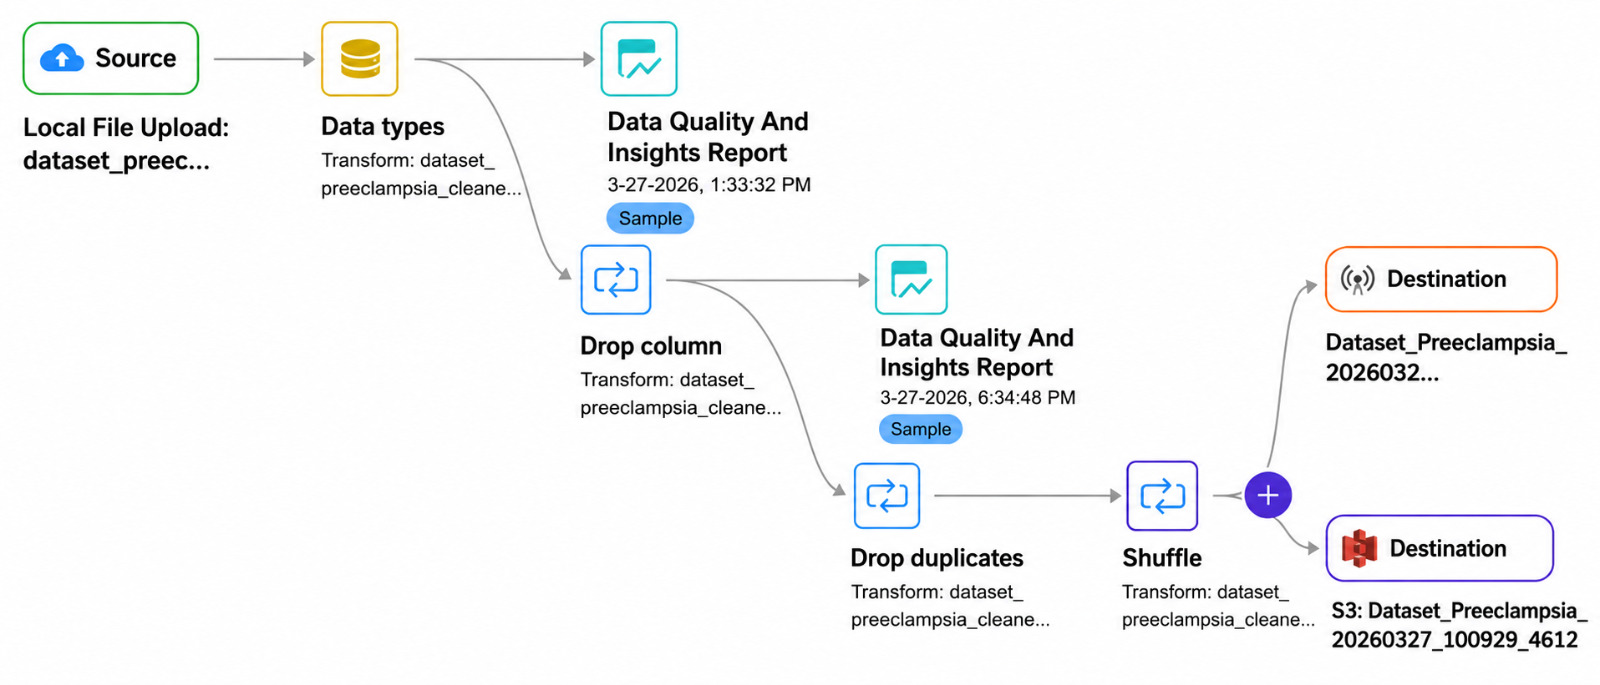
\includegraphics[width=1.2\textwidth]{figures/AWS-Wrangler-MP.jpeg}    %  figures/WranglerPreeclampsia.drawio2.png
  \end{adjustwidth}
  \caption{\label{fig:aws-wrangler}Data Wrangler is used to assess the
    quality of data before training the Machine Learning model. Low
    predictive power columns and duplicated records were
    removed. Resulting data is shuffled to prevent data leakage}
\end{figure}

\vspace{-9pt}
% R1.1 BEGIN: New table — dataset characteristics across preprocessing stages.
% Added per Reviewer 1 comment (Materials and Methods): "Add table with dataset
% characteristics: number of patients, class distribution, missing data rate
% and handling."  All figures verified against code/verify_patient_split.py.

\begin{table}[H]
  \small
  \centering
  \caption{Summary of dataset characteristics for the
    \ac{HGOIA} preeclampsia classification dataset. Each record corresponds
    to a prenatal clinical visit; a single patient may contribute multiple
    records across\mbox{ visits.}\label{tab:dataset-characteristics}}
  \begin{adjustwidth}{-\extralength}{0cm}
  \begin{tabularx}{\linewidth}{Ll}
    \toprule
    \textbf{Characteristic} & \textbf{Value} \\
    \midrule
    Data collection period & 2022--2025 \\
    Total records after ICD-10 filter and overlap removal & {4245} \\
    Unique patients (source dataset) & {2344} \\
    Average records per patient & 1.81 (range: 1--13) \\
    Duplicate/low-signal records removed (Canvas) & 80 (1.88\%) \\
    \midrule
    {Final {ML} dataset---total records} %MDPI: Please add an
                                %explanation for the use of bold in
                                %the table footer. If the bold is
                                %unnecessary, please remove it. The
                                %following highlights are the same. <<AUTHORS:agree>>
 & {4165} \\
    No preeclampsia---class~0 & {3494} (83.89\%) \\
    Preeclampsia---class~1 & 671 (16.11\%) \\
    Class imbalance ratio (class~0:class~1) & 5.2:1 \\
    \midrule
    Initial column-level missingness (pre-cleaning) & 12.9\% \\
    Missing data handling & Columns with high missingness removed; no imputation applied \\
    Missing values in final dataset & 0 \\
    \midrule
    Predictor features & 4 ({age, weight, {BMI}, gestational
                         weeks}) %MDPI: Please add an explanation for
                                %the use of italic in the table
                                %footer. If the italic is unnecessary,
                                %please remove it. The following
                                %highlights are the same. <<AUTHORS: agree>>
 \\
    Train/validation split (\ac{C-AutoML}) & 80\%/20\%, record-level, stratified by class \\
    \bottomrule
  \end{tabularx}
  \end{adjustwidth}
\end{table}
% R1.1 END

\subsection{Statistical Characteristics of Collected Data}
\label{sec:stat-char-data}

{Table}~\ref{tab:desc_stats} presents
statistical characteristics of demographic variables in the dataset,
whereas Table~\ref{tab:variable_distribution} shows the distribution
of those variables organized in quartiles \ac{w.r.t.} the
prevalence of \ac{PE} in pregnancies at \ac{HGOIA}. {We analyzed the prevalence of} \ac{PE} among the population
of pregnancies at the dataset provided by \ac{HGOIA}. Some
of the important insights are that \ac{PE} prevalence rises strongly
with age, reaching 85.13\% in the 36--49 year group
({Table} %MDPI: Please cite  the  first citation of each table
            %appears in numerical order. Now Table 5 cited before
            %Table 4, please check and revise <<AUTHORS: we changed
            %the order of the sentences to account for the order of
            %appearance of the tables>>
 \ref{tab:variable_distribution}). Women diagnosed
with \ac{PE} have a mean \ac{BMI} of 33. Normal pregnancies
have a mean \ac{BMI} of 25.71. These results are summarized in
Figure~\ref{fig:statistics}. 

% The record-level \ac{PE} prevalence in the final \ac{ML} dataset
% is 16.11\% (671 of 4,165 records); at the patient level, 588 of the 2,344 unique
% patients (25.1\%) received a \ac{PE} diagnosis. Both figures substantially exceed
% the global pooled estimate of approximately 4.43\%~\cite{vera2025preeclampsia},
% reflecting that \ac{HGOIA} is a public hospital specialised in gynaecology and
% obstetrics in Quito and that Ecuador's public health system directs high-risk
% pregnancies toward specialised facilities under a tiered zonification model
% coordinated by the \ac{MSP}. This elevated base rate directly affects the reported
% performance metrics: precision and \ac{F1} are calibrated to the cohort prevalence
% and would be expected to decrease in lower-prevalence settings.
% Table~\ref{tab:desc_stats} and Table~\ref{tab:variable_distribution} provide
% inter-group comparisons of all model input variables between \ac{PE}-positive
% and \ac{PE}-negative groups, with statistical significance tests.
\textls[-25]{The record-level prevalence of \ac{PE} in the final
  dataset is 16.11\% (671 of 4165 records), exceeding the global
  pooled estimate of 4.43\%~\cite{vera2025preeclampsia}. This
  reflects two factors: the dataset was constructed from a
  case-enriched selection of \ac{ICD-10} codes
  (Section~\ref{sec:data-preprocessing}) rather than the full
  obstetric population, and \ac{HGOIA} is a specialized referral
  centre that receives high-risk pregnancies directed by the
  \ac{MSP}. As a result, the reported precision and \ac{F1} are
  calibrated to this cohort prevalence and would decrease in
  lower-prevalence settings. \mbox{Tables~\ref{tab:desc_stats} and
  \ref{tab:variable_distribution}} provide inter-group
  comparisons of all model input variables between \ac{PE}-positive
  and \ac{PE}-negative groups; all four predictors show highly
  significant differences (Mann--Whitney $U$ and Pearson
  $\chi^2$, $p < 0.001$ for all variables), confirming their
  discriminative value within this cohort.}


\begin{table}[H]
  \small
%  \centering
  \caption{Descriptive statistics of demographic variables by
  preeclampsia diagnosis in pregnant women at \ac{HGOIA}
  from years 2022 to 2025. Statistics are computed on the
  pre-deduplication cohort (4245 records: 3571 normal, 674 
  preeclampsia); the final ML dataset after Canvas processing
  contains 4165 records (see Table~\ref{tab:dataset-characteristics}).}
\begin{tabularx}{\textwidth}{lp{2.cm}XXXXr}
% R1.2 BEGIN: Sample sizes and statistics are from the pre-deduplication cohort
% (dataset_preeclampsia_cleaned.csv, 4245 records: 3571 normal / 674 PE).
% This is what 02-explore-cleaned-data.ipynb computes. Caption updated to
% clarify the cohort; tab:dataset-characteristics shows the final ML counts.
% R2: p-value column added (Mann-Whitney U, two-sided; 05-statistical-tests-p-values.ipynb)
\toprule
\textbf{Variable} & \textbf{Preeclampsia} & \textbf{Sample Size} & \textbf{Mean} & \textbf{Median} & \textbf{Std.\ Dev.} & \textbf{\boldmath{$p$}-Value} \textbf{\textsuperscript{a}} \\
\midrule
AGE (YEARS) & No & 3571 & 18.71 & 18.00 & 4.13 & \multirow{2}{*}{$<$0.001} \\
          & Yes & 674  & 29.72 & 30.00 & 7.17 &  \\
\midrule
BMI       & No & 3571 & 25.71 & 25.19 & 4.39 & \multirow{2}{*}{$<$0.001} \\
          & Yes & 674  & 33.00 & 32.63 & 6.02 &  \\
\midrule
GESTATIONAL  & No & 3571 & 27.55 & 27.70 & 7.76 & \multirow{2}{*}{$<$0.001} \\
WEEKS                   & Yes & 674  & 33.80 & 35.40 & 4.42 &  \\
\midrule
WEIGHT    & No & 3571 & 61.20 & 59.50 & 11.67 & \multirow{2}{*}{$<$0.001} \\
          & Yes & 674  & 80.51 & 78.75 & 16.17 &  \\
\bottomrule
\end{tabularx}
\noindent\footnotesize{\textsuperscript{a} Mann--Whitney $U$ test, two-sided; compares each variable between the preeclampsia and normal groups.}
\label{tab:desc_stats}
\end{table}
% R1.2 END


\begin{figure}[H]
  \begin{adjustwidth}{-\extralength}{0cm}
    \centering
    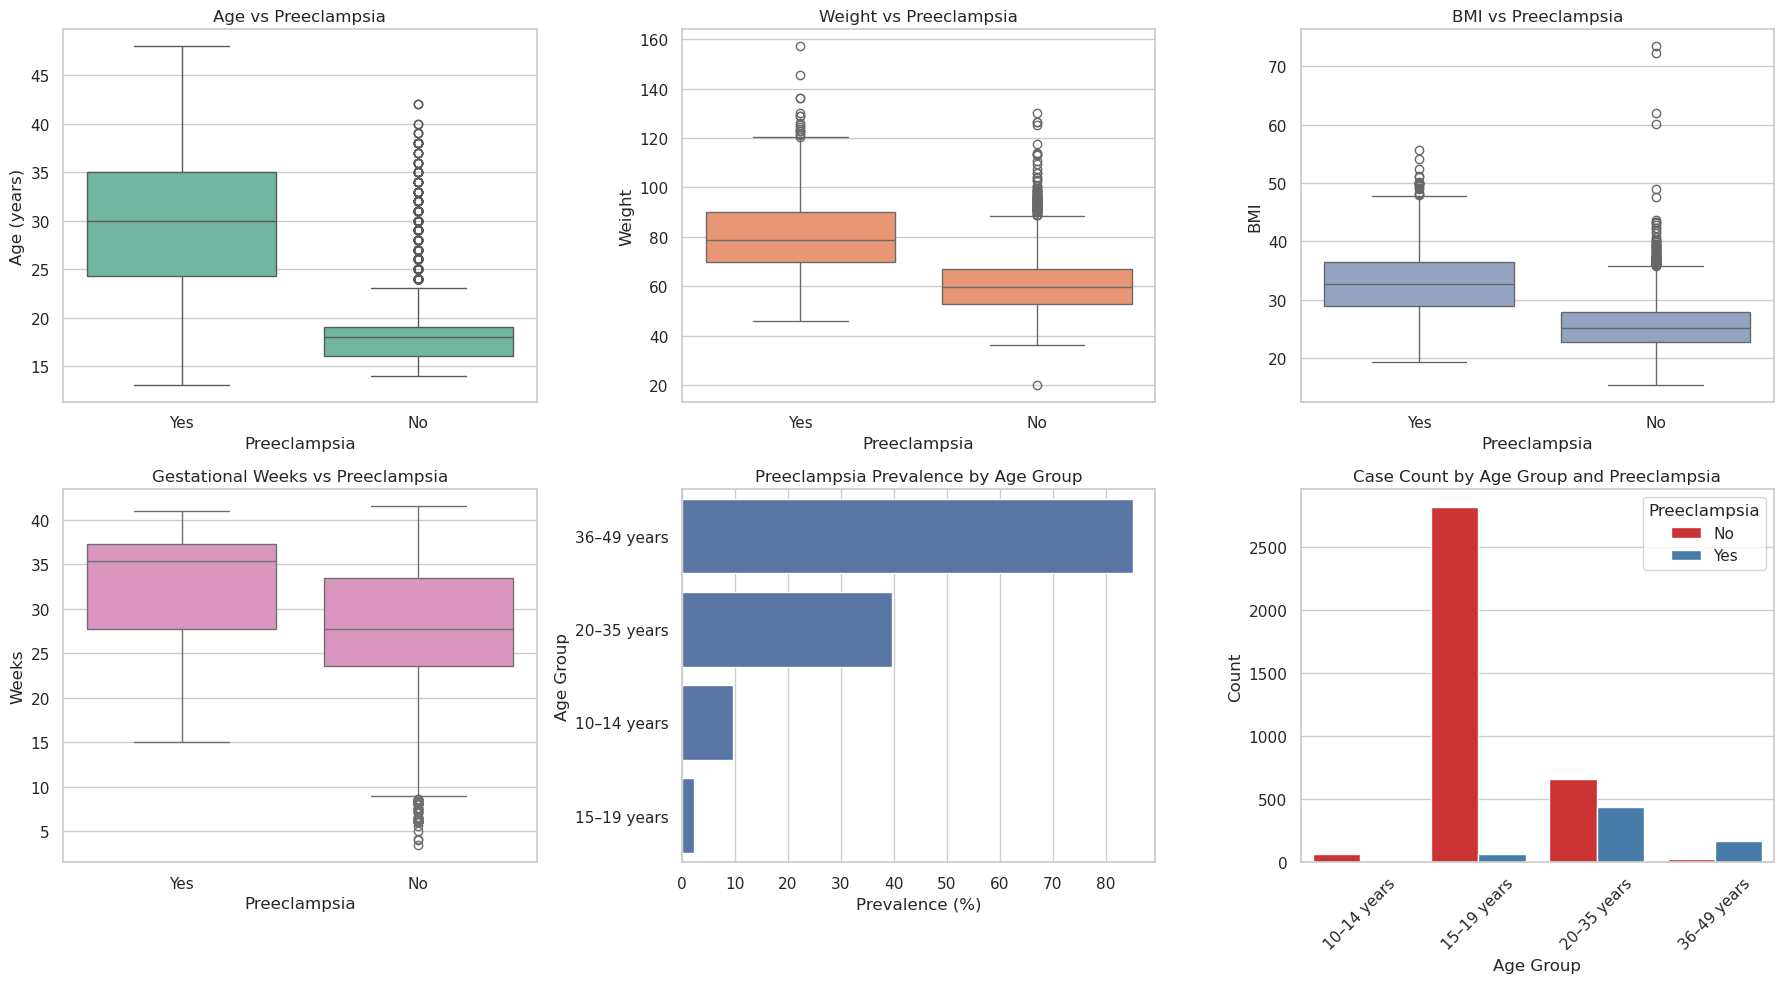
\includegraphics[width=\textwidth]{figures/dataset-statistics-HIA.png}
  \end{adjustwidth}
  \caption{\label{fig:statistics}{Statistical} %MDPI: Please
                                %confirm whether an explanation of the
                                %circles/colors needs to be added to
                                %the figure caption. <<AUTHOR: We
                                %think reader must be familiar with
                                %basic statistics. Unless a different
                                %criteria from you we would only add:
                                %"Circles denote outlier values beyond the interquartile range whiskers."
 analysis of prevalence of
    preeclampsia in the population of pregnant women at \ac{HGOIA}. Preeclampsia is more frequent in women of 36 to 49 years
  old and with a mean BMI of 33. Analysis based on the pre-deduplication
  cohort (4245 records: 3571 normal, 674 preeclampsia; see also
  Table~\ref{tab:dataset-characteristics}).}
\end{figure}

\vspace{-9pt}

\begin{table}[H]
  \small
%\centering
\caption{Distribution of pregnancies and preeclampsia prevalence
  across demographic concentration quartiles in women at \ac{HGOIA}
  from years 2022 to 2025.}

\begin{adjustwidth}{-\extralength}{0cm}
%\centering %% If there is a figure in wide page, please release command \centering, for Table, ``\textwidth" should be ``\fulllength"
\begin{tabularx}{\fulllength}{LLLLLLl}
% R2: p-value column added (Pearson chi-squared; 05-statistical-tests-p-values.ipynb)
\toprule
\textbf{Variable} & \textbf{Bin (Range)} & \textbf{Total Pregnancies} & \textbf{Normal Pregnancies} & \textbf{Preeclampsia Pregnancies} & \textbf{Preeclampsia Prevalence (\%)} & \textbf{\boldmath{$p$}-Value} \textbf{\textsuperscript{b}} \\
\midrule
AGE         & (12.999, 17.0] & 1745 & 1704 & 41 & 2.35\% & \multirow{4}{*}{$<$0.001} \\
(YEARS)     & (17.0, 18.0]   & 690  & 670  & 20  & 2.90\% &  \\
            & (18.0, 22.0]   & 797  & 735  & 62  & 7.78\% &  \\
            & (22.0, 48.0]   & 1013 & 462  & 551 & 54.39\% &  \\
\midrule
AGE GROUP   & 10–14 years    & 73   & 66   & 7   & 9.59\% & \multirow{4}{*}{$<$0.001} \\
            & 15–19 years    & 2877 & 2813 & 64  & 2.22\% &  \\
            & 20–35 years    & 1100 & 663  & 437 & 39.73\% &  \\
            & 36–49 years    & 195  & 29   & 166 & 85.13\% &  \\
\midrule
BMI         & (15.329, 23.18] & 1063 & 1041 & 22  & 2.07\% & \multirow{4}{*}{$<$0.001} \\
            & (23.18, 25.93]  & 1064 & 1014 & 50  & 4.70\% &  \\
            & (25.93, 29.42]  & 1058 & 935  & 123 & 11.63\% &  \\
            & (29.42, 73.46]  & 1060 & 581  & 479 & 45.19\% &  \\
\midrule
GESTATIONAL & (3.399, 26.0]   & 1066 & 1055 & 11  & 1.03\% & \multirow{4}{*}{$<$0.001} \\
WEEKS       & (26.0, 27.696]  & 1229 & 1062 & 167 & 13.59\% &  \\
            & (27.696, 35.2]  & 904  & 760  & 144 & 15.93\% &  \\
            & (35.2, 41.5]    & 1046 & 694  & 352 & 33.65\% &  \\
\midrule
WEIGHT      & (19.799, 54.0]  & 1086 & 1065 & 21  & 1.93\% & \multirow{4}{*}{$<$0.001} \\
            & (54.0, 61.5]    & 1043 & 1002 & 41  & 3.93\% &  \\
            & (61.5, 71.5]    & 1064 & 937  & 127 & 11.94\% &  \\
            & (71.5, 157.2]   & 1052 & 567  & 485 & 46.10\% &  \\
\bottomrule
\end{tabularx}
\end{adjustwidth}
\noindent\footnotesize{\textsuperscript{b} Pearson chi-squared test of independence between variable bin and preeclampsia status.}
\label{tab:variable_distribution}
\end{table}

\subsection{Synthetic Data Generation}
\label{sec:synth-data-gener}

To complement the retrospective demographic dataset from \ac{HGOIA} and compensate for
limited availability of structured clinical variables, we generated a
synthetic dataset designed to simulate clinical data profiles for
pregnant patients with and without \ac{PE}. The generation process was
implemented in {Python}~(3.9.23) %MDPI: Please state which version
                                %of the software was
                                %used. <<AUTHORS:removed the > symbold
                                %and stated version, the idea was that
                                %our code would work starting on that
                                %version to others.>>
  using {NumPy}~(2.0.2) and
{pandas}~(2.3.1), with a fixed random seed for
reproducibility. %<<AUTHORS: we removed special font \texttt>>

The algorithm generates $n={2000}$ samples (default: $n=1000$) and first
assigns each sample to one of two latent groups: {Control}
(80\%) or {Risk} (20\%). %<<AUTHORS: Removed italic formatting from group names ``Control'' and ``Risk'' as per MDPI guidelines on unnecessary special fonts.>> For each group, feature values are
sampled from predefined distributions chosen to reflect expected
clinical behavior. The generated variables are maternal age
($\mathrm{Age}$), \ac{GA}  in weeks ($\mathrm{GA_{wk}}$),
systolic and diastolic blood pressure (\ac{SBP}, \ac{DBP}),
24 h proteinuria, oxygen {saturation} ($\text{SpO}_2$), %<<AUTHOR:
                                %used same notation as in equation for SpO2>>
platelet count ($\mathrm{Plt}$), creatinine ($\upmu$mol/L),
\ac{AST}, and a chest pain indicator.
Table~\ref{tab:distributions} presents the statistical
distributions ($\mathcal{N}, \text{Gamma}, \text{Bernoulli}$) used
for the generation of each variable. Negative values were avoided
by clipping.

After feature generation, a binary diagnostic label
($\mathrm{PE}$) is assigned using a simplified rule based on the
Ecuadorian \ac{MSP} clinical guideline for \ac{HDP}~\cite{msp_ecuador_hdp_2013},
where \ac{HTN} denotes hypertension and \ac{ULN} denotes the upper limit of
normal for laboratory values.
Let \(\mathrm{HTN}=(\mathrm{SBP}\geq 140)\lor(\mathrm{DBP}\geq 90)\),
\(\mathrm{Prot}=(\mathrm{Prot_{24h}}\geq 300\,\mathrm{mg})\),
\(\mathrm{TCP}=(\mathrm{Plt}<100\times10^{9}\,\mathrm{L}^{-1})\),
\(\mathrm{Renal}=(\mathrm{Cr}_{\mathrm{mg/dL}}>1.1)\), and
\(\mathrm{Hep}\) for hepatic involvement defined as
\(\mathrm{AST}\geq 2\times\mathrm{ULN}\) with
\(\mathrm{ULN}=40\,\mathrm{U/L}\). Then,
\begin{linenomath}
\begin{equation}
\mathrm{PE}_{\mathrm{MSP}}=1
\iff
(\mathrm{GA_{wk}}\geq 20)\land \mathrm{HTN}
\land (\mathrm{Prot}\lor \mathrm{TCP}\lor \mathrm{Renal}\lor \mathrm{Hep}).
\label{eq:preeclampsia-msp-rule}
\end{equation}
\end{linenomath}

In addition to the binary diagnostic label, a continuous prognostic
risk score was computed using the published fullPIERS
model~\cite{fullpiers_2011}. For each sample, the algorithm computes a
logit function of \ac{GA}, chest {pain}, $\text{SpO}_2$, %
                                                            % <<AUTHOR:
                                                            % written
                                                            % SpO2 as
                                                            % in
                                                            % equation>>
$\mathrm{Plt}$, \ac{AST}, $\mathrm{Cr}$, and their interaction terms,
and then transforms it into a probability according
to~\eqref{eq:logistic-regression} and~\eqref{eq:fullpiers-logit}.
The final synthetic dataset therefore contains both a rule-based
diagnostic outcome ($\mathrm{PE}_{\mathrm{MSP}}$, defined in
Equation~\eqref{eq:preeclampsia-msp-rule}) and a continuous prognostic
risk estimate ($\mathrm{PE}_{\mathrm{FullPIERS}}$ [\%]), enabling exploratory
modeling and explainability analyses under clinically informed
constraints.

Although the $\mathrm{PE}_{\mathrm{FullPIERS}}$ score was used to
obtain an exploratory binary label with a threshold of $10\%$, empirical
validation studies have reported optimal cut-offs between 2 and 6\%
in different populations~\cite{long2025fullpiers,teichmann2025fullpiers,elongi2025fullpiers}.
For the diagnostic task on the synthetic dataset, however, the primary
classification target for model training and evaluation is the rule-based
label $\mathrm{PE}_{\mathrm{MSP}}$ defined in~\eqref{eq:preeclampsia-msp-rule},
which does not depend {on} $\text{SpO}_2$ % <<AUTHOR: uniform SpO>> or chest pain. Both variables are
nonetheless retained in the synthetic dataset because they are validated
independent predictors of adverse maternal outcomes in women with
established preeclampsia~\cite{millman2011spo2,elongi2025fullpiers}.

% The FullPIERS prognostic score was converted to a binary
%   label using a risk threshold of 10\% rather than the logistic
%   default of 50\%. In clinical screening and triage contexts the
%   adverse-outcome event is relatively uncommon. Consequently, few
%   patients reach a 50\% predicted probability on the FullPIERS scale,
%   which would result in very low sensitivity if the default threshold
%   were applied~\cite{fullpiers_2011}. A 10\% threshold captures
%   substantially more true high-risk pregnancies while accepting a
%   higher false-positive rate, consistent with the screening objective
%   of this component of the study. Empirical validation studies have
%   reported optimal thresholds ranging from approximately 2\% to 6\% in
%   different
%   populations~\cite{long2025fullpiers,teichmann2025fullpiers,elongi2025fullpiers},
%   further supporting the use of a sub-10\% cut-off for screening
%   purposes.  The primary classification target used for model training
%   and evaluation is the rule-based label $\mathrm{Preeclampsia\_MSP}$
%   (Equation~\eqref{eq:preeclampsia-msp-rule}); the FullPIERS-derived
%   binary label serves as a secondary prognostic reference for
%   exploratory analyses. The random seed was fixed at $\mathtt{42}$ to
%   ensure full reproducibility of the generation procedure.

% The features in this synthetic dataset are algorithmically
% generated from the parametric distributions specified in
% Table~\ref{tab:distributions} and were not measured in clinical
% practice; they do not form part of the \ac{HGOIA} retrospective records,
% which contain only demographic variables (age, weight, \ac{BMI}, and
% gestational age in weeks). The inclusion of SpO$_2$ and chest pain
% reflects their standing as validated independent predictors of adverse
% maternal outcomes in preeclampsia: SpO$_2$ values at or below 93\%
% carry an 18-fold increase in risk of severe complications within 48\,h
% of hospital admission~\cite{millman2011spo2}, a finding confirmed in
% recent independent cohorts~\cite{elongi2025fullpiers}, and both
% variables are explicit components of the FullPIERS prognostic equation
% (Equation~\eqref{eq:fullpiers-logit}; \cite{fullpiers_2011}).


\begin{table}[H]
  \small
%  \centering
  \caption{Statistical distributions for synthetic data generation.\label{tab:distributions}}
  % \begin{adjustwidth}{-\extralength}{0cm}
\begin{tabularx}{\textwidth}{CCCC}%llll
\toprule
\textbf{Feature} & \textbf{Control Group} & \textbf{Risk Group} & \textbf{Units} \\
\midrule
Age & $\mathcal{N}(27, 4)$ & $\mathcal{N}(33, 6)$ & years \\
Gestational age & $\mathcal{U}(34, 40)$ & $\mathcal{U}(26, 37)$ & weeks \\
Systolic BP & $\mathcal{N}(115, 8)$ & $\mathcal{N}(155, 12)$ & mmHg \\
Diastolic BP & $\mathcal{N}(75, 5)$ & $\mathcal{N}(102, 10)$ & mmHg \\
Proteinuria & $\text{Gamma}(2, 40)$ & $\mathcal{N}(1500, 700)$ & mg/24 h \\
$\text{SpO}_2$ & $\mathcal{N}(98, 1)$ & $\mathcal{N}(93, 3)$ & \% \\
Platelets & $\mathcal{N}(240, 40)$ & $\mathcal{N}(110, 55)$ & $10^9$/L \\
Creatinine & $\mathcal{N}(60, 10)$ & $\mathcal{N}(110, 40)$ & $\mu$mol/L \\
AST & $\mathcal{N}(25, 6)$ & $\mathcal{N}(90, 50)$ & U/L \\
Chest pain & $\text{Bernoulli}(0.03)$ & $\text{Bernoulli}(0.35)$ & binary \\
\bottomrule
\end{tabularx}
\noindent\footnotesize{Notes:} %<<AUTHORS: Removed italic from table footnote label as per MDPI guidelines on unnecessary special fonts.>>
$\mathcal{N}(\mu,\,\sigma)$: Normal distribution with mean $\mu$ and standard
deviation $\sigma$;
$\mathcal{U}(a,\,b)$: Uniform distribution over the interval $[a,\,b]$;
$\mathrm{Gamma}(k,\,\theta)$: Gamma distribution with shape parameter $k$ and
scale parameter $\theta$;
$\mathrm{Bernoulli}(p)$: Bernoulli variable with success probability $p$ (binary
outcome: 0 = absent, 1 = present).
% \end{adjustwidth}
\end{table}

\subsection{Machine Learning Models and Training}
\label{sec:mach-learn-models}
This research aims to diagnose \ac{PE} with the provided data
from \ac{HGOIA}. In Section~\ref{sec:materials-methods}, we
defined the \ac{PE} diagnostic problem as a binary
classification. Consequently, this study used two complementary
training tracks: (i) a cloud-managed workflow in Amazon SageMaker Canvas
for rapid no-code benchmarking, and (ii) \ac{C-AutoML} for controlled
experimentation and methodological traceability (see
Appendix~\ref{app:c-automl}). 

\subsubsection{Model Families}
\label{sec:model-families}

We evaluated six supervised model families commonly used in binary
classification, including gradient-boosted decision trees (XGBoost,
LightGBM, and CatBoost), \ac{RF}, \ac{MLP}, and regularized
\ac{LR}.

\begin{itemize}
\item {Logistic Regression (LR)}: A linear probabilistic
  baseline with high interpretability and robust behavior in
  tabular clinical settings~\cite{cox1958logistic}. %<<AUTHORS: removed bold>>%
\item {Random Forest (RF):} A bagging-based tree ensemble that
  captures non-linear interactions and is robust to noisy
  predictors~\cite{breiman2001randomforest}.%<<AUTHORS: removed bold>>%
\item {Multi-Layer Perceptron (MLP):} A feed-forward
  model able to represent higher-order non-linear
  relationships~\cite{rumelhart1986backprop}.%<<AUTHORS: removed bold>>%
\item {XGBoost:} Gradient-boosted decision trees with
  regularization and optimized implementation for strong predictive
  performance on structured data~\cite{chen2016xgboost}.%<<AUTHORS: removed bold>>%
\item {LightGBM:} A histogram-based gradient boosting framework
  designed for computational efficiency and scalability on large
  tabular datasets~\cite{ke2017lightgbm}.%<<AUTHORS: removed bold>>%
\item {CatBoost:} An ordered boosting method with native support
  for categorical variables and reduced prediction
  shift~\cite{prokhorenkova2018catboost}.%<<AUTHORS: removed bold>>%
\end{itemize}

\subsubsection{Training Process}
\label{sec:training-process}
Figure~\ref{fig:training-framework} illustrates the proposed
Machine Learning training framework used in this study, including the
parallel cloud-managed and script-based workflows.

% graph made by prism
\begin{figure}[H]
  \begin{adjustwidth}{-\extralength}{0cm}
    \centering
    \begin{tikzpicture}[node distance=6mm,box/.style={rectangle,
        rounded corners, draw=black, align=center, minimum
        width=4.8cm, minimum height=8mm,
        fill=gray!8},smallbox/.style={rectangle, rounded corners,
        draw=black, align=center, minimum width=4.5cm, minimum
        height=7mm, fill=gray!4},arrow/.style={-{Latex[length=2mm]},
        thick}]
      \node[box] (data) {Curated training dataset};
      \node[box, below left=12mm and 2mm of data] (cloud)
      {Cloud-managed workflow\\Amazon SageMaker Canvas};
      \node[box, below right=12mm and 2mm of data] (script) {Custom
        automated ML pipeline\\\texttt{autopilot\_train.py}};
      \node[smallbox, below=of cloud] (cloudprep) {Profiling, feature
        screening,\\model benchmarking};
      \node[smallbox, below=of script] (scriptprep) {Iterative
        stratified splits +\\random hyperparameter search};
      \node[smallbox, below=of cloudprep] (cloudmodels) {Cloud
        benchmarking and\\comparative diagnostics};
      \node[smallbox, below=of scriptprep] (scriptmodels) {Candidate
        models:\\LR, RF, ANN, XGBoost, LightGBM, CatBoost};
      \node[smallbox, below=of scriptmodels] (scriptpipe) {Model-aware
        pipelines:\\imputation, optional scaling, classifier};
      \node[box, below=30mm of $(cloudmodels)!0.5!(scriptmodels)$]
      (selection) {Model ranking and selection\\primary criterion:
        F1-score};
      \node[smallbox, below left=8mm and 2mm of selection] (perfout)
      {Performance outputs:\\metrics table, confusion matrix};
      \node[smallbox, below right=8mm and 2mm of selection] (shapout)
      {Explainability outputs:\\SHAP feature importance};
      \draw[arrow] (data) -- (cloud);
      \draw[arrow] (data) -- (script);
      \draw[arrow] (cloud) -- (cloudprep);
      \draw[arrow] (script) -- (scriptprep);
      \draw[arrow] (cloudprep) -- (cloudmodels);
      \draw[arrow] (scriptprep) -- (scriptmodels);
      \draw[arrow] (scriptmodels) -- (scriptpipe);
      \draw[arrow] (cloudmodels) -- (selection);
      \draw[arrow] (scriptpipe) -- (selection);
      \draw[arrow] (selection) -- (perfout);
      \draw[arrow] (selection) -- (shapout);
    \end{tikzpicture}%
        
  \end{adjustwidth}
  \caption{Proposed Machine Learning training framework combining
cloud-managed (SageMaker Canvas) and a custom automated ML pipeline
for model development, selection, performance evaluation, and
SHAP-based explainability.\label{fig:training-framework}}
\end{figure}

\paragraph{{Cloud-Managed Training (Amazon SageMaker Canvas)}}  % <<AUTHORS: To address MDPI's request on unnecessary bold formatting, we replaced manual bold text with a paragraph-style heading for consistent section formatting.>>
Amazon SageMaker Canvas (Amazon Web Services, Inc., Seattle, WA, USA)
is a managed no-code Machine Learning service that supports data
ingestion, preprocessing, model training, and model
evaluation~\cite{aws_sagemaker_canvas_docs}.  Internally, Canvas
relies on AutoGluon~\cite{agtabular2020} to manage the complete
training pipeline automatically. For our binary classification task,
Canvas was configured to maximize \ac{F1} and evaluated ten bagged
base model variants (Layer~1): LightGBM, LightGBM Extra Trees,
XGBoost, CatBoost, Random Forest (Gini), Random Forest (Entropy),
Extra Trees (Gini), Extra Trees (Entropy), FastAI neural network, and
{PyTorch} %MDPI: Please state which version of the software was
               %used. <<AUTHORS the version may change as it depends
               %on what AWS has at the moment, here PyTorch is
               %specified as the type of neural network implemented in
               %AWS since it uses two different neural networks one
               %PyTorch based and the other FastAI, this part is
               %controlled by AWS>>
  neural network, each trained on $k$-fold bagged splits of the
  training data. The final predictor is a two-layer weighted ensemble
  (Layer~2) built using AutoGluon's greedy forward ensemble selection
  algorithm~\cite{caruana2004ensemble}: starting from an empty
  ensemble, models are added one at a time (with replacement) if each
  addition improves the validation \ac{F1}. The weight assigned to
  each model $k$ equals its selection count $n_k$ divided by the total
  ensemble size~$S$:
\begin{linenomath}
\begin{equation}
  \hat{p}_{\mathrm{ens}}(\mathbf{x}) = \sum_{k=1}^{K} w_k\,\hat{p}_k(\mathbf{x}),
  \quad w_k = \frac{n_k}{S},
  \label{eq:ensemble-prediction}
\end{equation}
\end{linenomath}
where $\hat{p}_k(\mathbf{x})$ is the bag-averaged predicted
  probability from base model $k$, and the final binary decision applies
  threshold $\tau$ from Equation~\eqref{eq:preeclampsia_decision}.  In our
workflow, Canvas was also used for quality profiling and feature
screening support, as described in
Section~\ref{sec:data-preprocessing}.

\paragraph{{Custom Automatic Machine Learning Workflow (C-AutoML)}} % <<AUTHORS: To address MDPI's request on unnecessary bold formatting, we replaced manual bold text with a paragraph-style heading for consistent section formatting.>>
We proposed an iterative training methodology where different stratified
80/20 train/validation splits are tested on every model candidate
across $N = 10$ outer iterations, yielding 60 total trials
(10 iterations $\times$ 6 model families). The training core executes
an inner loop that iterates through six algorithm families: \ac{LR},
\ac{RF}, \ac{MLP}, XGBoost, LightGBM, and CatBoost.

For \ac{HPO}, C-AutoML adopts a {random search}
strategy~\cite{bergstra2012random}: %<<AUTHORS: Removed italic from ``random search''; it is a standard technical term that does not require special emphasis.>> at each trial, exactly one
hyperparameter configuration is drawn uniformly at random from a
predefined discrete candidate set using scikit-learn's
\texttt{ParameterSampler}~\cite{sklearn-api} (seed $= 42 + 100i + m$,
where $i$ is the outer-loop iteration and $m$ is the model-family
index). Random search is preferred over grid search because it
explores the hyperparameter space more efficiently at a fixed
computational budget~\cite{bergstra2012random}. The complete search
spaces are listed in Table~\ref{tab:hpo-search-spaces}.



% R1.5 BEGIN -------------------------------------------------------
\begin{table}[H]

\caption{C-AutoML hyperparameter search spaces.
    At each trial one configuration is drawn uniformly at random
    (\texttt{ParameterSampler}) from the Cartesian product of the listed
    candidate values.  Tree-based models omit StandardScaler;
    \ac{LR} and \ac{MLP} apply it.}
\label{tab:hpo-search-spaces}
\small
\begin{tabularx}{\linewidth}{LLL}
\toprule
\textbf{Model Family} & \textbf{Hyperparameter} & \textbf{Candidate Values} \\
\midrule
\multirow{3}{*}{Logistic Regression}
  & Regularization $C$          & \{0.01, 0.1, 1, 5, 10\} \\
  & Solver                      & \{\texttt{liblinear}, \texttt{lbfgs}\} \\
  & Class weight                & \{none, balanced\} \\
\midrule
\multirow{5}{*}{Random Forest}
  & No.\ of estimators          & \{200, 400, 600\} \\
  & Maximum depth               & \{none, 5, 10, 20\} \\
  & Min.\ samples per split     & \{2, 5, 10\} \\
  & Min.\ samples per leaf      & \{1, 2, 4\} \\
  & Class weight                & \{none, balanced, balanced\_subsample\} \\
\midrule
\multirow{3}{*}{MLP Neural Network}
  & Hidden-layer sizes          & \{(64), (128), (64,\,32), (128,\,64)\} \\
  & L2 penalty $\alpha$         & \{0.0001, 0.001, 0.01\} \\
  & Initial learning rate       & \{0.0005, 0.001, 0.005\} \\



\bottomrule
\end{tabularx}
\end{table}



\begin{table}[H]\ContinuedFloat   

\caption{\emph{Cont.}}
\label{tab:hpo-search-spaces}
\small
\begin{tabularx}{\linewidth}{LLL}
\toprule
\textbf{Model Family} & \textbf{Hyperparameter} & \textbf{Candidate Values} \\
\midrule


\multirow{5}{*}{XGBoost}
  & Maximum tree depth          & \{3, 4, 6, 8\} \\
  & Learning rate               & \{0.01, 0.05, 0.1, 0.2\} \\
  & Subsample ratio             & \{0.70, 0.85, 1.0\} \\
  & Column sample by tree       & \{0.70, 0.85, 1.0\} \\
  & L2 regularization $\lambda$ & \{1, 2, 5\} \\
\midrule
\multirow{5}{*}{LightGBM}
  & Maximum leaf count          & \{15, 31, 63\} \\
  & Learning rate               & \{0.01, 0.05, 0.1\} \\
  & Subsample ratio             & \{0.70, 0.85, 1.0\} \\
  & Column sample by tree       & \{0.70, 0.85, 1.0\} \\
  & L2 regularization $\lambda$ & \{0, 1, 5\} \\
\midrule
\multirow{4}{*}{CatBoost}
  & Tree depth                  & \{4, 6, 8\} \\
  & Learning rate               & \{0.01, 0.05, 0.1\} \\
  & Number of boosting rounds   & \{200, 400, 600\} \\
  & L2 leaf regularization      & \{1, 3, 5\} \\
\bottomrule
\end{tabularx}
\end{table}
% R1.5 END ---------------------------------------------------------

The proposed methodology fits full
\texttt{scikit-learn}~({1.6.1})~\cite{sklearn-api} %<<AUTHOR: we
                                %removed the > symbol to account for
                                %the exact version of the package
                                %used>>
pipelines with model-aware preprocessing (StandardScaler enabled for
\ac{LR} and \ac{MLP}; disabled for tree-based models) and handles
missing values using median imputation for numeric features and mode
imputation for categorical features. Model selection is obtained by
ranking all \mbox{60 trials} \ac{w.r.t.} \ac{F1} (primary metric,
selected to account for class imbalance), followed by \ac{AUC} and
overall \ac{ACC} as tie-breaking metrics. Upon identifying the optimal
pipeline, the system performs permutation-based feature importance
analysis ($n_{\mathrm{repeats}} = 10$, \ac{F1} scoring on the
validation partition) to enhance model interpretability.
Figure~\ref{fig:c-automl-flowchart} provides a flowchart overview of
the complete \ac{C-AutoML} pipeline.




\subsubsection{Evaluation Metrics}
\label{sec:evaluation-metrics}
Performance was evaluated with four complementary metrics: \ac{F1},
overall \ac{ACC}, \ac{AUC}, and confusion matrix analysis. In the
cloud-managed workflow (Amazon SageMaker Canvas), the target
optimization metric was \ac{F1}. For our proposed \ac{C-AutoML} pipeline,
\ac{F1} was also the primary model-selection criterion because it
balances precision and recall under class imbalance; ties in \ac{F1}
were resolved using \ac{AUC} and then overall \ac{ACC}:
\begin{linenomath}
\begin{equation}
\mathrm{F1}=2\times\frac{\mathrm{Precision}\times\mathrm{Recall}}{\mathrm{Precision}+\mathrm{Recall}}.
\label{eq:f1-score}
\end{equation}
\end{linenomath}

Overall \ac{ACC} was reported as the proportion of correctly
classified cases among all evaluated pregnancies:
\begin{linenomath}
\begin{equation}
\mathrm{Accuracy}=\frac{TP+TN}{TP+TN+FP+FN}.
\label{eq:accuracy}
\end{equation}
\end{linenomath}

Discrimination across thresholds was quantified with \ac{AUC}, where
higher values indicate better separation between \ac{PE} and
non-\ac{PE} classes~\cite{fawcett2006roc}.

Finally, the confusion matrix (\(TP, TN, FP, FN\)) was analyzed to
characterize the clinical error profile of each candidate model,
especially the trade-off between missed-risk cases and false
alerts~\cite{sokolova2009systematic,powers2011evaluation}.

% R1.4 BEGIN -------------------------------------------------------
\begin{figure}[H]

 %\includegraphics[width=\textwidth]{figure-1} 

\begin{adjustwidth}{-\extralength}{0cm}

\centering
\begin{tikzpicture}[
    node distance=0.5cm,
    every node/.style={font=\small},
    TermNode/.style={
        rectangle, rounded corners=5pt,
        draw=black!80, fill=gray!20, text centered,
        text width=9cm, minimum height=0.8cm, inner sep=4pt},
    ProcNode/.style={
        rectangle, draw=black!80, fill=white, text centered,
        text width=9cm, minimum height=0.8cm, inner sep=4pt},
    arr/.style={-Stealth, thick}
]
%% ---------- nodes ----------
\node (Ninput) [TermNode] {%
    \textbf{Input:} ML dataset (4165 records, 4 features) ---
    feature set pre-selected by SageMaker Canvas};

\node (Ninit) [ProcNode, below=of Ninput] {%
    Initialize 6 model families:
    \ac{LR}, \ac{RF}, \ac{MLP}, XGBoost, LightGBM, CatBoost};

%% outer loop top (extra gap for outer-loop label)
\node (Nsplit) [ProcNode, below=1.5cm of Ninit] {%
    Stratified 80/20 train\,/\,val split\\[-2pt]
    {\footnotesize (seed\;$= 42 + i$)}};

%% inner loop top (extra gap for inner-loop label)
\node (Nhpo) [ProcNode, below=1.2cm of Nsplit] {%
    Sample one \ac{HPO} configuration per model candidate\\[-2pt]
    {\footnotesize (ParameterSampler;\; seed $= 42 + 100i + m$)}};

\node (Npreproc) [ProcNode, below=of Nhpo] {%
    Build model-aware \texttt{sklearn} preprocessing pipeline\\[-2pt]
    {\footnotesize Numeric: median imputation
      [+\,StandardScaler if \ac{LR}/\ac{MLP}];\;
      Categorical: mode imputation + OHE}};

\node (Nfit) [ProcNode, below=of Npreproc] {%
    Fit \texttt{Pipeline}(preprocessor, model$_m$) on $X_{\!\mathrm{train}}$};

\node (Neval) [ProcNode, below=of Nfit] {%
    Evaluate on $X_{\!\mathrm{val}}$:\;
    F1, \ac{AUC}, \ac{ACC}, Precision, Recall};

\node (Nupdate) [ProcNode, below=of Neval] {%
    Update best trial record if F1 $>$ best$_{\mathrm{F1}}$};

%% post-loop
\node (Nselect) [ProcNode, below=1.2cm of Nupdate] {%
    Select best pipeline \quad (rank:\; F1 $\to$ \ac{AUC} $\to$ \ac{ACC})};

\node (Nperm) [ProcNode, below=of Nselect] {%
    Permutation importance analysis\\[-2pt]
    {\footnotesize ($n_{\mathrm{repeats}} = 10$,\;
      scoring: F1,\; applied on validation partition)}};

\node (Noutput) [TermNode, below=of Nperm] {%
    \textbf{Outputs:}\;
    serialized model\,$\cdot$\,
    metrics log\,$\cdot$\,
    confusion matrix\,$\cdot$\,
    feature importance ranking};

%% ---------- straight-down arrows ----------
\draw[arr] (Ninput)   -- (Ninit);
\draw[arr] (Ninit)    -- (Nsplit);
\draw[arr] (Nsplit)   -- (Nhpo);
\draw[arr] (Nhpo)     -- (Npreproc);
\draw[arr] (Npreproc) -- (Nfit);
\draw[arr] (Nfit)     -- (Neval);
\draw[arr] (Neval)    -- (Nupdate);
\draw[arr] (Nupdate)  --
    node[right, font=\scriptsize\itshape, fill=white, inner sep=1pt, pos=0.5]{all 60 trials complete}
    (Nselect);
\draw[arr] (Nselect)  -- (Nperm);
\draw[arr] (Nperm)    -- (Noutput);

%% ---------- loop-back arrows ----------
%% inner loop (right side): update -> right -> up -> hpo
\coordinate (ILmid) at ([xshift=1.8cm]Nupdate.east);
\draw[dashed, thick]
    (Nupdate.east) -- node[above, font=\scriptsize\itshape, fill=white, inner sep=1pt]{next model} (ILmid);
\draw[arr, dashed, thick] (ILmid) |- (Nhpo.east);

%% outer loop (left side): update -> left -> up -> split
\coordinate (OLmid) at ([xshift=-3.0cm]Nupdate.west);
\draw[dashed, thick]
    (Nupdate.west)
    -- node[above, font=\scriptsize\itshape, fill=white, inner sep=1pt]{next iteration}
    (OLmid);
\draw[arr, dashed, thick] (OLmid) |- (Nsplit.west);

%% ---------- background loop regions ----------
\begin{pgfonlayer}{background}
    %% outer box drawn first so inner orange sits visually on top
    \node[draw=blue!60!black, dashed, rounded corners=8pt,
          fill=blue!4, inner sep=16pt,
          fit=(Nsplit)(Nhpo)(Npreproc)(Nfit)(Neval)(Nupdate)
    ] (outer_box) {};
    %% inner box drawn second = on top of outer fill
    \node[draw=orange!80!black, dashed, rounded corners=5pt,
          fill=orange!8, inner sep=8pt,
          fit=(Nhpo)(Npreproc)(Nfit)(Neval)(Nupdate)
    ] (inner_box) {};
\end{pgfonlayer}

%% loop labels in the main layer so they render above all background fills
\node[font=\scriptsize\itshape, text=blue!70!black, fill=white,
      inner sep=1pt, anchor=south west]
     at (outer_box.north west)
     {outer loop ($N\!=\!10$ iterations,\;$i = 1\ldots10$,\;60 total trials)};
\node[font=\scriptsize\itshape, text=orange!80!black, fill=white,
      inner sep=1pt, anchor=south west]
     at (inner_box.north west)
     {inner loop (6 model families,\;$m = 1\ldots6$)};

\end{tikzpicture}
\end{adjustwidth}

\caption{{Flowchart} %MDPI:  1. Commas are only used for numbers
                        %with five or more digits. We removed them in
                        %four-digit numbers in the figure. Please
                        %confirm. 2. We move Figure 5 here to avoid
                        %blank, please check if it's ok <<AUTHORS: We
                        %agree on both matters>>
 of the \ac{C-AutoML} training
    pipeline. The outer loop runs $N = 10$ iterations
    ($i = 1\ldots10$), each drawing a fresh stratified 80/20
    train/validation split, for a total of 60 trials
    (10 iterations $\times$ 6 model families). Within each trial, one
    \acf{HPO} configuration is stochastically sampled from a
    predefined search space (ParameterSampler) and a model-aware
    \texttt{sklearn} pipeline is fitted on the training partition
    (median imputation; StandardScaler for \ac{LR}/\ac{MLP};
    OneHotEncoder for categorical variables). Candidates are ranked by
    F1-score (primary), \ac{AUC} (secondary), and \ac{ACC} (tertiary)
    across all 60 trials; the best pipeline is then selected and
    subjected to permutation importance analysis
    ($n_{\mathrm{repeats}} = 10$, F1 scoring) to rank feature
    contributions.}
\label{fig:c-automl-flowchart}
\end{figure}
% R1.4 END ---------------------------------------------------------



\section{Results}
\label{sec:results}
Our results will address the performance of the models (i) with the
provided data from the Isidro Ayora Gynecology and Obstetrics {Hospital}
(\ac{HGOIA}) % <<AUTHOR: added parenthesis to the acronym. The name of
             % the hospital is repeated to aid skimming
             % readers. However if MDPI thinks it is better to use the
             % acronym directly this should be modified>>
and (ii) with the synthetic clinical data that we produced. For the
former, we trained our models using Amazon SageMaker Canvas and our
proposed methodology \ac{C-AutoML}. For the latter, we only used
\ac{C-AutoML}.
\subsection{Performance of C-AutoML on \ac{HGOIA} Data}
\label{sec:performance-c-automl}

Our proposed methodology \ac{C-AutoML} achieved its best performance
on model LightGBM, with an $\mathrm{F1}=0.802$,
$\mathrm{Precision}=0.837$, $\mathrm{Recall}=0.768$, and
$\mathrm{AUC}=0.944$, on Trial\#23,
iteration\#4. Table~\ref{tab:cautoml-performance} presents the
complete performance of the different trials for each of the proposed
models. Each iteration uses a different train and validation split and
different
hyperparameters. Figure~\ref{fig:combined-model-analysis-isidro-ayora}
presents the normalized confusion
matrix (Figure~\ref{fig:combined-model-analysis-isidro-ayora}a), the feature
importance values (Figure~\ref{fig:combined-model-analysis-isidro-ayora}b), the
precision--recall curve
performance (Figure~\ref{fig:combined-model-analysis-isidro-ayora}c), and a comparison
\ac{w.r.t.} the \ac{F1} of the models trained
in Figure~\ref{fig:combined-model-analysis-isidro-ayora}d.

%Custom Automated Machine Learning Workflow Performance across 6
%different models. Each model is evaluated in different trials  with
%different train/validation splits and set of hyperparameters



\begin{figure}[H]
\begin{adjustwidth}{-\extralength}{0cm}
\centering
\subfloat[\centering \label{fig:confusion-matrix-bestmodel-cautoml}]{
  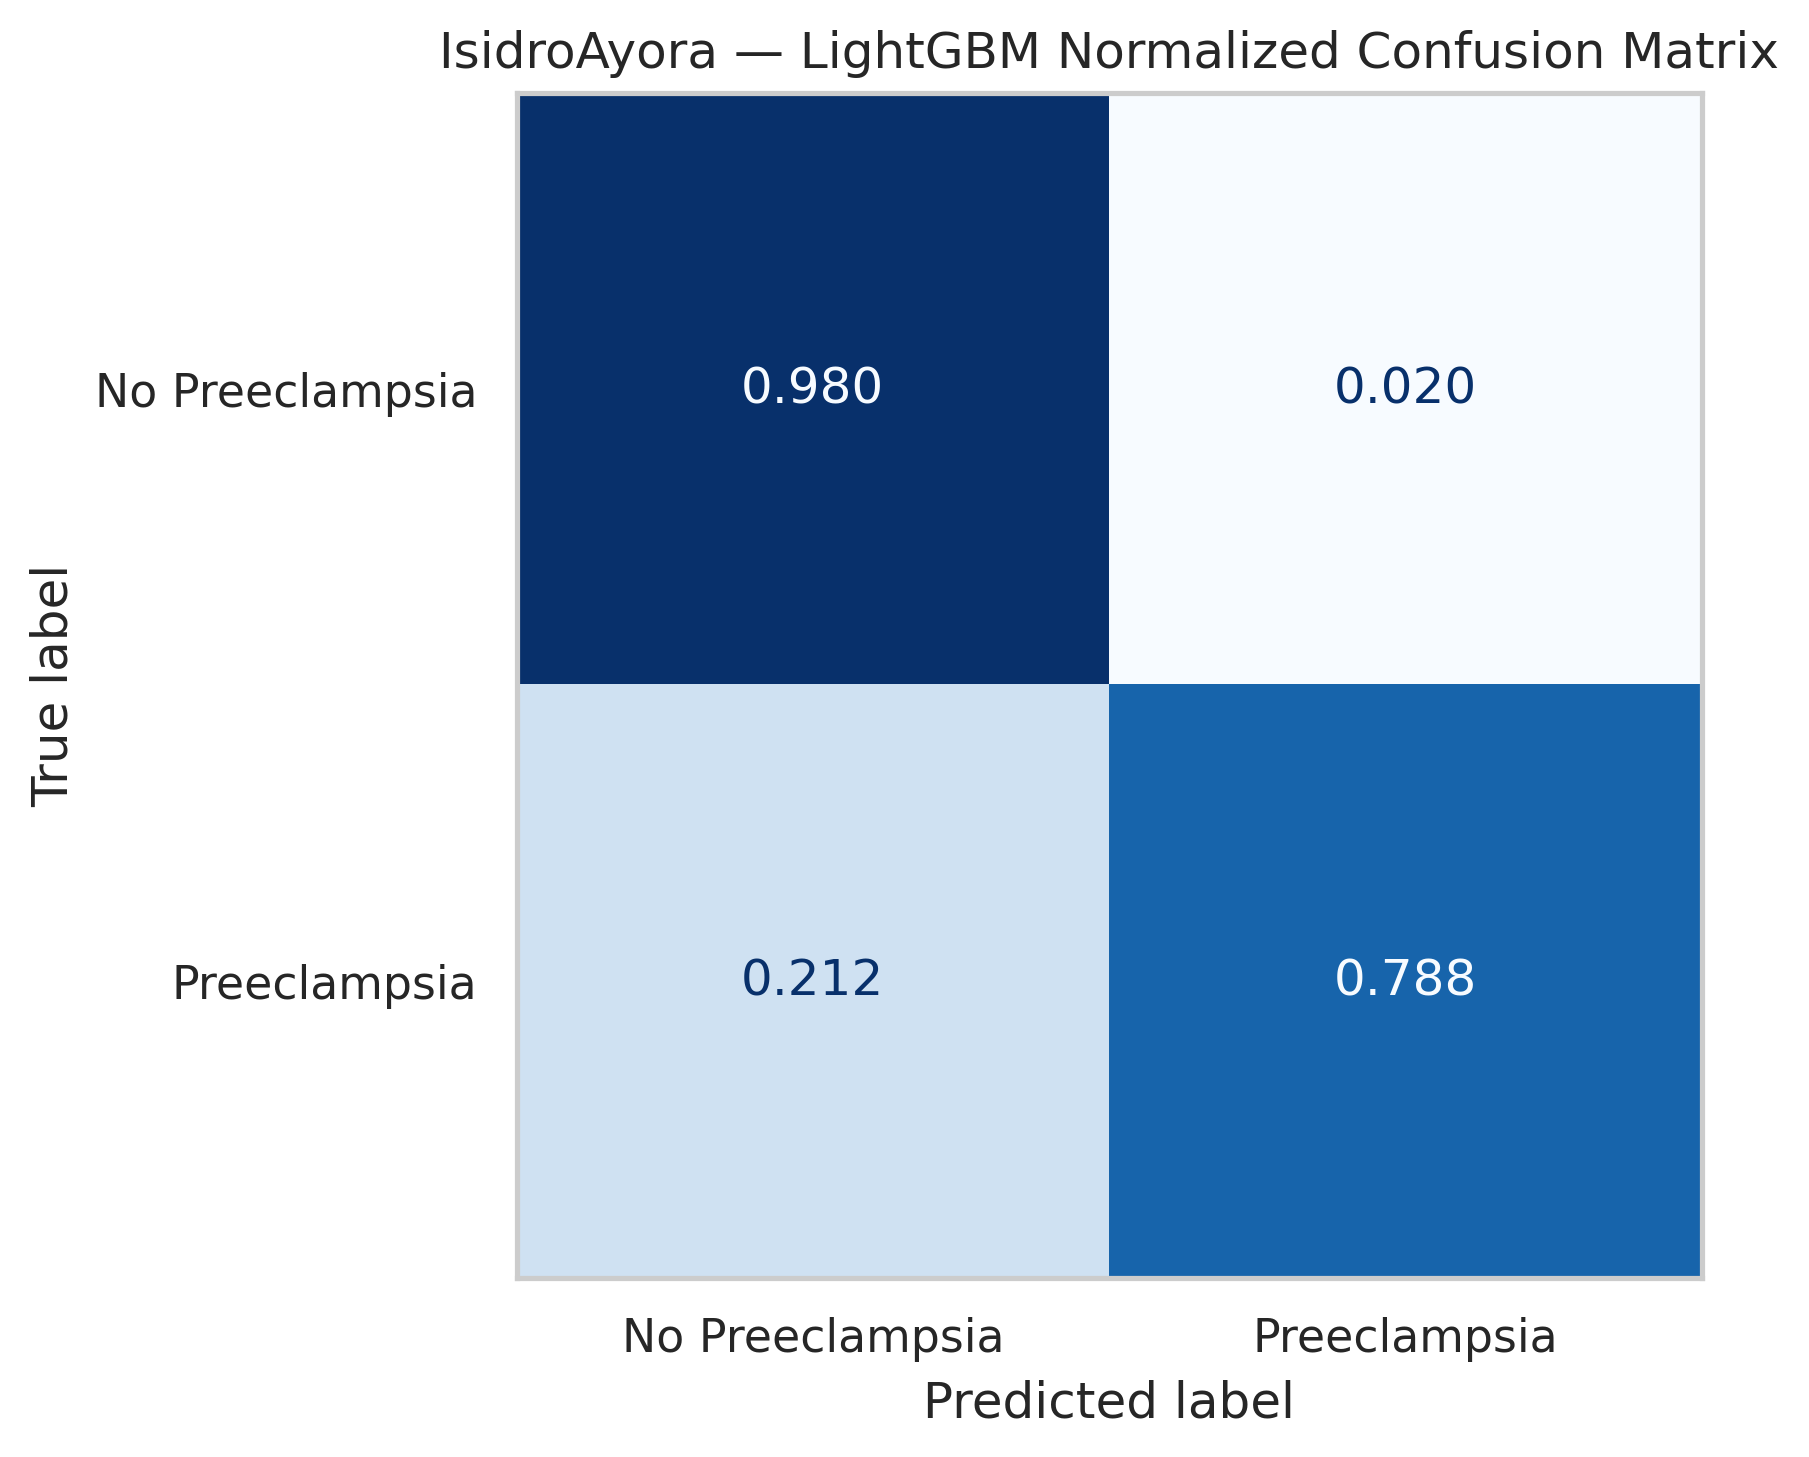
\includegraphics[width=0.48\fulllength]{figures/isidroayora_lightgbm_normalized_confusion_matrix.png}}
\subfloat[\centering\label{fig:feature-importance-lightgbm}]{
  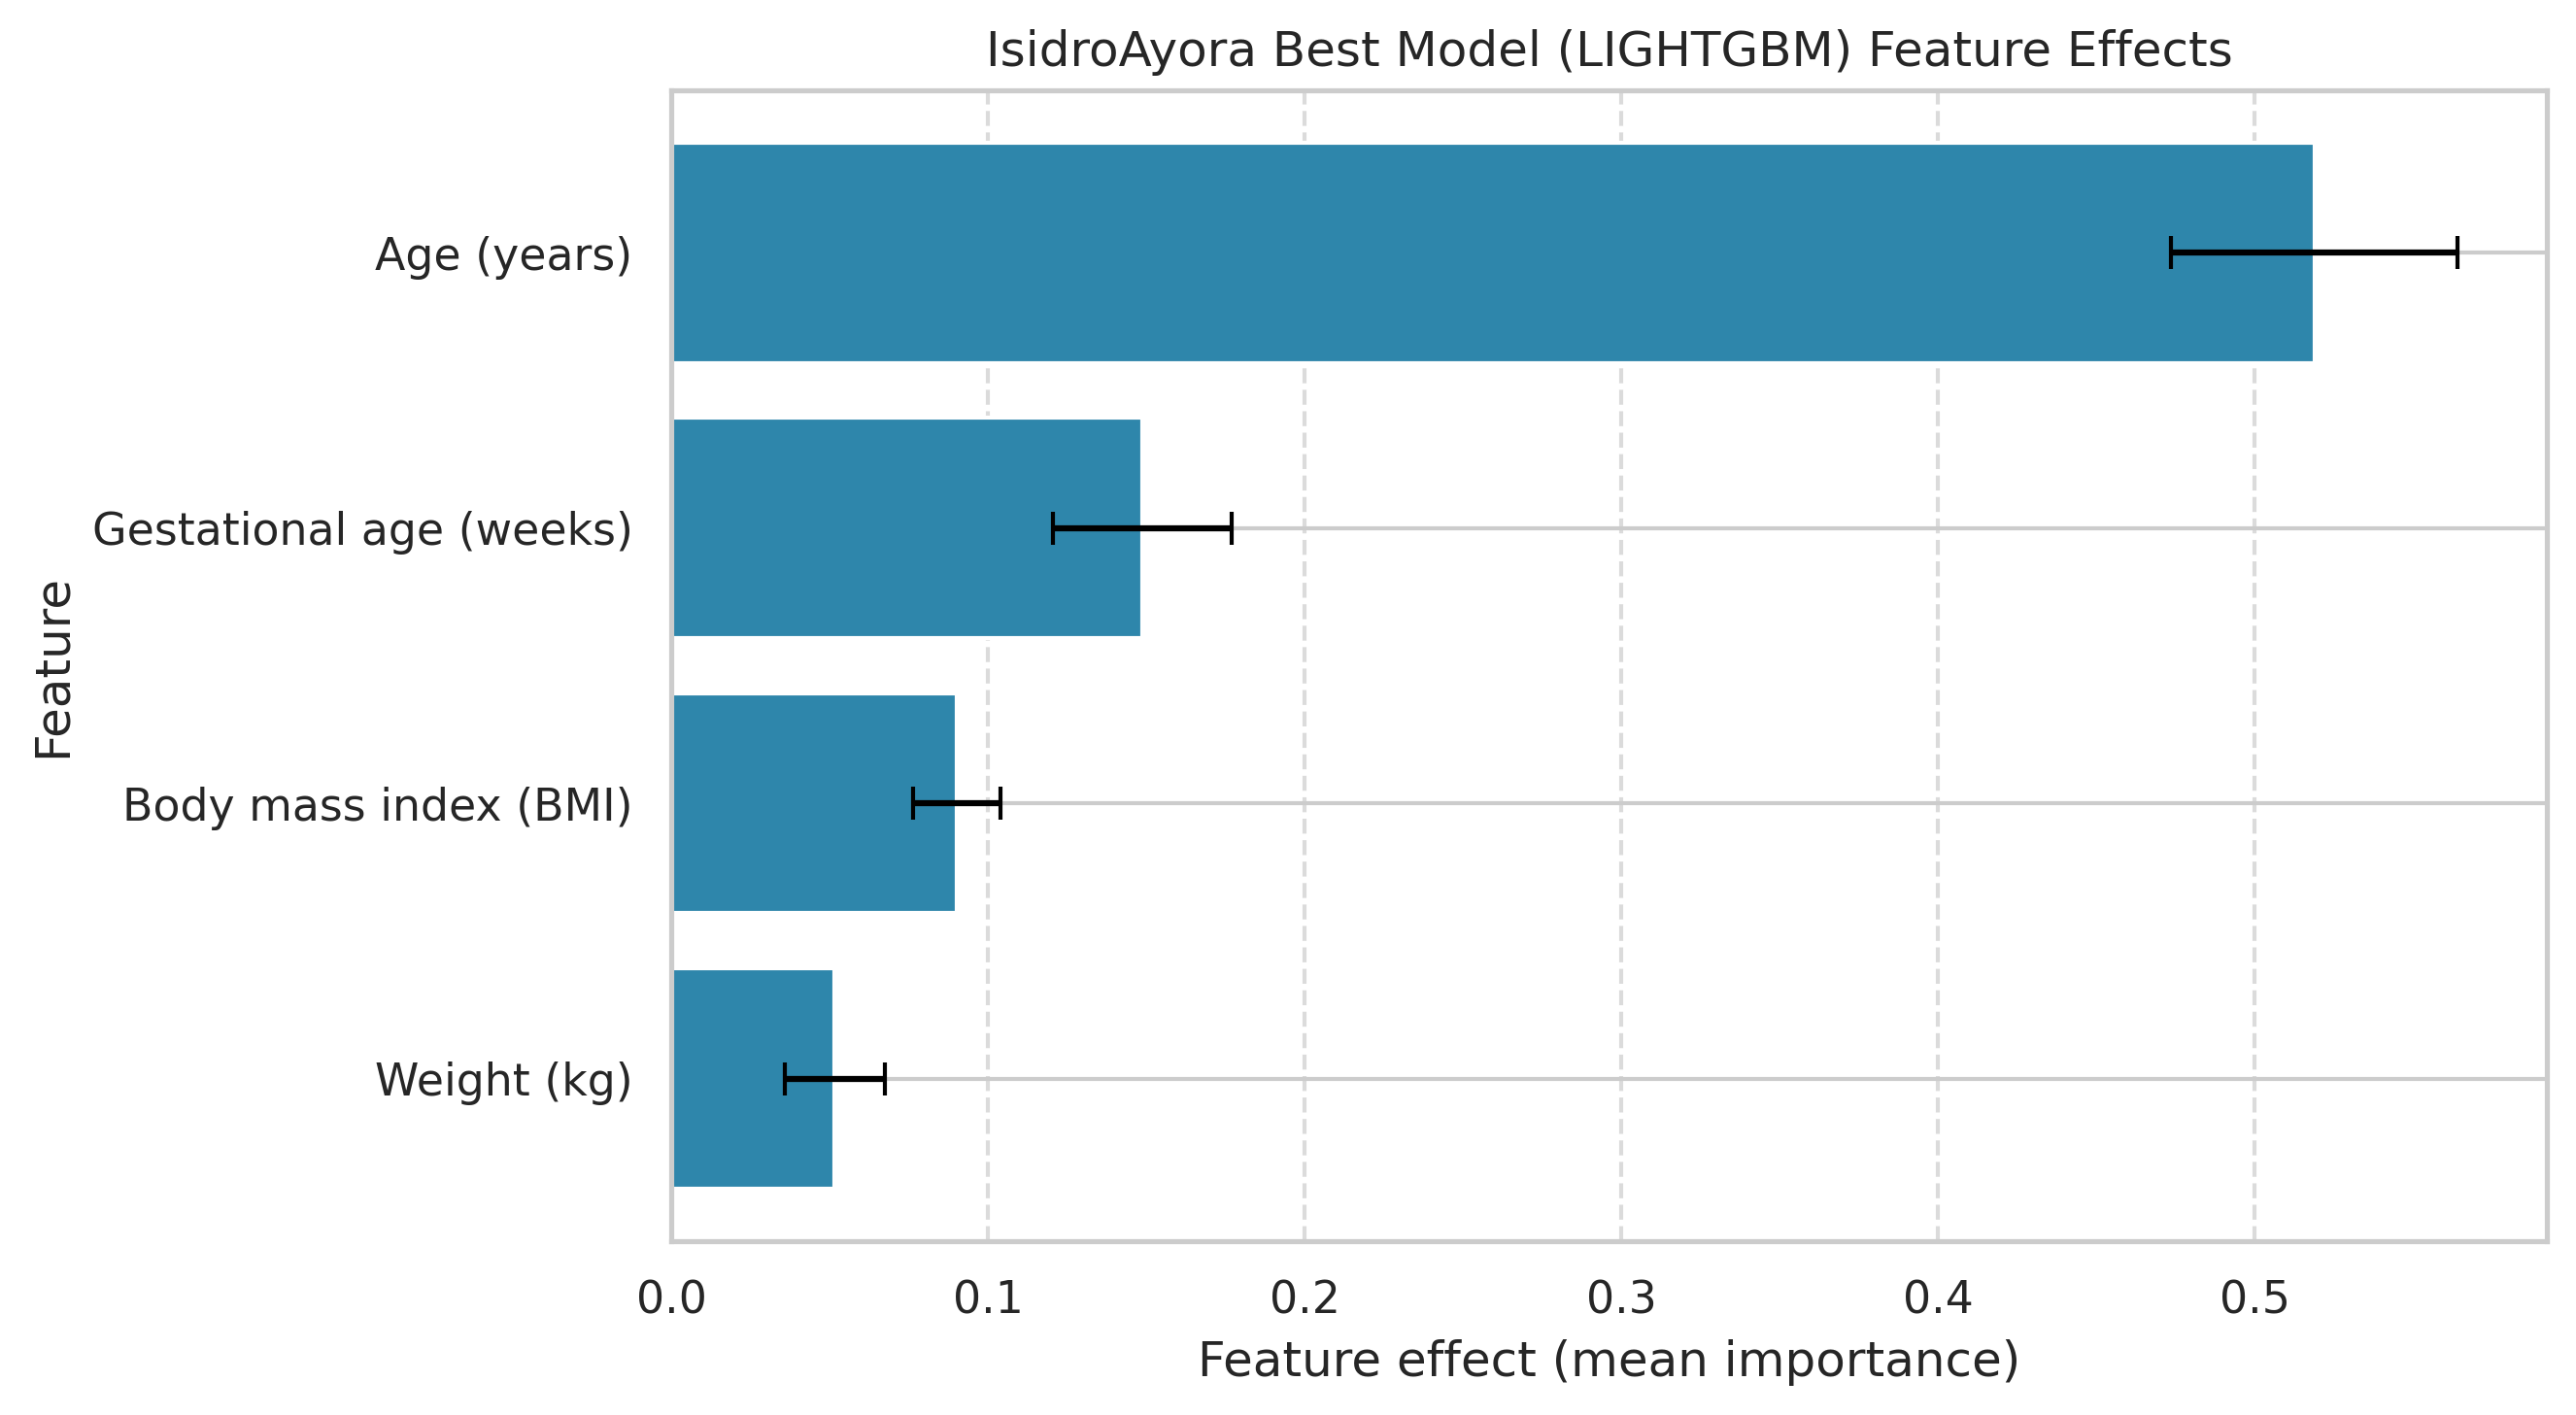
\includegraphics[width=0.48\fulllength]{figures/isidroayora_best_model_feature_effects_mean_std.png}}\\
\subfloat[\centering\label{fig:precision-recall-lightgbm}]{
  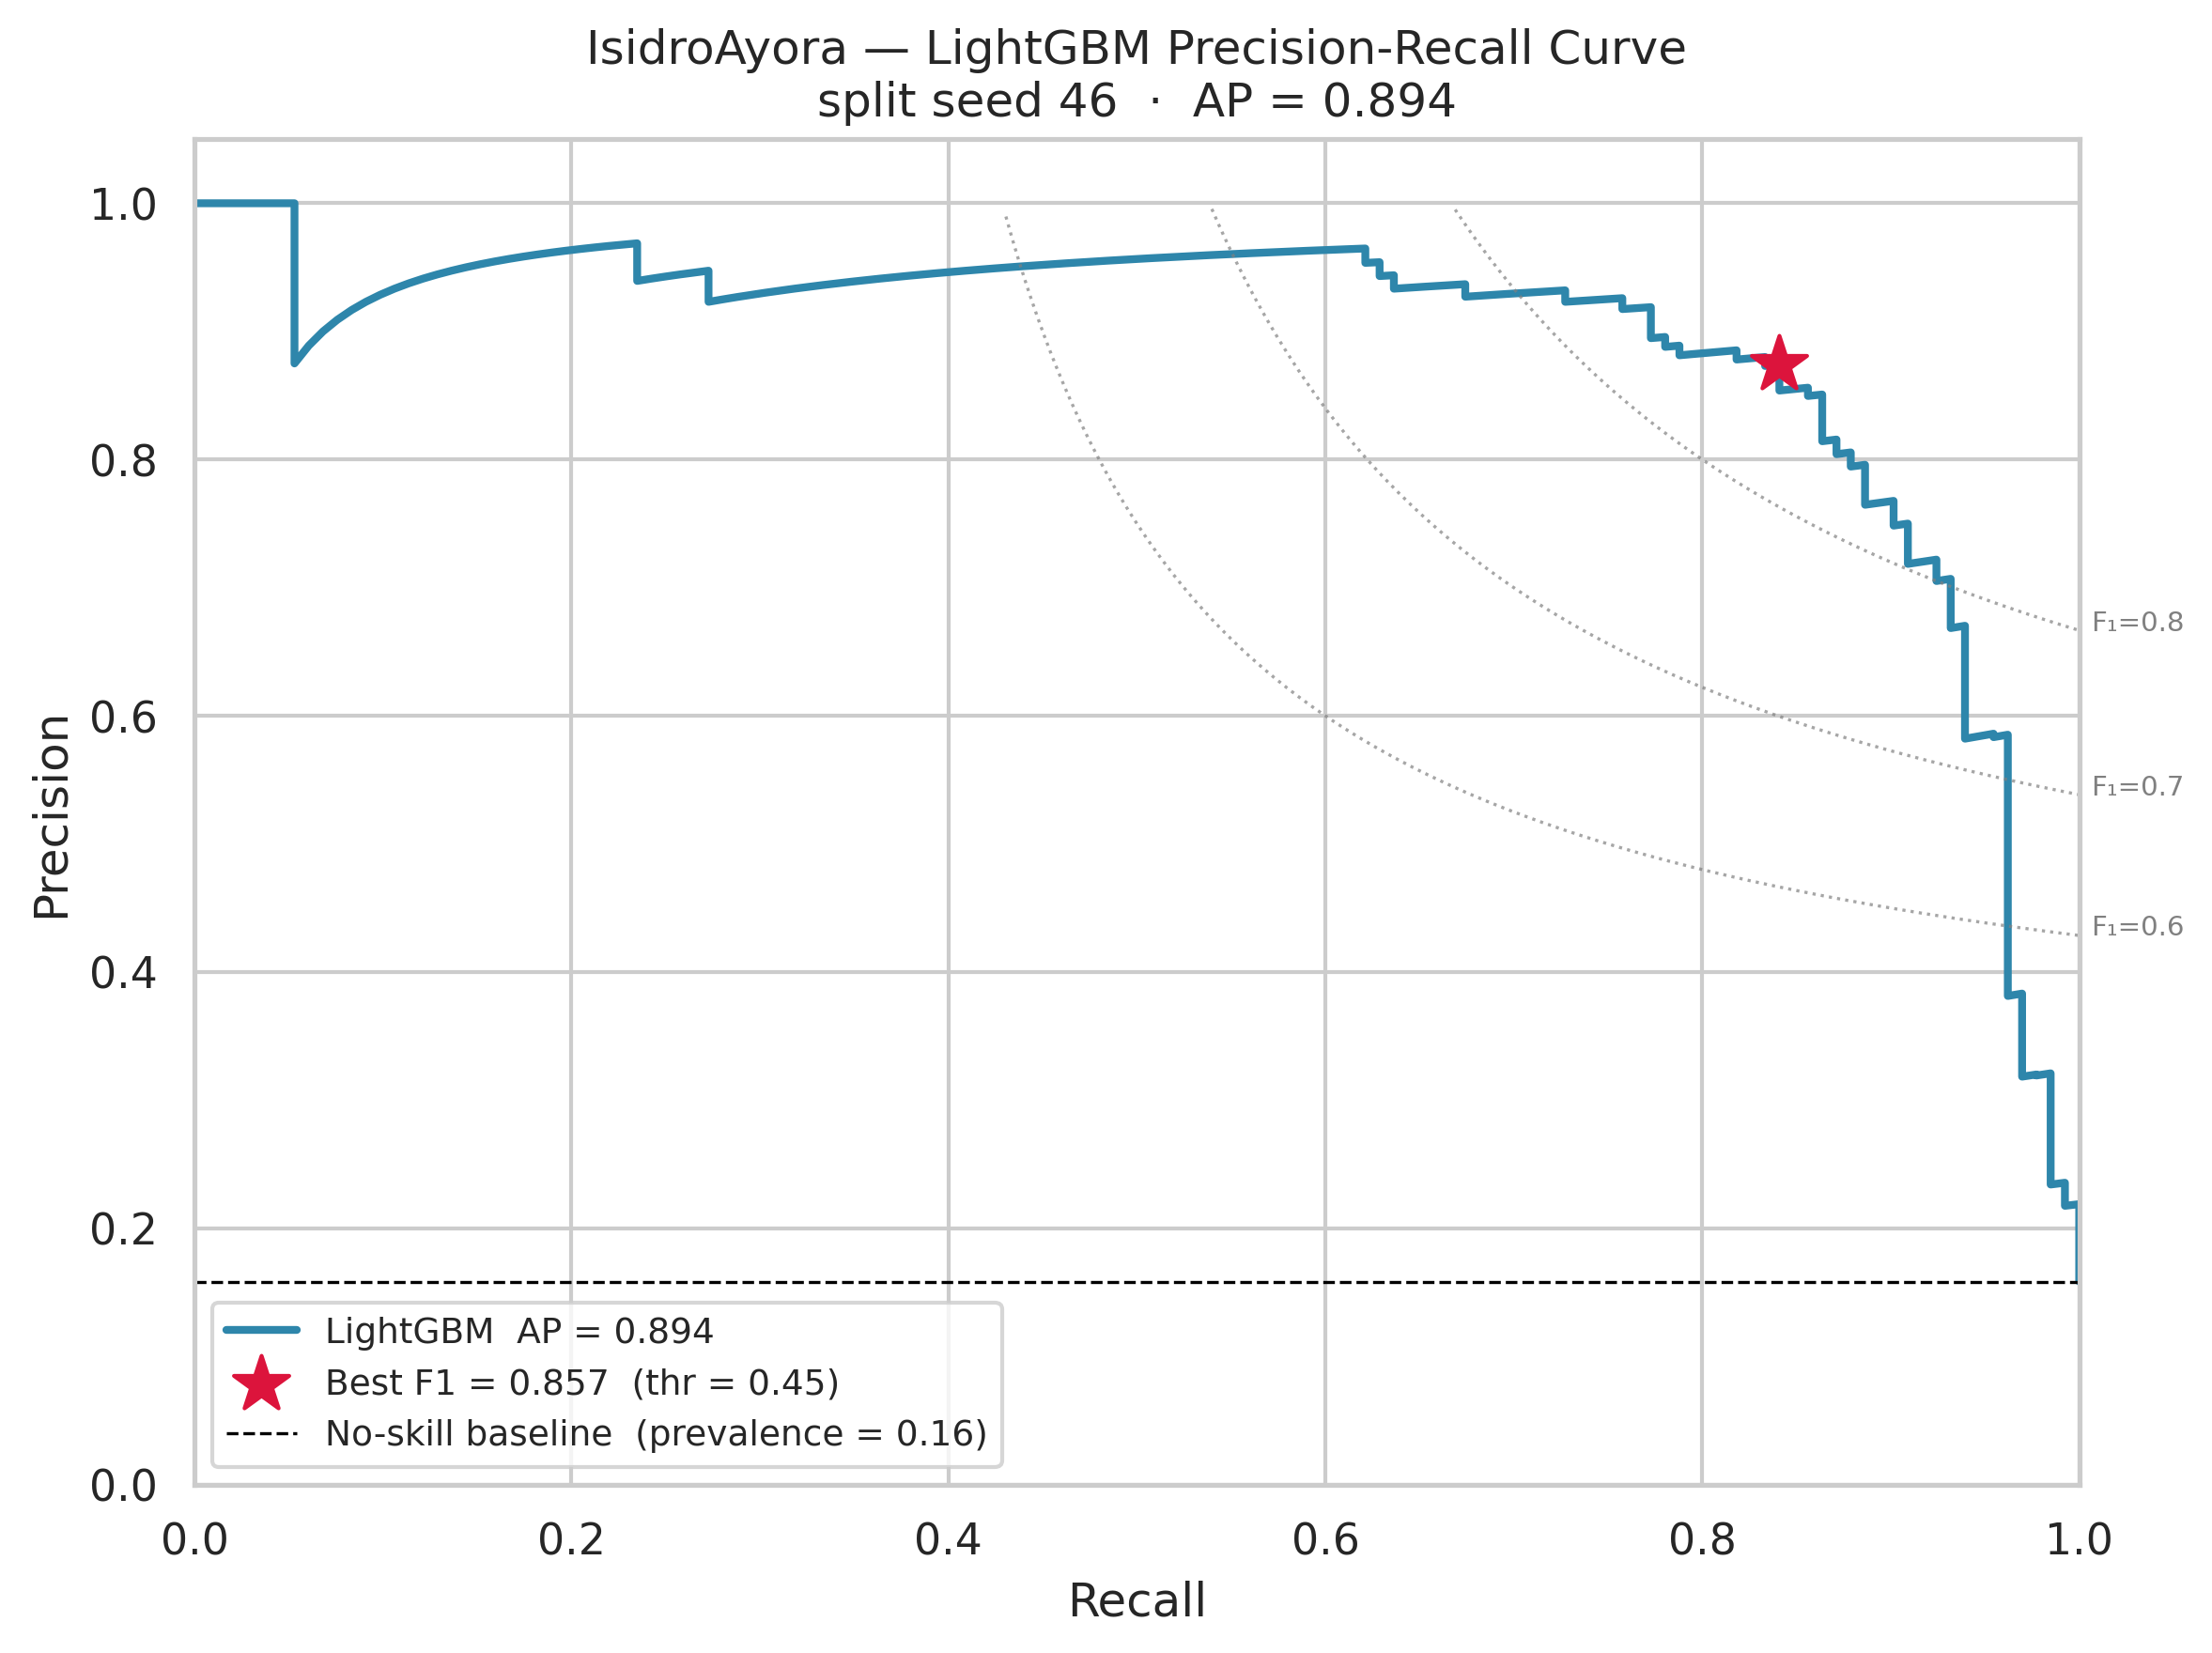
\includegraphics[width=0.48\fulllength]{figures/isidroayora_lightgbm_precision_recall_curve.png}}
\subfloat[\centering\label{fig:f1-score-models-isidro-ayora}]{
  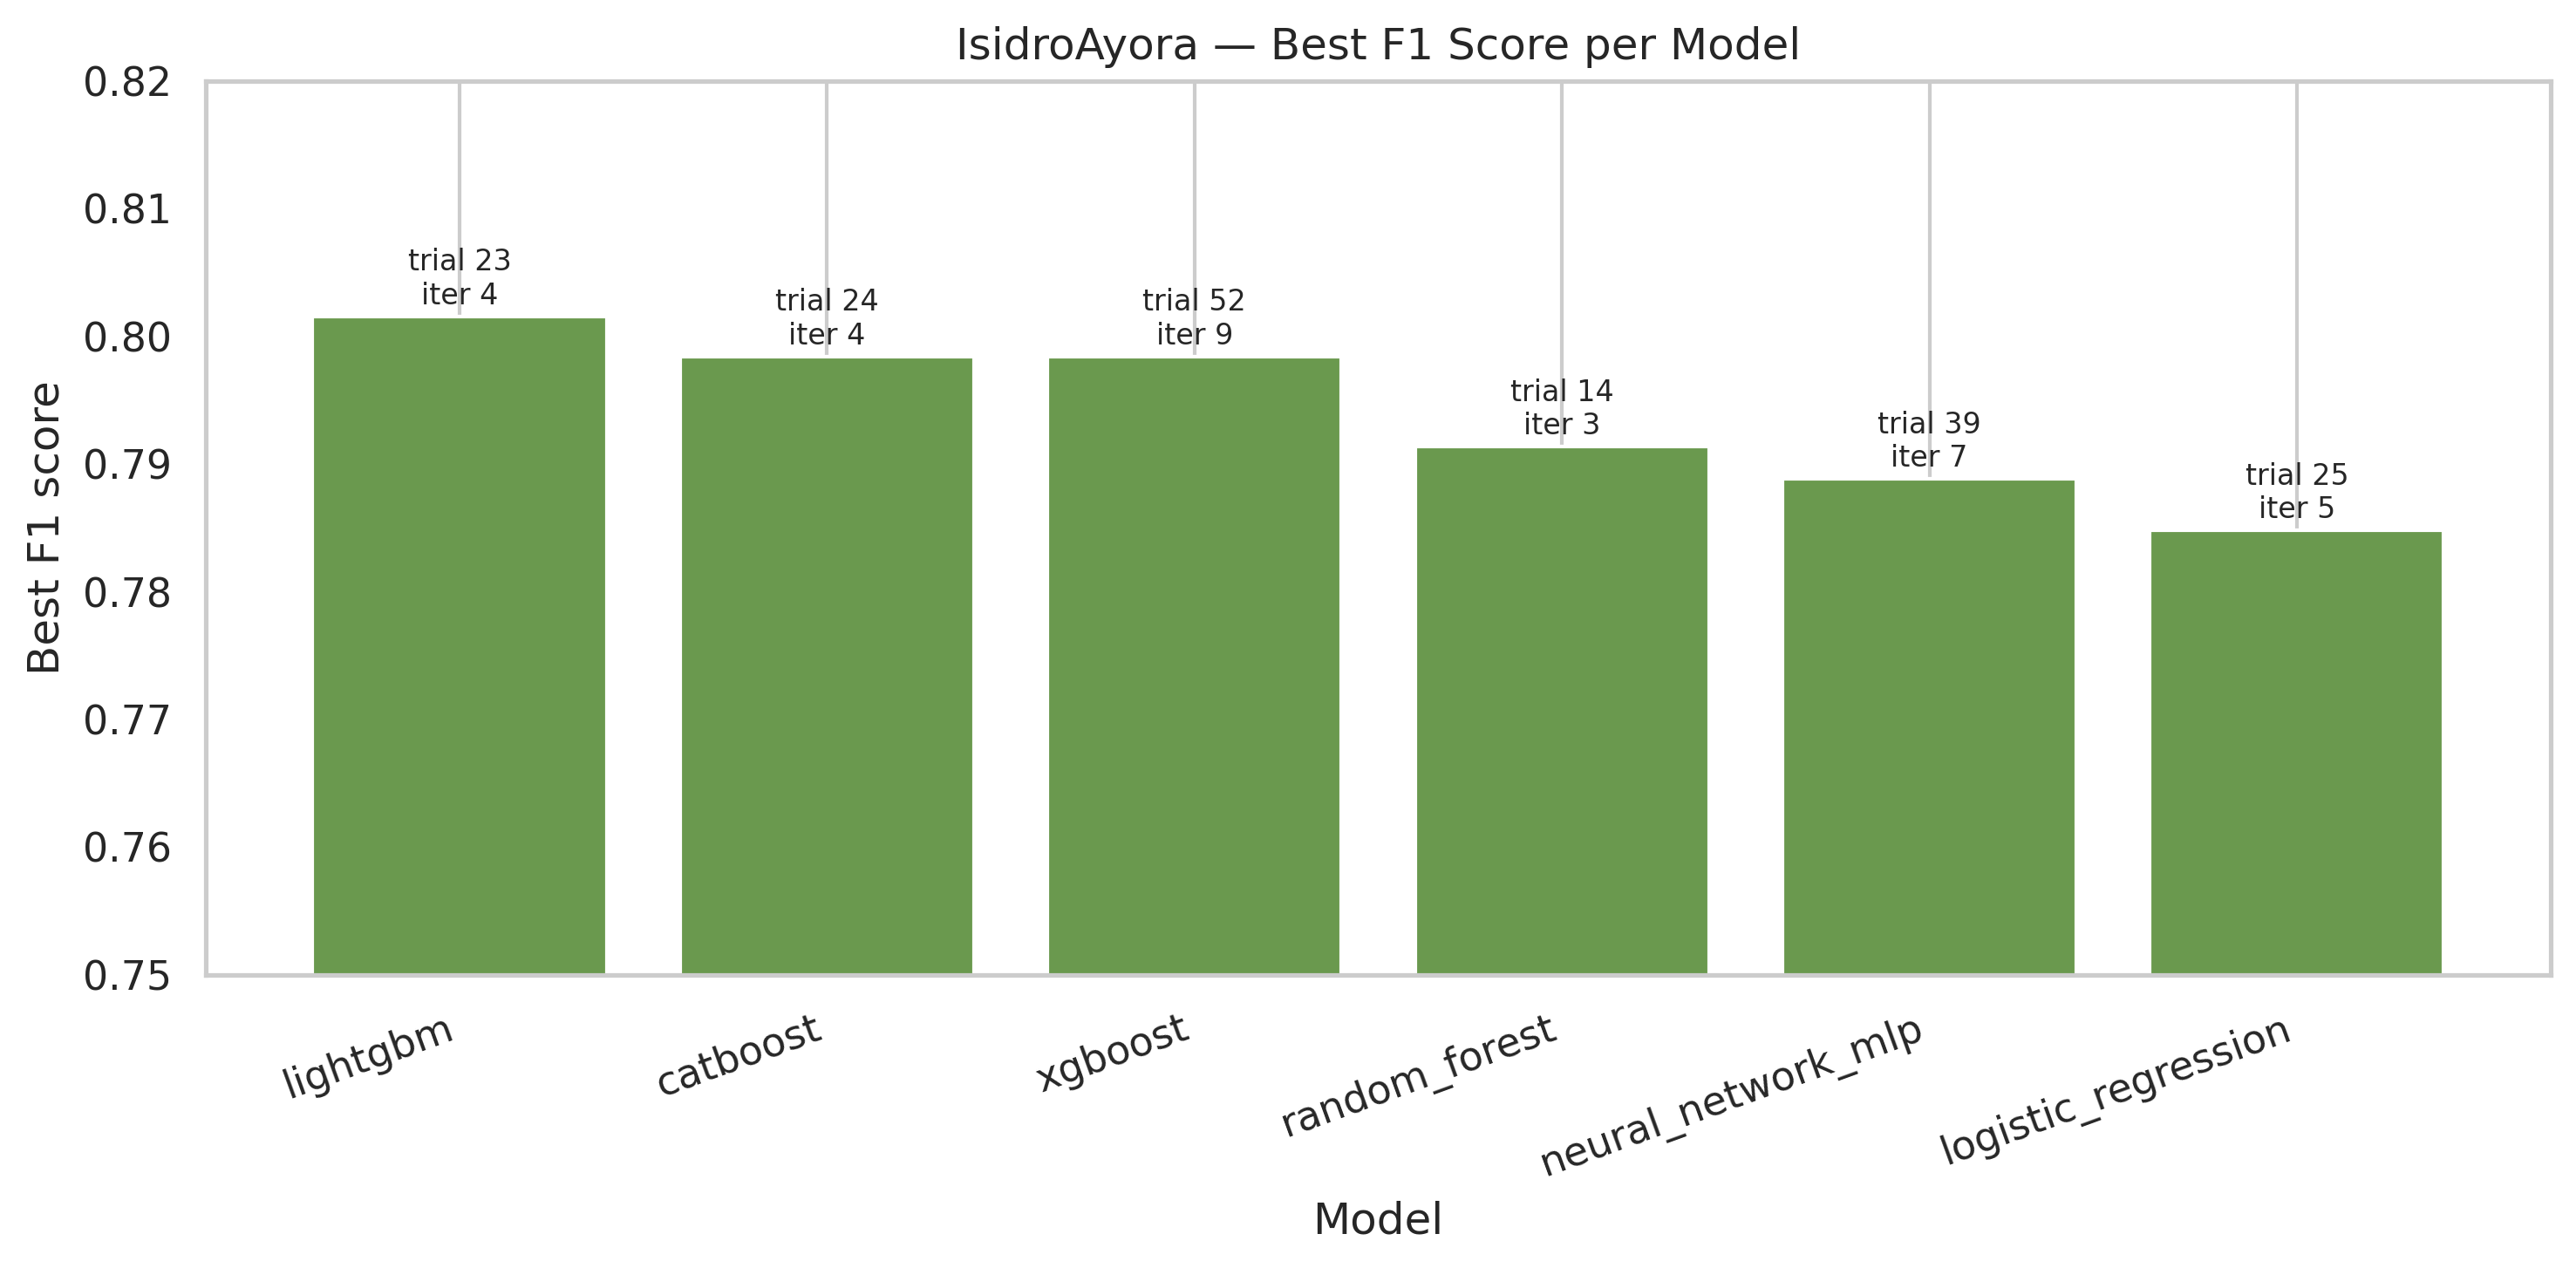
\includegraphics[width=0.48\fulllength]{figures/isidroayora_models_best_f1.png}}
\end{adjustwidth}
\caption{Performance analysis of the best C-AutoML model (LightGBM,
  Trial~23) on the \ac{HGOIA} dataset. {(\textbf{a}) Normalized
  confusion matrix.
  (\textbf{b}) Feature importance (mean $\pm$ std). (\textbf{c})
  Precision--recall curve. (\textbf{d})
  F1-score comparison across the best model from each family.} %MDPI: We moved the subfigure explanations into the figure
            %caption. Please confirm. Same with all this format
            %<<AUTHORS: Confirmed. We integrated the subfigure descriptions into one concise main caption, removed repeated wording, and retained the key details for each panel (a-d).>>
  \label{fig:combined-model-analysis-isidro-ayora}}
\end{figure}

\vspace{-9pt}


\begin{table}[H]
\caption{C-AutoML performance across trials and iterations on the
  \ac{HGOIA} dataset. Each trial uses a different
  train/validation split and hyperparameter
  configuration.\label{tab:cautoml-performance}}
%\small
\begin{tabularx}{\linewidth}{LlLCCCCC}
\toprule



%%%%%%%%%%%%%%%%%%%%% Long Table improved by Sonnet 4.6 %%%%%%%%%%%%%%%%%%%%


\textbf{Trial} & \textbf{Iter} & \textbf{Model} &
\textbf{F1} & \textbf{Acc} & \textbf{Prec} & \textbf{Rec} & \textbf{AUC} \\
\midrule





1  & 1  & LR       & 0.7344 & 0.9184 & 0.7705 & 0.7015 & 0.9318 \\
2  & 1  & RF       & 0.7368 & 0.9220 & 0.8053 & 0.6791 & 0.9341 \\
3  & 1  & MLP      & 0.7410 & 0.9220 & 0.7949 & 0.6940 & 0.9044 \\
4  & 1  & XGBoost  & 0.7431 & 0.9220 & 0.7899 & 0.7015 & 0.9384 \\
5  & 1  & LightGBM & 0.7120 & 0.9136 & 0.7672 & 0.6642 & 0.9274 \\
6  & 1  & CatBoost & 0.7460 & 0.9232 & 0.7966 & 0.7015 & 0.9393 \\
7  & 2  & LR       & 0.7417 & 0.9256 & 0.8396 & 0.6642 & 0.9467 \\
8  & 2  & RF       & 0.7713 & 0.9196 & 0.7107 & 0.8433 & 0.9506 \\
9  & 2  & MLP      & 0.7739 & 0.9292 & 0.7953 & 0.7537 & 0.9381 \\
10 & 2  & XGBoost  & 0.7786 & 0.9304 & 0.7969 & 0.7612 & 0.9558 \\
11 & 2  & LightGBM & 0.7790 & 0.9292 & 0.7820 & 0.7761 & 0.9535 \\
12 & 2  & CatBoost & 0.7510 & 0.9244 & 0.7983 & 0.7090 & 0.9525 \\
13 & 3  & LR       & 0.7296 & 0.9004 & 0.6474 & 0.8358 & 0.9482 \\
14 & 3  & RF       & 0.7914 & 0.9304 & 0.7639 & 0.8209 & 0.9421 \\
15 & 3  & MLP      & 0.7405 & 0.9184 & 0.7578 & 0.7239 & 0.9315 \\
16 & 3  & XGBoost  & 0.7382 & 0.9268 & 0.8687 & 0.6418 & 0.9478 \\
17 & 3  & LightGBM & 0.7667 & 0.9328 & 0.8679 & 0.6866 & 0.9425 \\
18 & 3  & CatBoost & 0.7809 & 0.9340 & 0.8376 & 0.7313 & 0.9472 \\
19 & 4  & LR       & 0.7121 & 0.8884 & 0.6085 & 0.8582 & 0.9428 \\
20 & 4  & RF       & 0.7557 & 0.9100 & 0.6705 & 0.8657 & 0.9436 \\
21 & 4  & MLP      & 0.7871 & 0.9364 & 0.8522 & 0.7313 & 0.9459 \\
22 & 4  & XGBoost  & 0.7795 & 0.9328 & 0.8250 & 0.7388 & 0.9362 \\
23 & 4  & \textbf{LightGBM} & \textbf{0.8016} & \textbf{0.9388} & \textbf{0.8374} & \textbf{0.7687} & \textbf{0.9443} \\
24 & 4  & CatBoost & 0.7984 & 0.9388 & 0.8487 & 0.7537 & 0.9462 \\
25 & 5  & LR       & 0.7848 & 0.9388 & 0.9029 & 0.6940 & 0.9478 \\
26 & 5  & RF       & 0.7389 & 0.9016 & 0.6444 & 0.8657 & 0.9512 \\
27 & 5  & MLP      & 0.7805 & 0.9352 & 0.8571 & 0.7164 & 0.9443 \\
28 & 5  & XGBoost  & 0.7938 & 0.9364 & 0.8293 & 0.7612 & 0.9553 \\
29 & 5  & LightGBM & 0.7755 & 0.9340 & 0.8559 & 0.7090 & 0.9469 \\
30 & 5  & CatBoost & 0.7791 & 0.9340 & 0.8435 & 0.7239 & 0.9453 \\
31 & 6  & LR       & 0.7101 & 0.8932 & 0.6301 & 0.8134 & 0.9338 \\
32 & 6  & RF       & 0.7311 & 0.9232 & 0.8365 & 0.6493 & 0.9418 \\
33 & 6  & MLP      & 0.7511 & 0.9292 & 0.8641 & 0.6642 & 0.9327 \\
34 & 6  & XGBoost  & 0.7531 & 0.9292 & 0.8571 & 0.6716 & 0.9457 \\
35 & 6  & LightGBM & 0.7542 & 0.9304 & 0.8725 & 0.6642 & 0.9439 \\
36 & 6  & CatBoost & 0.7667 & 0.9328 & 0.8679 & 0.6866 & 0.9396 \\
37 & 7  & LR       & 0.7147 & 0.8860 & 0.5980 & 0.8881 & 0.9457 \\
38 & 7  & RF       & 0.7758 & 0.9244 & 0.7415 & 0.8134 & 0.9478 \\
39 & 7  & MLP      & 0.7888 & 0.9364 & 0.8462 & 0.7388 & 0.9526 \\
40 & 7  & XGBoost  & 0.7667 & 0.9328 & 0.8679 & 0.6866 & 0.9495 \\
41 & 7  & LightGBM & 0.7668 & 0.9292 & 0.8151 & 0.7239 & 0.9506 \\
42 & 7  & CatBoost & 0.7843 & 0.9340 & 0.8264 & 0.7463 & 0.9535 \\
43 & 8  & LR       & 0.7186 & 0.9220 & 0.8557 & 0.6194 & 0.9383 \\
44 & 8  & RF       & 0.7450 & 0.9088 & 0.6768 & 0.8284 & 0.9418 \\
45 & 8  & MLP      & 0.7529 & 0.9244 & 0.7934 & 0.7164 & 0.9352 \\
46 & 8  & XGBoost  & 0.7339 & 0.9208 & 0.7982 & 0.6791 & 0.9386 \\
47 & 8  & LightGBM & 0.7243 & 0.9196 & 0.8073 & 0.6567 & 0.9397 \\
48 & 8  & CatBoost & 0.7360 & 0.9208 & 0.7931 & 0.6866 & 0.9296 \\
49 & 9  & LR       & 0.7107 & 0.8896 & 0.6141 & 0.8433 & 0.9419 \\
50 & 9  & RF       & 0.7550 & 0.9112 & 0.6786 & 0.8507 & 0.9444 \\
\bottomrule
\end{tabularx}


\end{table}


\begin{table}[H]\ContinuedFloat   
\caption{\emph{Cont.}\label{tab:cautoml-performance}}
\begin{tabularx}{\linewidth}{LlLCCCCC}
\toprule



%%%%%%%%%%%%%%%%%%%%% Long Table improved by Sonnet 4.6 %%%%%%%%%%%%%%%%%%%%


\textbf{Trial} & \textbf{Iter} & \textbf{Model} &
\textbf{F1} & \textbf{Acc} & \textbf{Prec} & \textbf{Rec} & \textbf{AUC} \\
\midrule




51 & 9  & MLP      & 0.7686 & 0.9292 & 0.8099 & 0.7313 & 0.9454 \\
52 & 9  & XGBoost  & 0.7984 & 0.9388 & 0.8487 & 0.7537 & 0.9448 \\
53 & 9  & LightGBM & 0.7922 & 0.9364 & 0.8347 & 0.7537 & 0.9424 \\
54 & 9  & CatBoost & 0.7860 & 0.9340 & 0.8211 & 0.7537 & 0.9418 \\
55 & 10 & LR       & 0.6894 & 0.8800 & 0.5904 & 0.8284 & 0.9349 \\
56 & 10 & RF       & 0.7666 & 0.9196 & 0.7190 & 0.8209 & 0.9398 \\
57 & 10 & MLP      & 0.7317 & 0.9208 & 0.8036 & 0.6716 & 0.9370 \\
58 & 10 & XGBoost  & 0.7347 & 0.9220 & 0.8108 & 0.6716 & 0.9309 \\
59 & 10 & LightGBM & 0.7137 & 0.9172 & 0.8037 & 0.6418 & 0.9359 \\
60 & 10 & CatBoost & 0.7540 & 0.9256 & 0.8051 & 0.7090 & 0.9341 \\
\bottomrule
\end{tabularx}
\noindent{\footnotesize{Abbreviations---LR: Logistic Regression;
    RF: Random Forest; MLP: Multi-Layer Perceptron; XGBoost: Extreme
    Gradient Boosting; LightGBM: Light Gradient Boosting Machine;
    CatBoost: Categorical Boosting. \textbf{Bold} row indicates the
    best-performing model overall.}}

\end{table}
 
 

\subsection{Performance of Weighted Ensemble Model on \ac{HGOIA} Data}
\label{sec:performance-aws-sage-maker-canvas}

Table~\ref{tab:canvas-model-performance} summarizes the performance of
the different models evaluated in Amazon SageMaker Canvas. The best
performance was achieved by the Weighted Ensemble Model.
Inspection of the downloaded model artifact confirmed
  that the ensemble comprised three base models selected with equal
  weights ($w_k = \tfrac{1}{3}$, Equation~\eqref{eq:ensemble-prediction}):
  LightGBM, Random Forest (Entropy), and NeuralNetFastAI; the
  remaining seven Layer~1 candidates did not improve validation
  \ac{F1} and were excluded. The ensemble achieved
$\mathrm{F1}=0.805$, $\mathrm{Precision}=0.770$, $\mathrm{Recall}=0.844$, and
$\mathrm{AUC}=0.956$. Compared to the LightGBM model trained with
our proposed \ac{C-AutoML}, the AWS model improves on the recall
performance metric, reducing the number of false negatives. However,
the precision of the LightGBM model implies a smaller
false-positive rate, which translates into fewer examinations.


%%%%%%%%%%%%%%%%%%%% Normal Table %%%%%%%%%%%%%%%%%%%%
% the normal table option can be consulted at
% https://claude.ai/chat/ebafc645-192b-413c-aeeb-f0e24a8a396e in case
% asked to reformat
%%%%%%%%%%%%%%%%%%%% wide table %%%%%%%%%%%%%%%%%%%%

\begin{table}[H]
\caption{Performance of models evaluated in Amazon SageMaker Canvas.
  \textbf{Bold} row indicates the default (best) model selected by
  Canvas.\label{tab:canvas-model-performance}}
\begin{adjustwidth}{-\extralength}{0cm}
\small
\begin{tabularx}{\fulllength}{>{\raggedright\arraybackslash}p{3.5cm}
  *{8}{>{\centering\arraybackslash}X}}
\toprule
\textbf{Model Prefix} \textbf{\textsuperscript{\dag}} & \textbf{F1 (\%)} &
\textbf{Acc (\%)} & \textbf{AUC} & \textbf{Bal.\ Acc (\%)} &
\textbf{Prec (\%)} & \textbf{Rec (\%)} & \textbf{Log Loss} &
\textbf{Latency (s)} \\
\midrule
\textbf{\texttt{FULL-t4785127992329}} {(default)} %MDPI: Please add
                                %an explanation for the use of italics
                                %in the table footer. If the italics
                                %is unnecessary, please remove it. The
                                %following highlights are the
                                %same.<<AUTHORS: removed italics as suggested>>
  & \textbf{80.565} & \textbf{93.405} & \textbf{0.956} & \textbf{89.790} & \textbf{77.027} & \textbf{84.444} & \textbf{0.210} & \textbf{0.162} \\
\texttt{FULL-t9785127992329}
  & 78.388 & 92.926 & 0.954 & 87.412 & 77.536 & 79.259 & 0.193 & 0.178 \\
\texttt{FULL-t8785127992329}
  & 80.565 & 93.405 & 0.956 & 89.790 & 77.027 & 84.444 & 0.210 & 0.184 \\
\texttt{FULL-t7785127992329}
  & 79.310 & 92.806 & 0.955 & 89.731 & 74.194 & 85.185 & 0.225 & 0.321 \\
\texttt{FULL-t6785127992329}
  & 77.124 & 91.607 & 0.957 & 89.913 & 69.006 & 87.407 & 0.269 & 0.094 \\
\texttt{FULL-t5785127992329}
  & 80.000 & 93.165 & 0.956 & 89.647 & 76.000 & 84.444 & 0.226 & 0.099 \\
\texttt{FULL-t2785127992329}
  & 79.298 & 92.926 & 0.956 & 89.205 & 75.333 & 83.704 & 0.211 & 0.207 \\
\texttt{FULL-t1785127992329}
  & 80.565 & 93.405 & 0.956 & 89.790 & 77.027 & 84.444 & 0.210 & 0.165 \\
\texttt{FULL-t10785127992329}
  & 79.710 & 93.285 & 0.954 & 88.523 & 78.014 & 81.481 & 0.192 & 0.152 \\
\texttt{-t5785127992329}
  & 76.873 & 91.487 & 0.955 & 89.841 & 68.605 & 87.407 & 0.264 & 0.086 \\
\bottomrule
\end{tabularx}
\end{adjustwidth}
\noindent{\footnotesize{\textsuperscript{\dag} All model names share
    the common suffix \texttt{Canvas1774655537951}; full name is
    \texttt{<prefix>-Canvas1774655537951}.}}
\end{table}

Figure~\ref{fig:combined-model-analysis-isidro-ayora-aws} presents
the normalized confusion
matrix~(Figure~\ref{fig:combined-model-analysis-isidro-ayora-aws}a), the KernelSHAP values
for model interpretability~(Figure~\ref{fig:combined-model-analysis-isidro-ayora-aws}b), the
precision--recall curve performance (\mbox{Figure~\ref{fig:combined-model-analysis-isidro-ayora-aws}c)}, and
a comparison \ac{w.r.t.} the \ac{F1} of the trained models in AWS
SageMaker Canvas in (\mbox{Figure~\ref{fig:combined-model-analysis-isidro-ayora-aws}d).}

\begin{figure}[H]
\begin{adjustwidth}{-\extralength}{0cm}
\centering
\subfloat[\centering \label{fig:confusion-matrix-bestmodel-aws}]{
  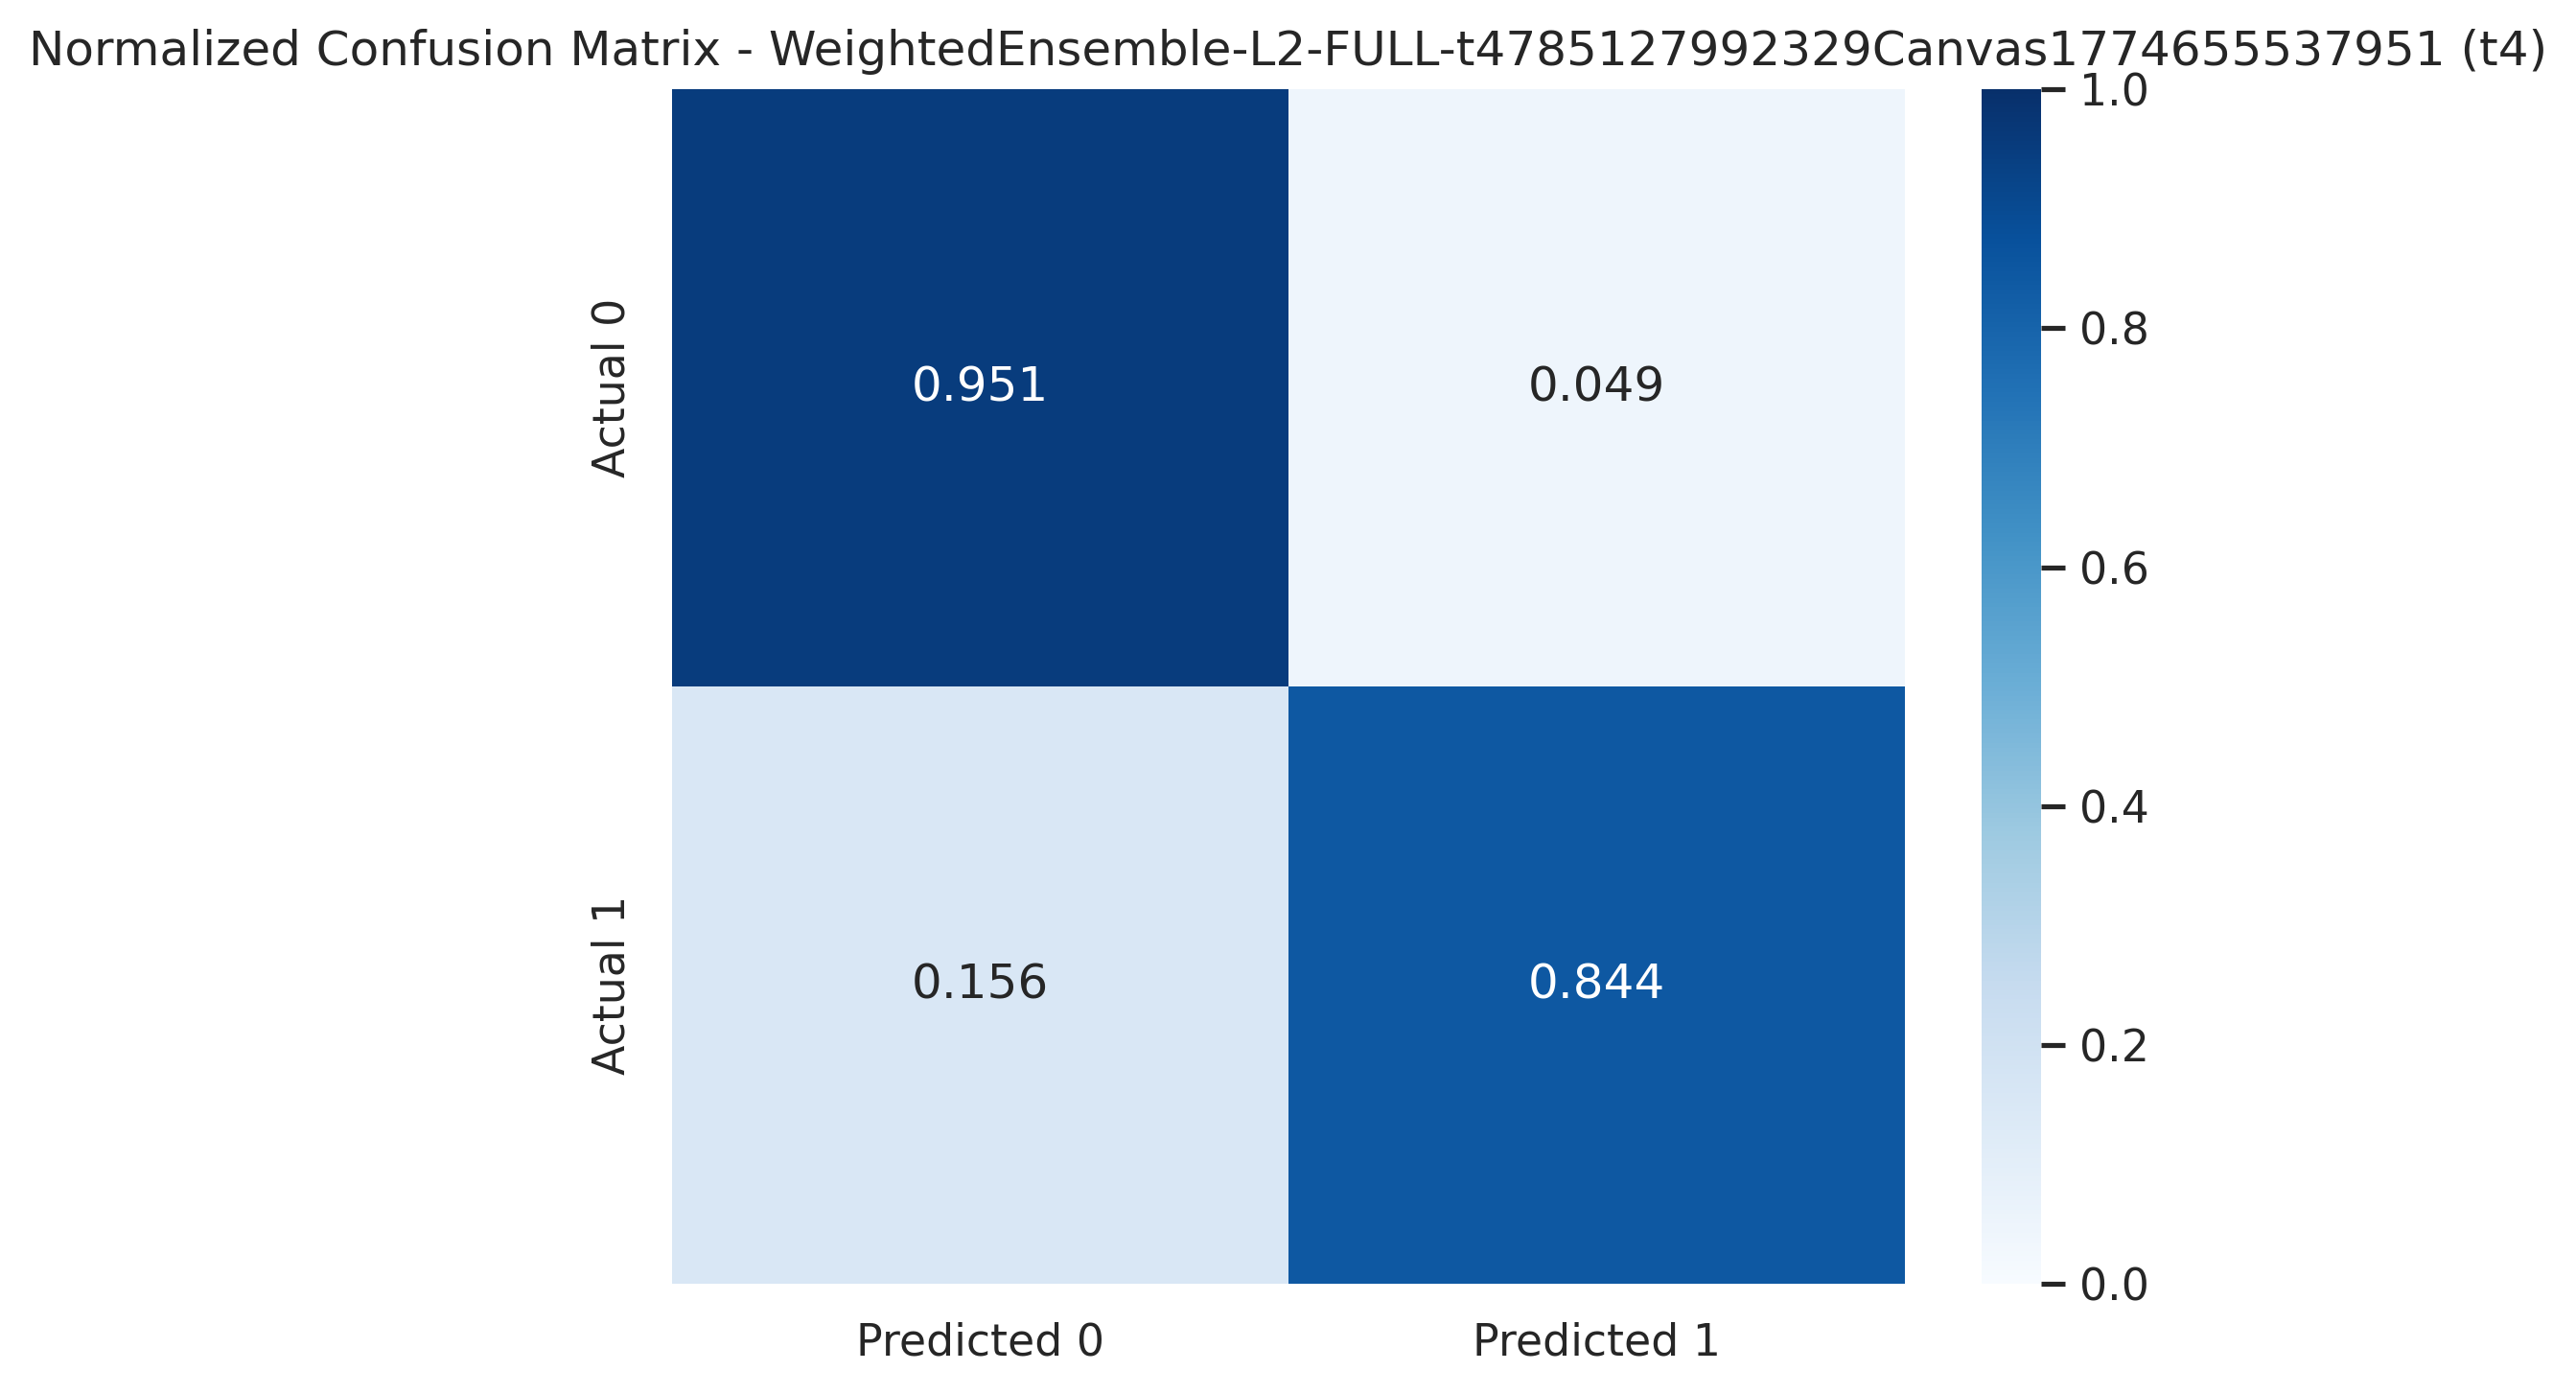
\includegraphics[width=0.48\fulllength, height=0.35\textheight, keepaspectratio]{figures/canvas_sagemaker_model_monitor/best_model_confusion_matrix_normalized.png}}
\subfloat[\centering \label{fig:feature-importance-aws}]{
  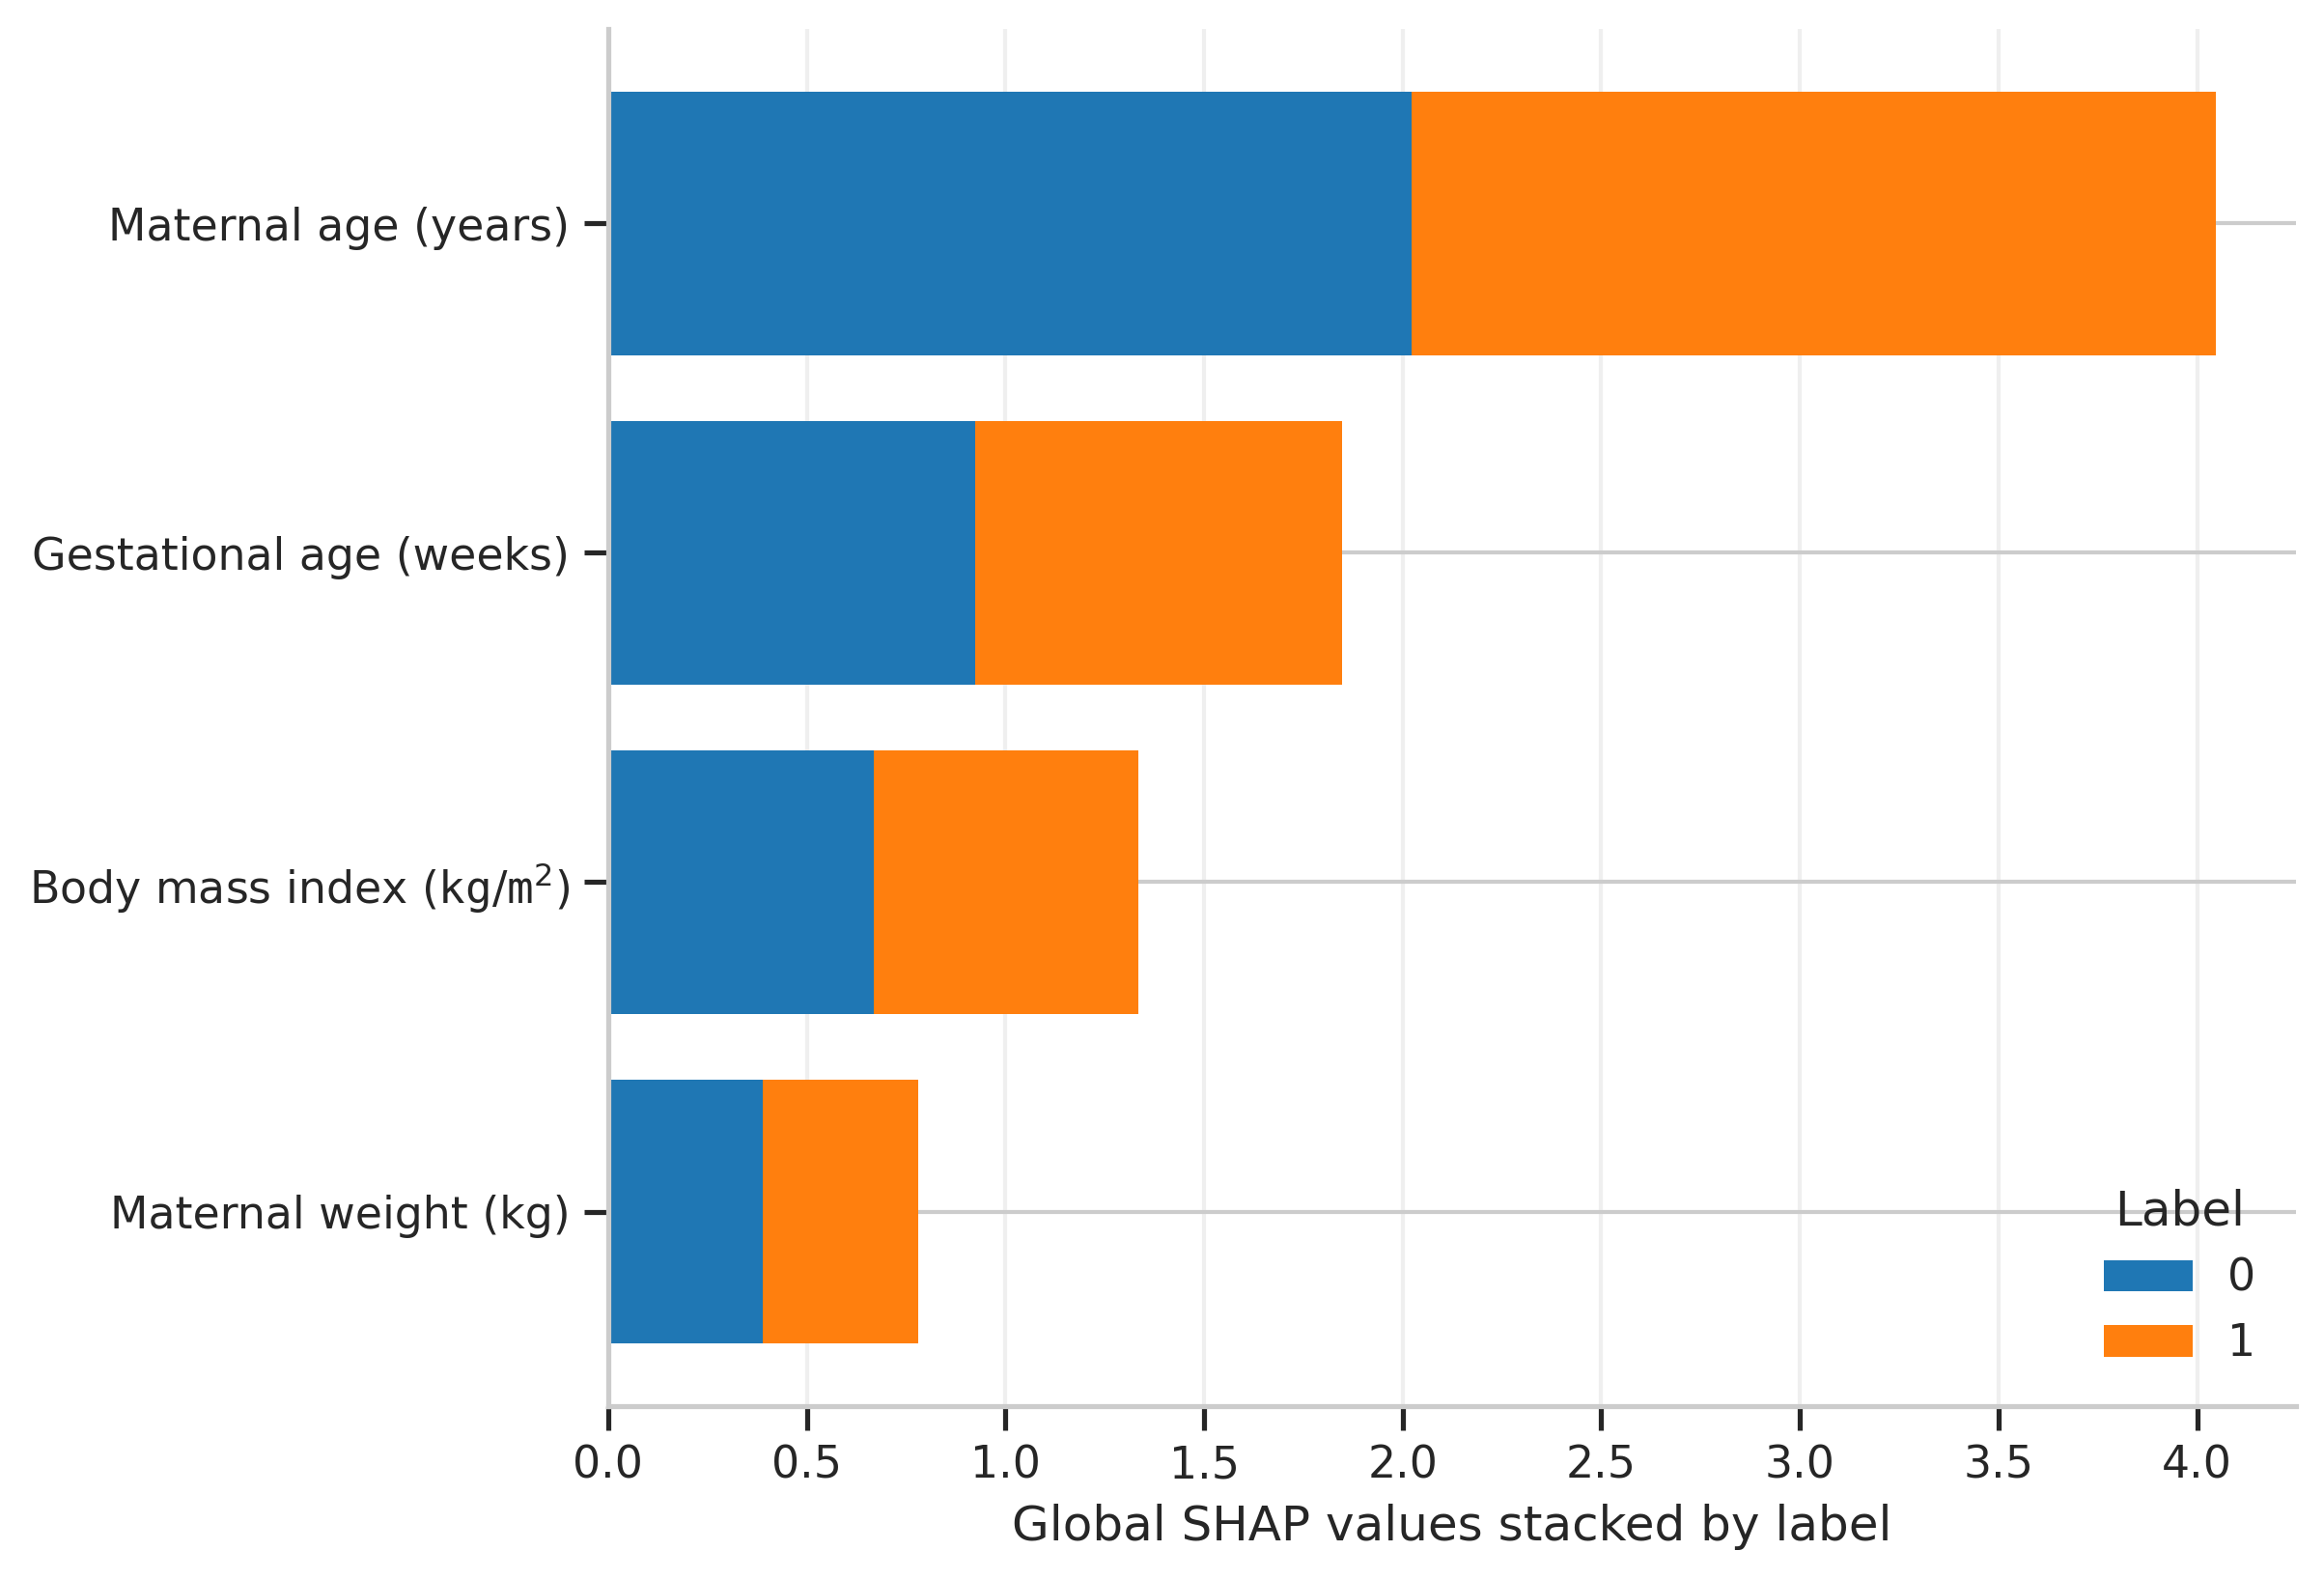
\includegraphics[width=0.48\fulllength, height=0.35\textheight, keepaspectratio]{figures/shap_explainability/canvas_sagemaker_model/canvas_global_shap_stacked_by_label.png}}\\
\subfloat[\centering \label{fig:precision-recall-aws}]{
  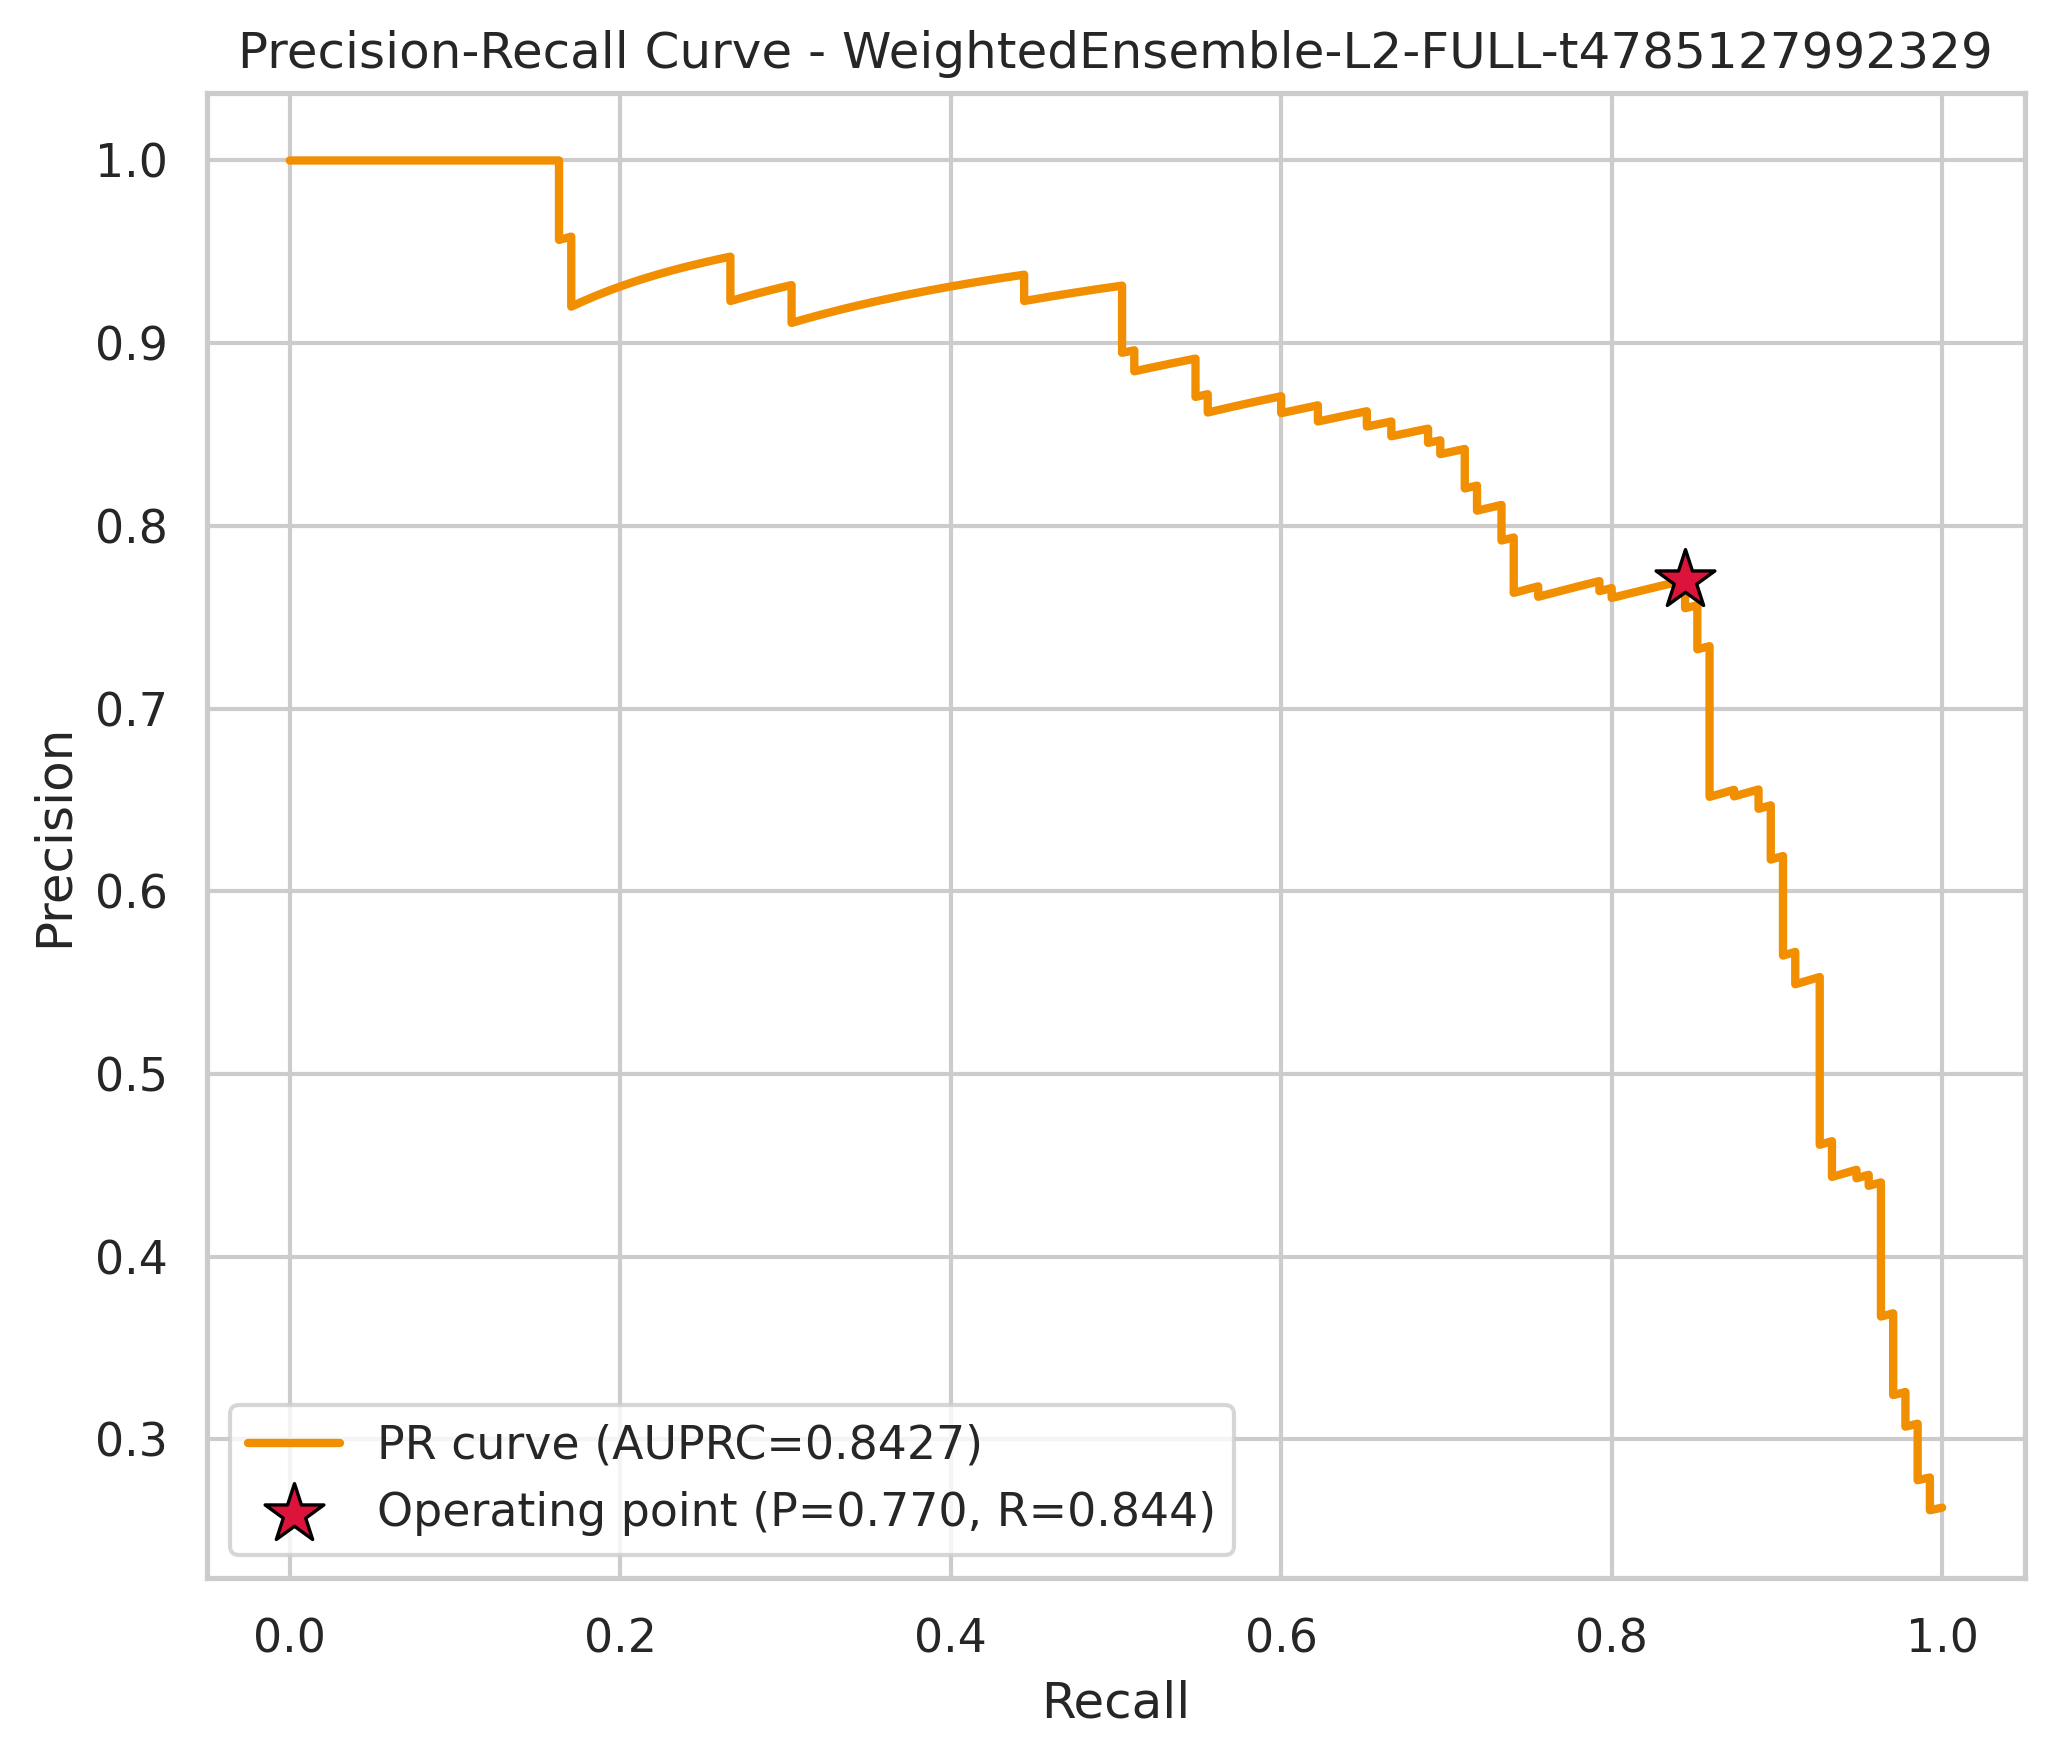
\includegraphics[width=0.48\fulllength, height=0.35\textheight, keepaspectratio]{figures/canvas_sagemaker_model_monitor/best_model_precision_recall_curve.png}}
\subfloat[\centering \label{fig:f1-score-models-isidro-ayora-aws}]{
  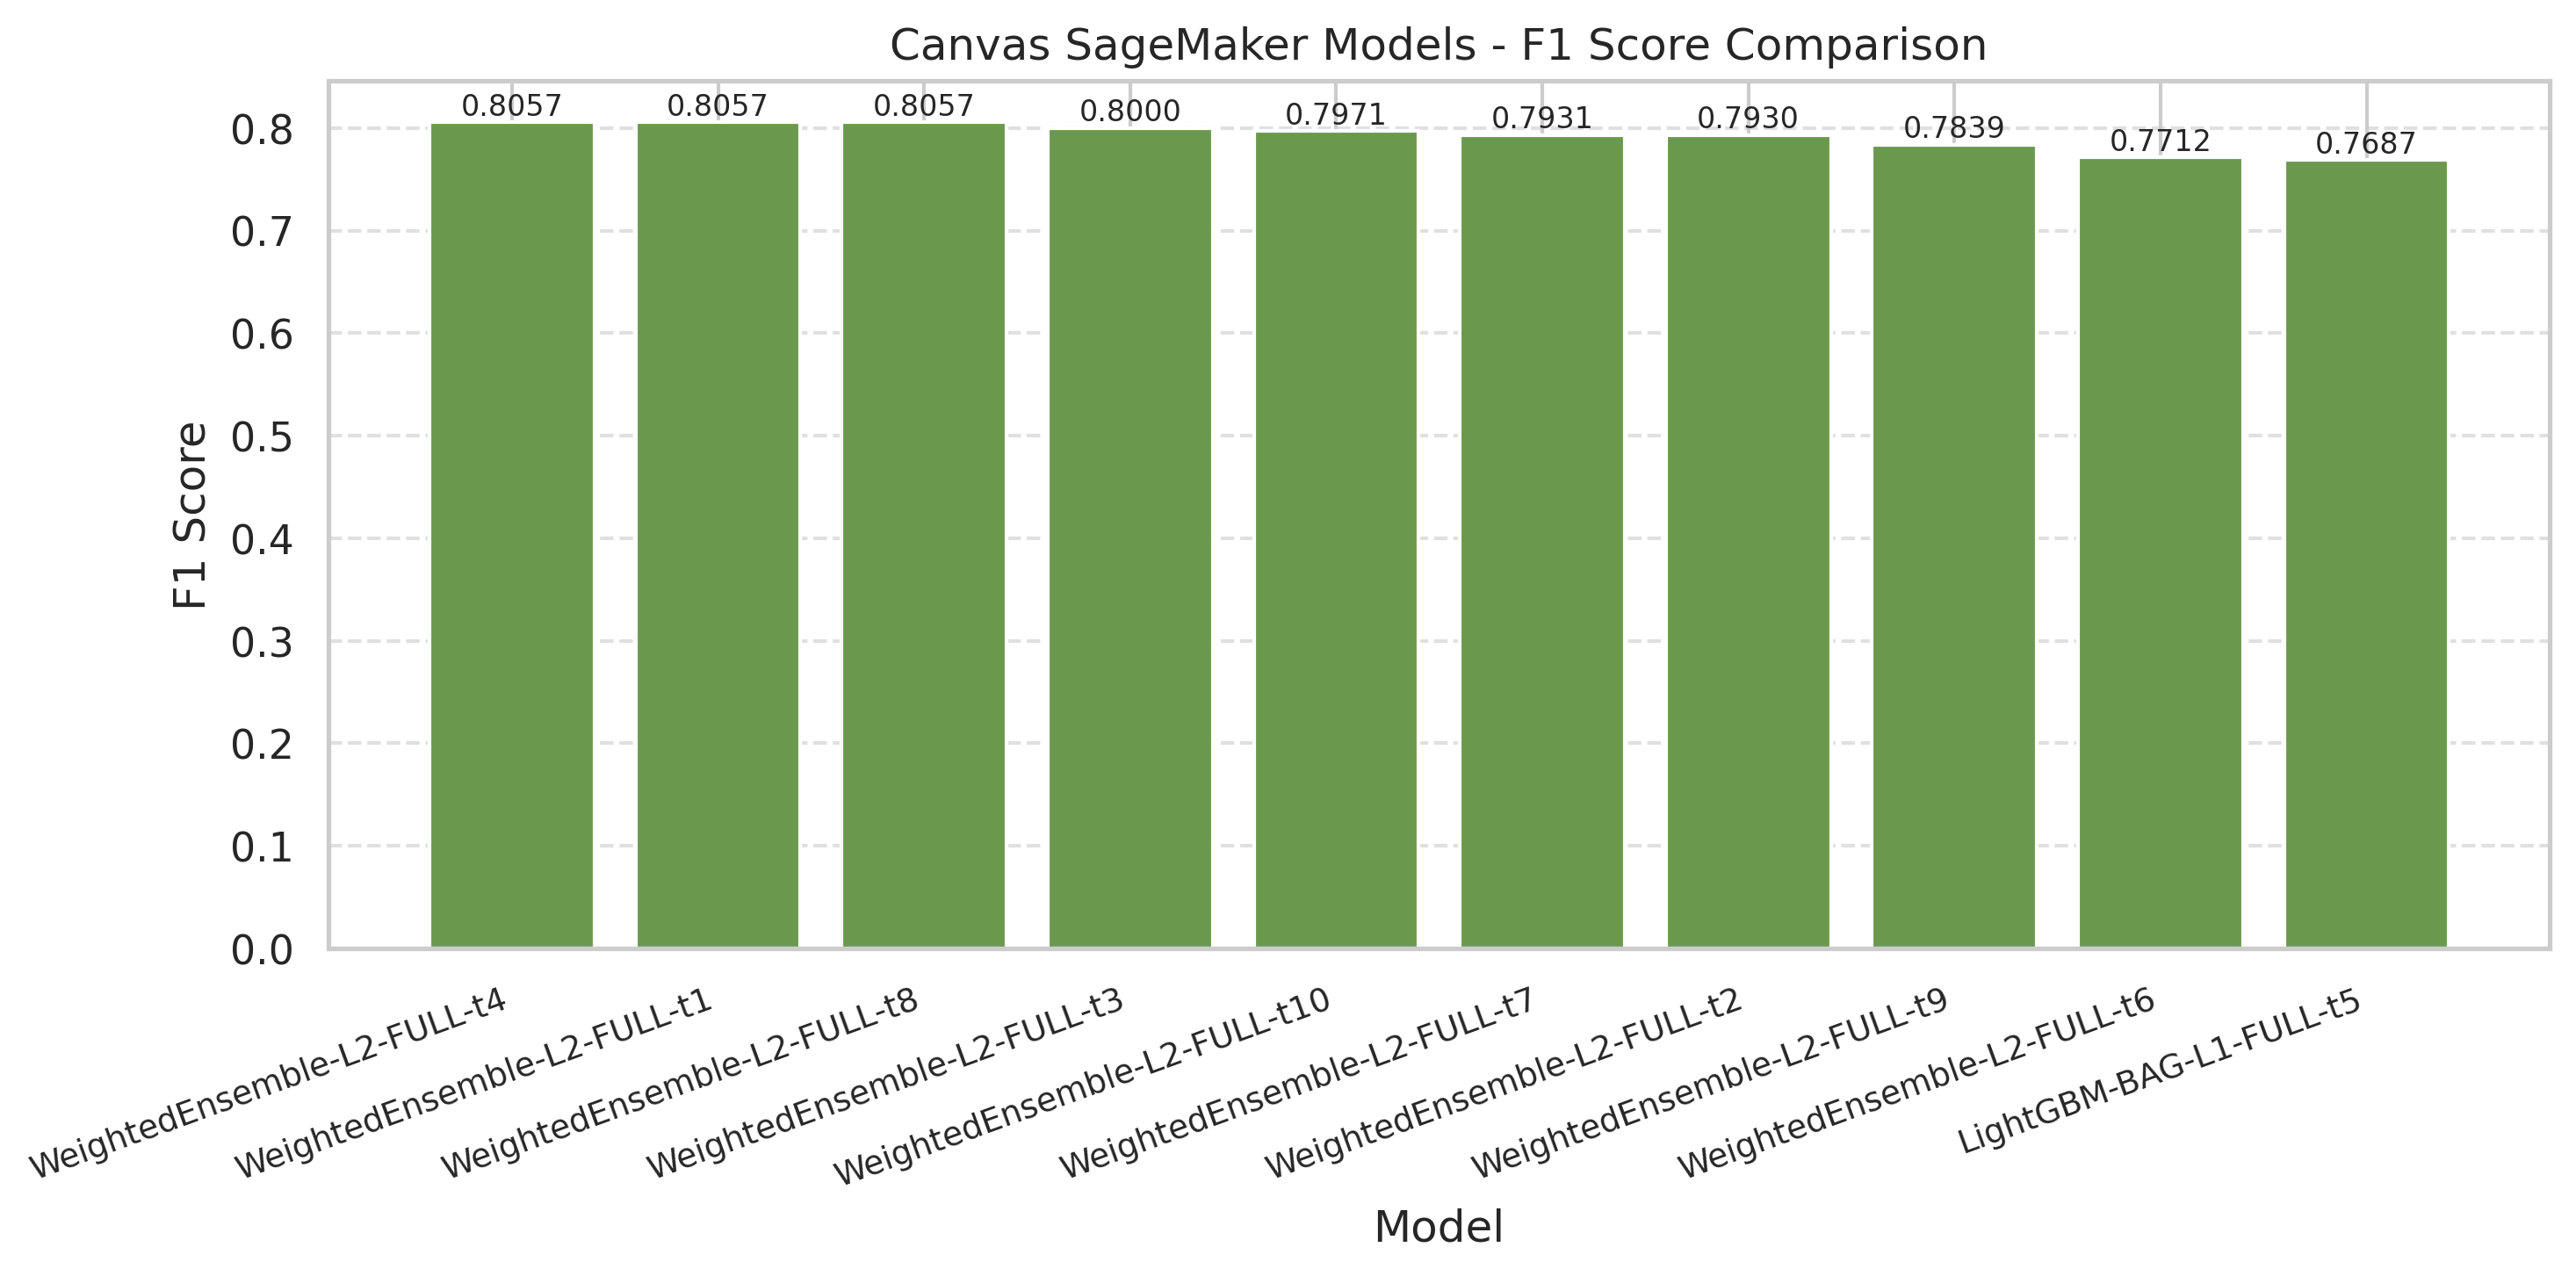
\includegraphics[width=0.48\fulllength, height=0.35\textheight, keepaspectratio]{figures/canvas_sagemaker_model_monitor/all_models_f1_comparison.png}}
\end{adjustwidth}
\caption{{Performance} analysis of the Amazon SageMaker Canvas Weighted
  Ensemble on the \ac{HGOIA} dataset. (\textbf{a})  Normalized confusion matrix. (\textbf{b})  KernelSHAP feature importance values for the Amazon SageMaker
  Weighted Ensemble. (\textbf{c})  Precision--recall curve for the Amazon SageMaker Weighted
  Ensemble model. (\textbf{d}) F1-score comparison across all models trained in Amazon
  SageMaker Canvas. % <<AUTHORS: we removed redundant writing>>
  \label{fig:combined-model-analysis-isidro-ayora-aws}}
\end{figure}

\subsection{Logistic Regression Model on Clinical Synthetic Generated Data}
\label{sec:synth-data-results}
In this case, our proposed methodology \ac{C-AutoML} achieved its best
performance for model \ac{LR}, with a perfect score of $\mathrm{F1}=1.000$
on Trial\#1,
iteration\#1. Table~\ref{tab:cautoml-synthetic-performance} presents
the complete performance of the different trials for each of the
proposed models and iterations. It should be noted that more than one
model achieves a similar performance score as \ac{LR} for the
synthetic data. This is structurally expected: the diagnostic
label $\mathrm{PE}_{\mathrm{MSP}}$ is assigned by the deterministic
threshold rule in Equation~\eqref{eq:preeclampsia-msp-rule}, which
applies linear inequality conditions to the same features used as model
inputs, producing linearly separable class boundaries that any of the
evaluated classifiers can recover. The consistently near-perfect
scores therefore confirm that the parametric distributions in
Table~\ref{tab:distributions} are sufficiently separated with respect to
the \ac{MSP} rule, validating the generation process itself.

Figure~\ref{fig:combined-model-analysis-synthetic} presents the
performance of the \ac{LR} model according with the normalized
confusion matrix (Figure~\ref{fig:combined-model-analysis-synthetic}a), the
feature importance values
(Figure~\ref{fig:combined-model-analysis-synthetic}b), the precision--recall
curve (Figure~\ref{fig:combined-model-analysis-synthetic}c), and a comparison
of the \ac{F1} among the trained
models (Figure~\ref{fig:combined-model-analysis-synthetic}d). The
feature-effects plot indicates that systolic blood pressure, platelet
count, 24 h proteinuria, and AST were the dominant contributors in
the selected \ac{LR} model, which is coherent with the
clinical rule used to generate the synthetic labels.



\begin{figure}[H]
\begin{adjustwidth}{-\extralength}{0cm}
\centering
\subfloat[\centering \label{fig:confusion-matrix-lr-synthetic}]{
  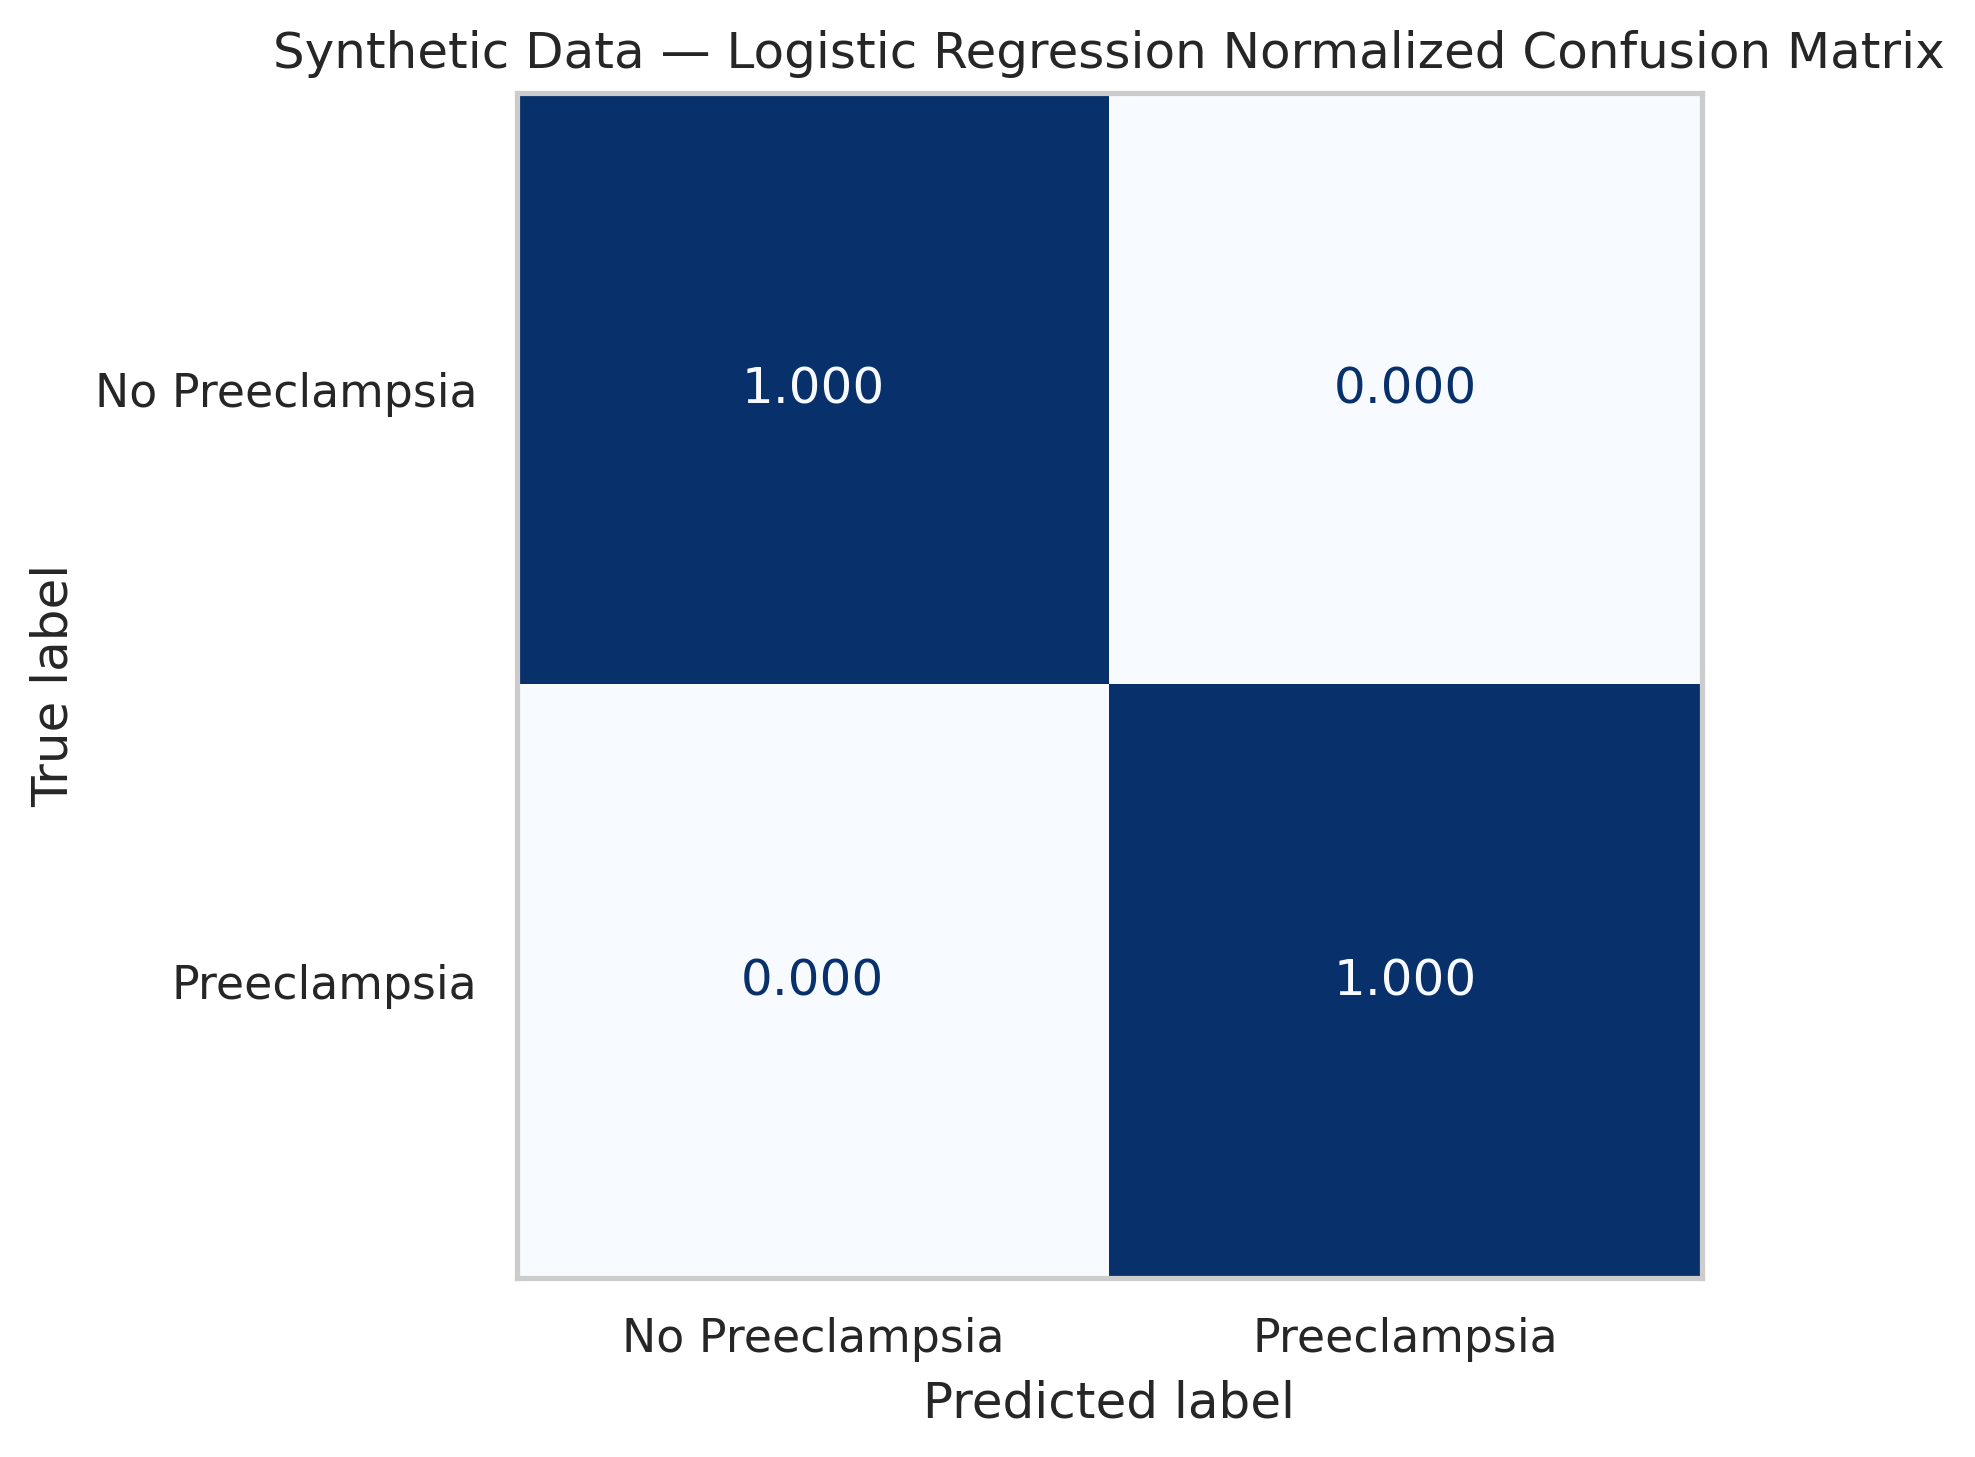
\includegraphics[width=0.48\fulllength]{figures/synthetic_logistic_regression_normalized_confusion_matrix.png}}
\subfloat[\centering \label{fig:feature-importance-lr-synthetic}]{
  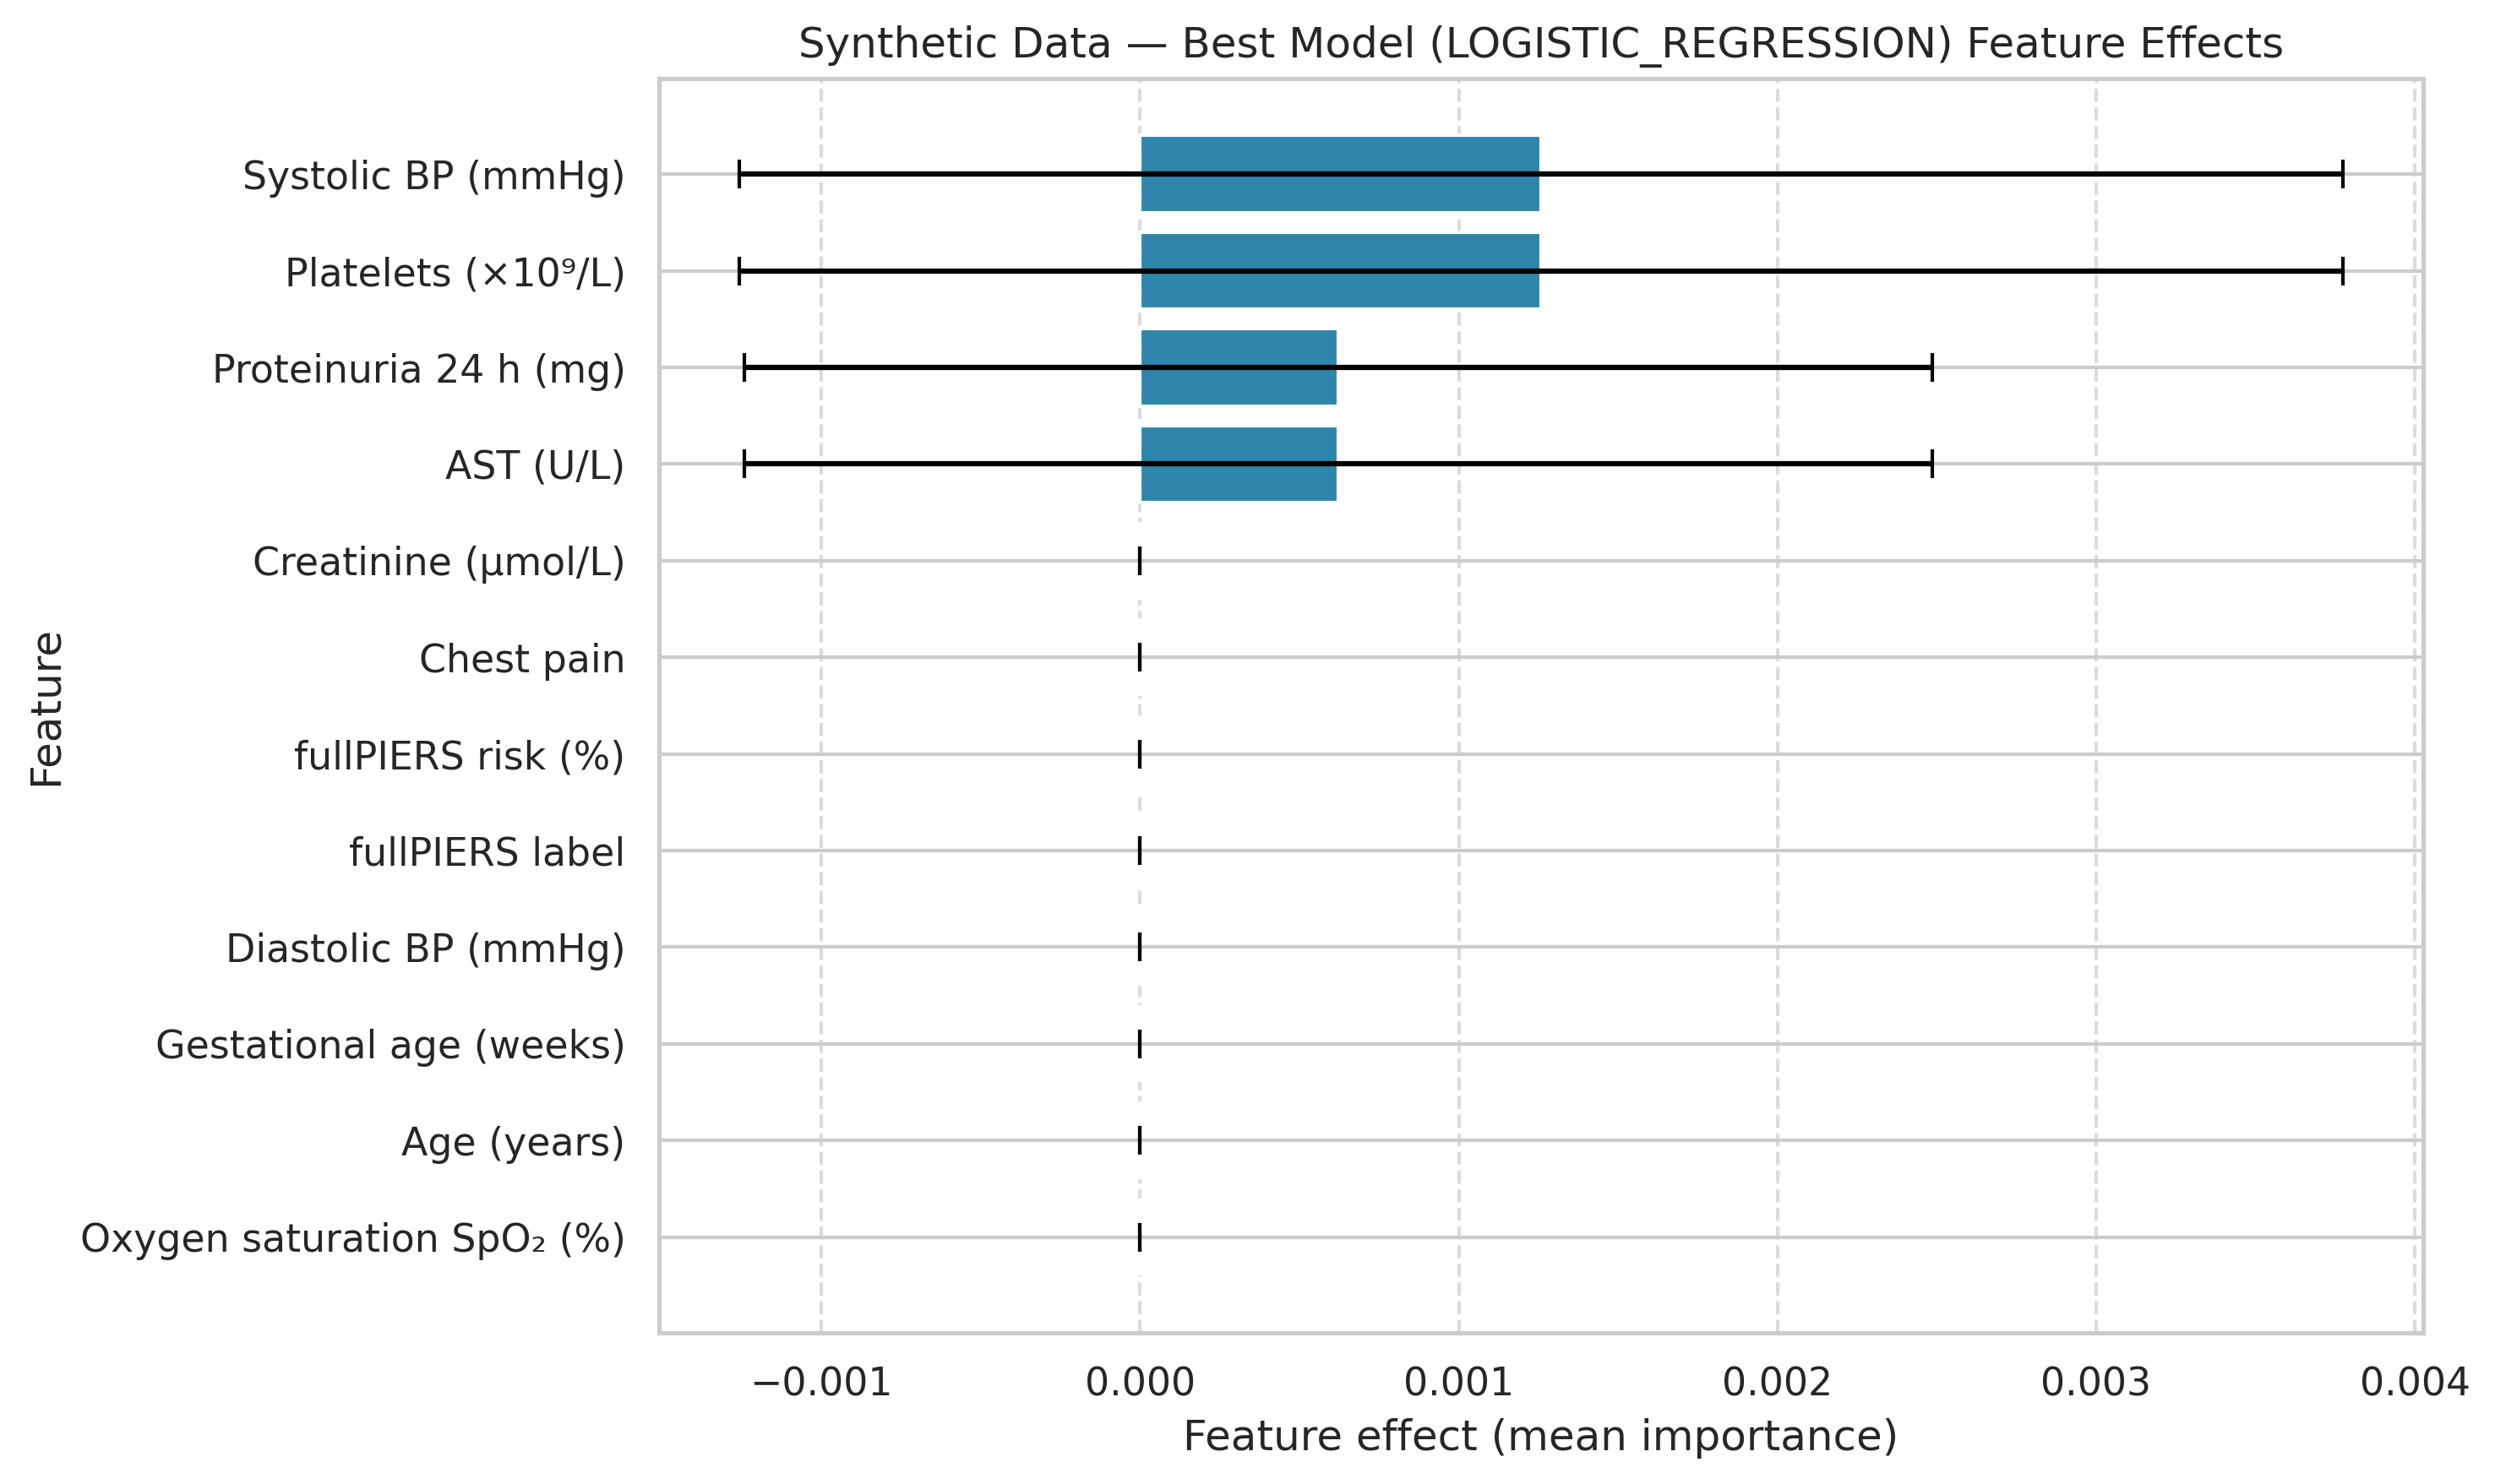
\includegraphics[width=0.48\fulllength]{figures/synthetic_best_model_feature_effects_mean_std.png}}\\
\subfloat[\centering \label{fig:precision-recall-lr-synthetic}]{
  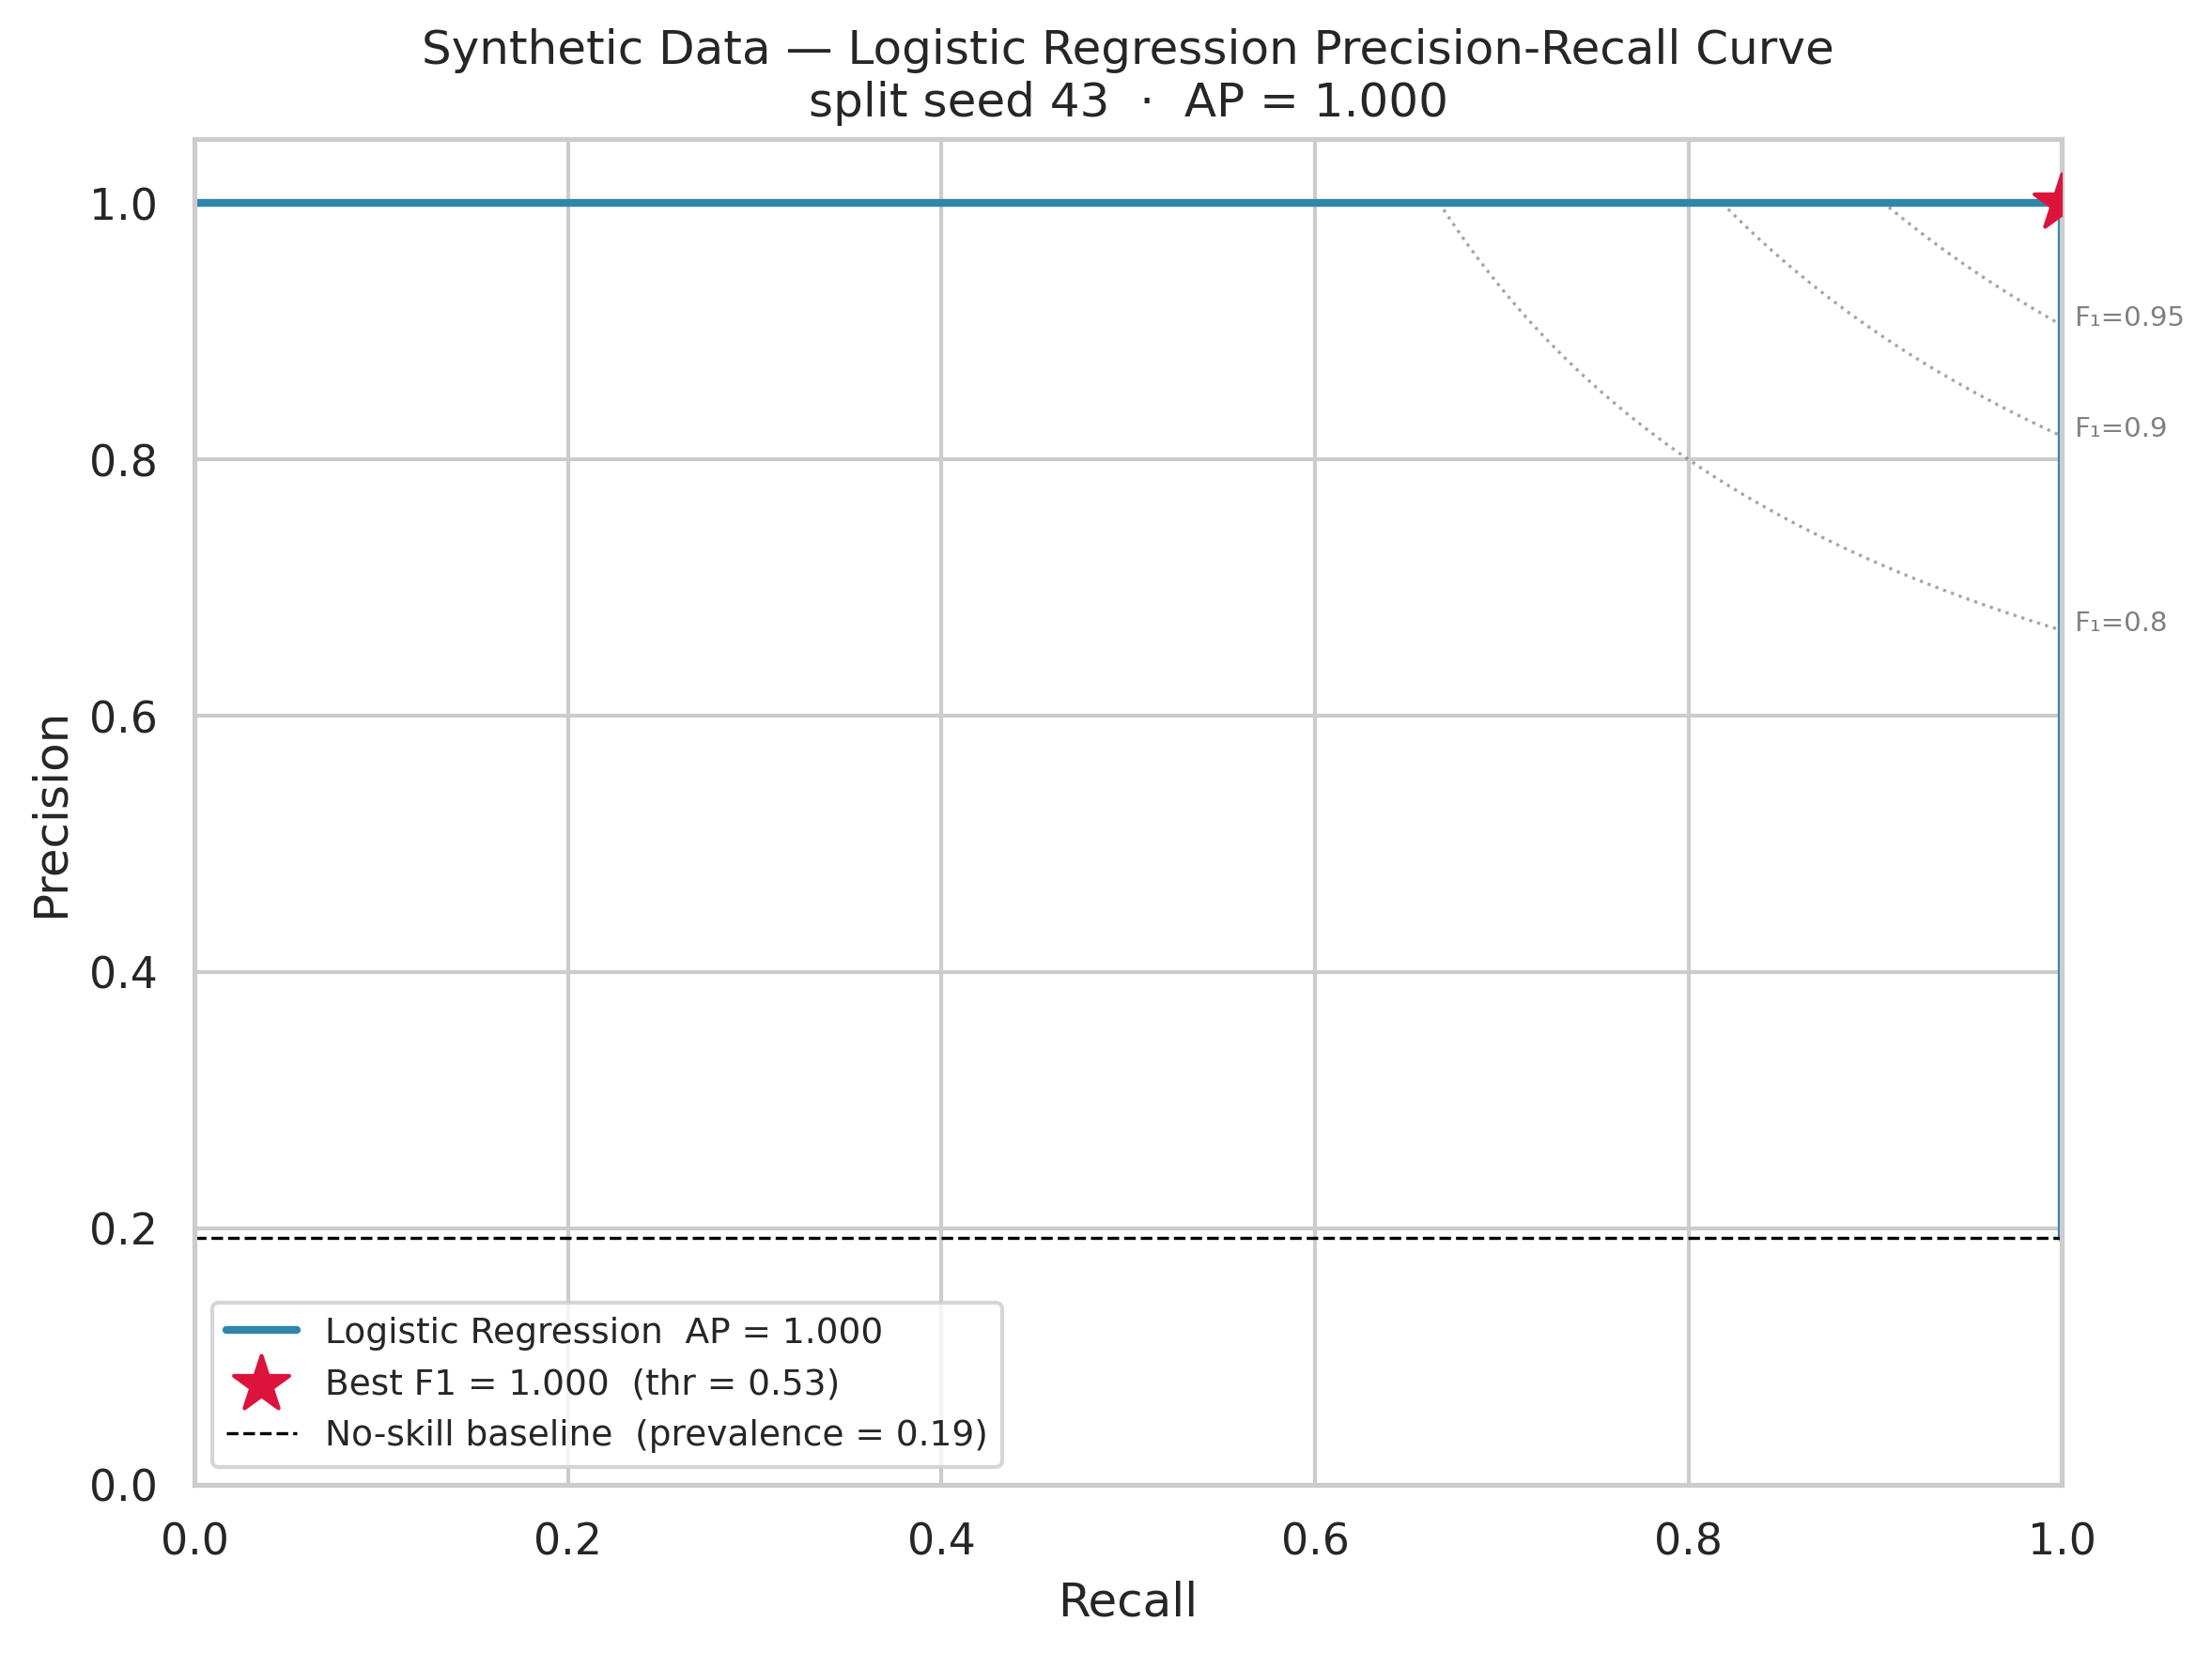
\includegraphics[width=0.48\fulllength]{figures/synthetic_logistic_regression_precision_recall_curve.png}}
\subfloat[\centering \label{fig:f1-score-models-lr-synthetic}]{
  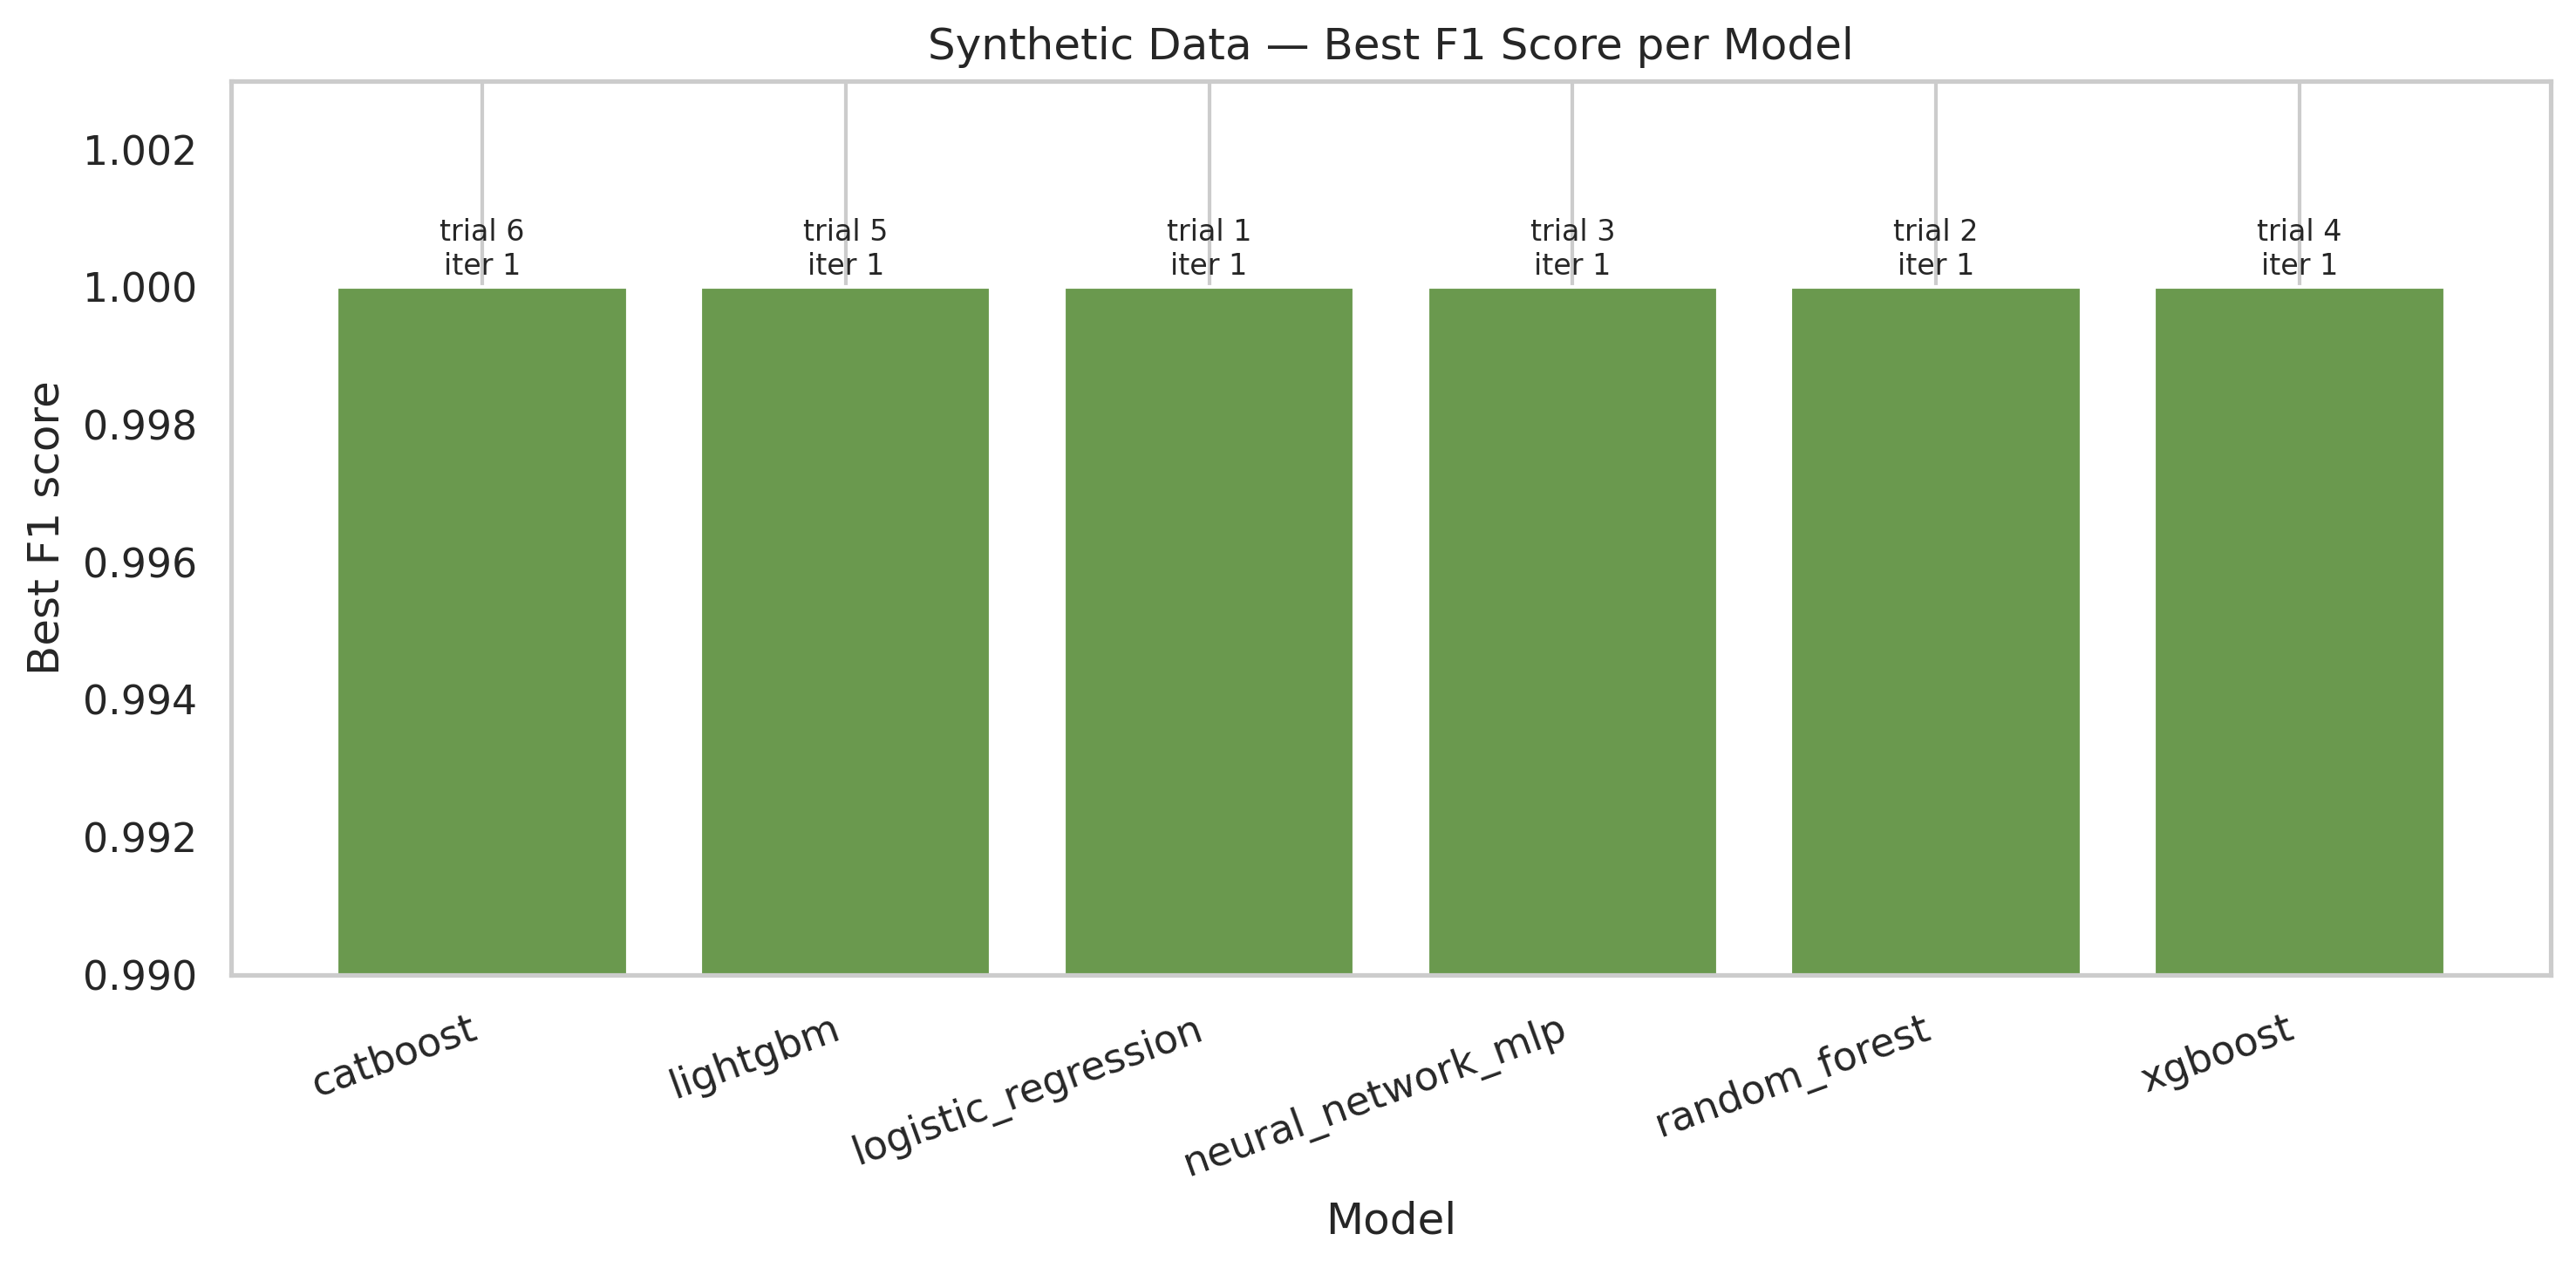
\includegraphics[width=0.48\fulllength]{figures/synthetic_models_best_f1.png}}
\end{adjustwidth}
\caption{{Performance} analysis of the best C-AutoML model (Logistic
  Regression, Trial~1) on the synthetic clinical dataset. (\textbf{a})  Normalized confusion matrix. (\textbf{b})  Mean and standard deviation of feature importance in the
  Logistic Regression prediction on synthetic clinical
  data. (\textbf{c})  Precision--recall curve for the best Logistic Regression
  model on synthetic clinical
  data. (\textbf{d})~F1-score comparison across best model per family on synthetic
  clinical data. % <<AUTHORS: we removed redundant text>>
  \label{fig:combined-model-analysis-synthetic}}
\end{figure}

\vspace{-6pt}

\begin{table}[H]
\caption{C-AutoML performance across trials and iterations on the
  synthetic clinical dataset. Each trial uses a different
  train/validation split and hyperparameter
  configuration.\label{tab:cautoml-synthetic-performance}}
\begin{tabularx}{\linewidth}{LLLCCCCC}
\toprule




\textbf{Trial} & \textbf{Iter} & \textbf{Model} &
\textbf{F1} & \textbf{Acc} & \textbf{Prec} & \textbf{Rec} & \textbf{AUC} \\
\midrule
%\endhead



1  & 1 & \textbf{LR}       & \textbf{1.0000} & \textbf{1.0000} & \textbf{1.0000} & \textbf{1.0000} & \textbf{1.0000} \\
2  & 1 & RF                & 1.0000 & 1.0000 & 1.0000 & 1.0000 & 1.0000 \\
3  & 1 & MLP               & 1.0000 & 1.0000 & 1.0000 & 1.0000 & 1.0000 \\
4  & 1 & XGBoost           & 1.0000 & 1.0000 & 1.0000 & 1.0000 & 1.0000 \\
5  & 1 & LightGBM          & 1.0000 & 1.0000 & 1.0000 & 1.0000 & 1.0000 \\
6  & 1 & CatBoost          & 1.0000 & 1.0000 & 1.0000 & 1.0000 & 1.0000 \\
7  & 2 & LR                & 1.0000 & 1.0000 & 1.0000 & 1.0000 & 1.0000 \\
\bottomrule
\end{tabularx}
\end{table}

\begin{table}[H]\ContinuedFloat
\caption{{\em Cont.}}\label{tab:cautoml-synthetic-performance}

\begin{tabularx}{\linewidth}{LLLCCCCC}
\toprule




\textbf{Trial} & \textbf{Iter} & \textbf{Model} &
\textbf{F1} & \textbf{Acc} & \textbf{Prec} & \textbf{Rec} & \textbf{AUC} \\
\midrule
8  & 2 & RF                & 1.0000 & 1.0000 & 1.0000 & 1.0000 & 1.0000 \\
9  & 2 & MLP               & 1.0000 & 1.0000 & 1.0000 & 1.0000 & 1.0000 \\
10 & 2 & XGBoost           & 1.0000 & 1.0000 & 1.0000 & 1.0000 & 1.0000 \\
11 & 2 & LightGBM          & 1.0000 & 1.0000 & 1.0000 & 1.0000 & 1.0000 \\
12 & 2 & CatBoost          & 1.0000 & 1.0000 & 1.0000 & 1.0000 & 1.0000 \\
13 & 3 & LR                & 1.0000 & 1.0000 & 1.0000 & 1.0000 & 1.0000 \\
14 & 3 & RF                & 1.0000 & 1.0000 & 1.0000 & 1.0000 & 1.0000 \\
15 & 3 & MLP               & 1.0000 & 1.0000 & 1.0000 & 1.0000 & 1.0000 \\
16 & 3 & XGBoost           & 1.0000 & 1.0000 & 1.0000 & 1.0000 & 1.0000 \\
17 & 3 & LightGBM          & 1.0000 & 1.0000 & 1.0000 & 1.0000 & 1.0000 \\
18 & 3 & CatBoost          & 1.0000 & 1.0000 & 1.0000 & 1.0000 & 1.0000 \\
19 & 4 & LR                & 0.9938 & 0.9975 & 0.9877 & 1.0000 & 1.0000 \\
20 & 4 & RF                & 0.9938 & 0.9975 & 0.9877 & 1.0000 & 0.9998 \\
21 & 4 & MLP               & 0.9938 & 0.9975 & 0.9877 & 1.0000 & 1.0000 \\
22 & 4 & XGBoost           & 0.9938 & 0.9975 & 0.9877 & 1.0000 & 1.0000 \\
23 & 4 & LightGBM          & 1.0000 & 1.0000 & 1.0000 & 1.0000 & 1.0000 \\
24 & 4 & CatBoost          & 0.9938 & 0.9975 & 0.9877 & 1.0000 & 1.0000 \\
25 & 5 & LR                & 0.9875 & 0.9950 & 0.9875 & 0.9875 & 1.0000 \\
26 & 5 & RF                & 0.9938 & 0.9975 & 0.9877 & 1.0000 & 1.0000 \\
27 & 5 & MLP               & 0.9938 & 0.9975 & 0.9877 & 1.0000 & 0.9999 \\
28 & 5 & XGBoost           & 0.9938 & 0.9975 & 0.9877 & 1.0000 & 1.0000 \\
29 & 5 & LightGBM          & 1.0000 & 1.0000 & 1.0000 & 1.0000 & 1.0000 \\
30 & 5 & CatBoost          & 0.9938 & 0.9975 & 0.9877 & 1.0000 & 1.0000 \\
\bottomrule

\end{tabularx}
\noindent{\footnotesize{Abbreviations---LR: Logistic Regression;
    RF: Random Forest; MLP: Multi-Layer Perceptron; XGBoost: Extreme
    Gradient Boosting; LightGBM: Light Gradient Boosting Machine;
    CatBoost: Categorical Boosting. \textbf{Bold} row indicates the
    best-performing model overall.}}
\end{table}



\subsection{Artificial Intelligence Explainability}
\label{sec:model-explainability}
\Ac{SHAP}, introduced in \cite{lundberg2017shap}, computes Shapley
values to attribute feature importance for individual predictions. In
this section, we present feature importance results from three
analyses: (i) applying SHAP to the LightGBM model trained on \ac{HGOIA}
data, \mbox{(ii) evaluating} built-in feature importance from
Amazon SageMaker Canvas, and (iii) applying SHAP to the best-performing
model on synthetic clinical data.

% \subsubsection{LightGBM on Isidro Ayora Hospital Dataset}
% \label{sec:lightgbm-isidro-ayor}
\subsubsection*{SHAP Explainability of LightGBM on \ac{HGOIA} Dataset}
\label{sec:lightgbm-isidro-ayor}
Figure~\ref{fig:lightgbm-shap-plots} presents a \ac{SHAP} beeswarm
(Figure~\ref{fig:lightgbm-shap-plots}a) and a
\ac{SHAP} (Figure~\ref{fig:lightgbm-shap-plots}b) waterfall plots that
show the feature importance \ac{w.r.t.} the model output. For
LightGBM, it is noticeable that variable {Age} %<<AUTHOR: removed
% special font>>
was the most influential variable, with higher {values} %<<AUTHOR:
% removed redundant age word>>
producing predominantly positive \ac{SHAP} contributions and thus
increasing the predicted probability of \ac{PE}. \ac{GA} also showed a
strong contribution, with higher values generally associated with
positive model output, whereas {lower} \ac{GA} %<<AUTHOR: replaced
% for the acronym>>
tended to reduce predicted risk. In contrast, BMI {and} weight
{had} %<<AUTHOR: removed special font>>
more moderate effects centered closer to zero, suggesting that they
refined the prediction but contributed less than {Age} %<<AUTHOR:
% uniform writing of the variable age>>
{and} \ac{GA} %<<AUTHOR: replaced with acronym>>
to the final classification. Overall, the explainability analysis
supports that the LightGBM model captured demographically plausible
risk gradients while remaining consistent with the ranking observed in
the performance analysis.
\vspace{-6pt}
\begin{figure}[H]
\begin{adjustwidth}{-\extralength}{0cm}
\centering
\subfloat[\centering \label{fig:lightgbm-beeswarm}]{
  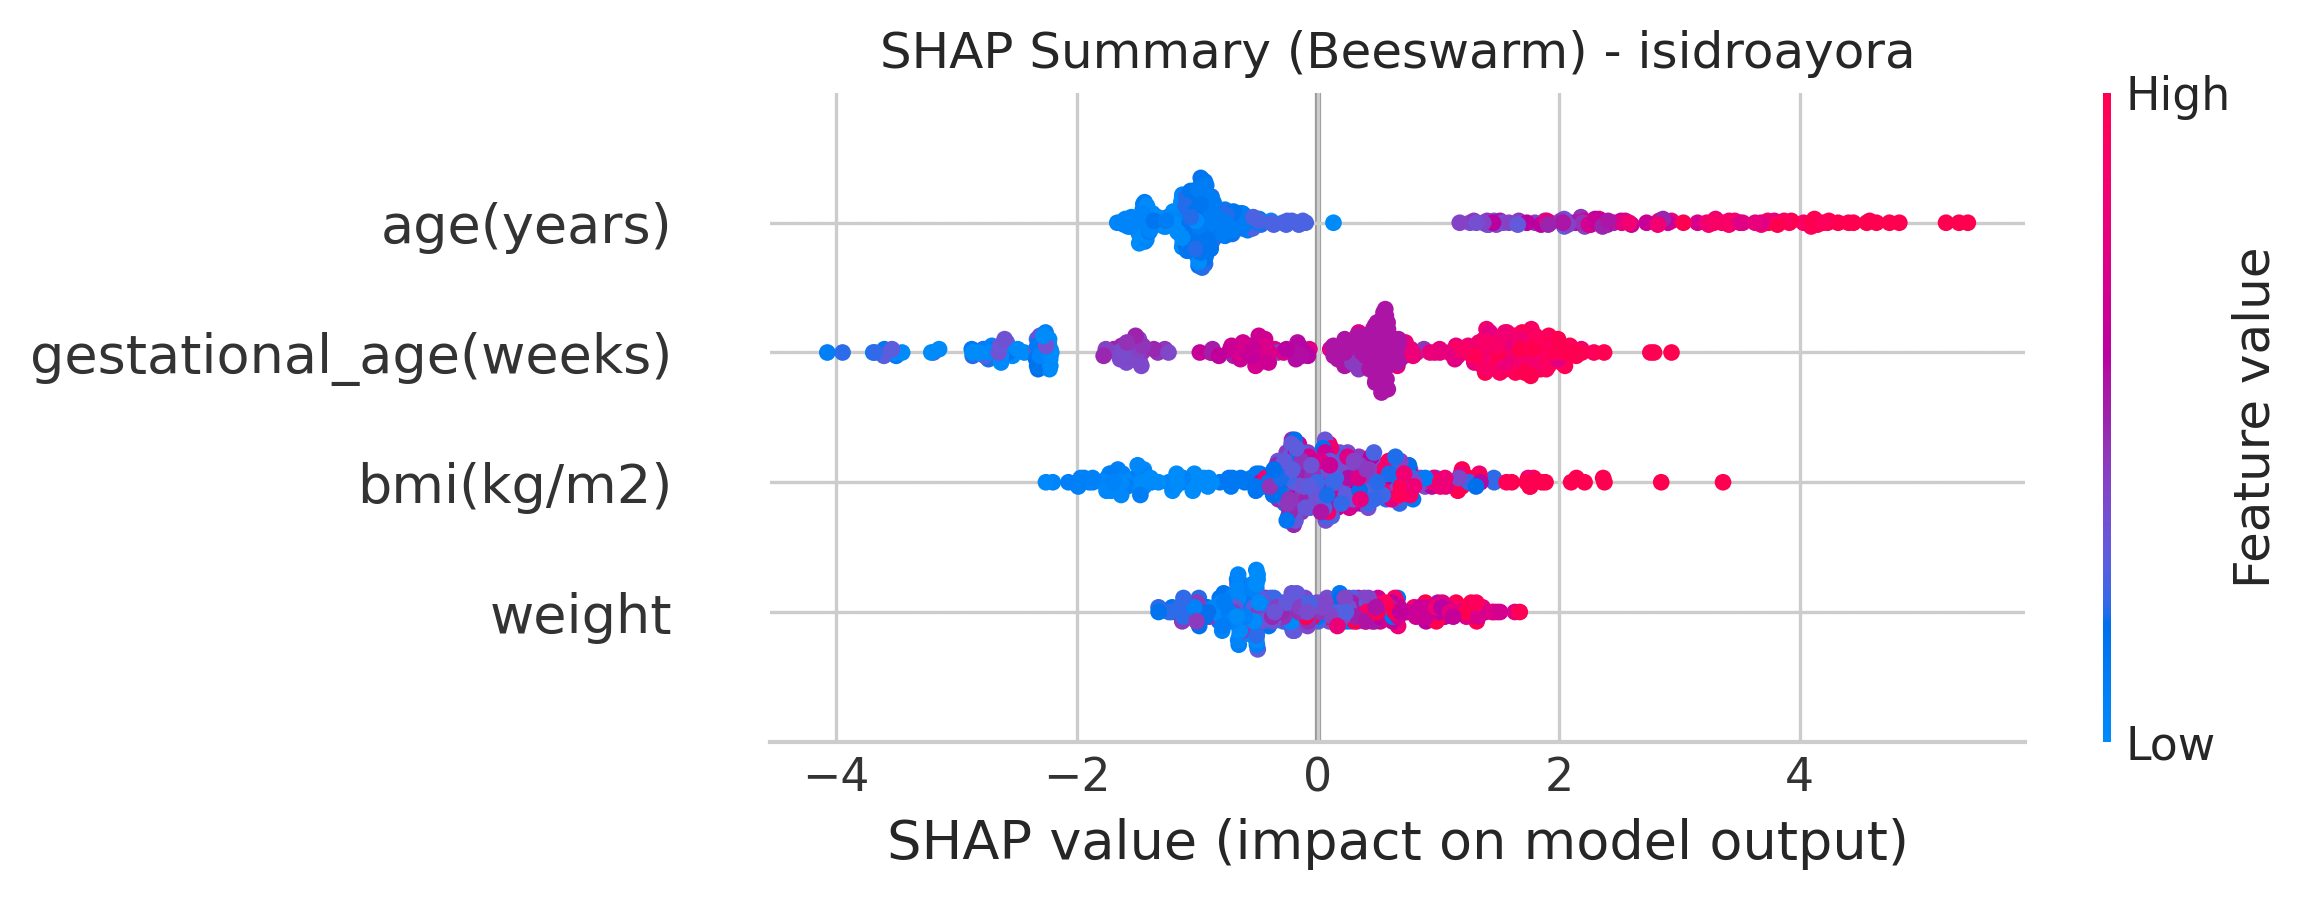
\includegraphics[width=0.89\fulllength]{figures/shap_explainability/isidroayora/shap_summary_beeswarm.png}}\\
\subfloat[\centering \label{fig:lightgbm-waterfall}]{
  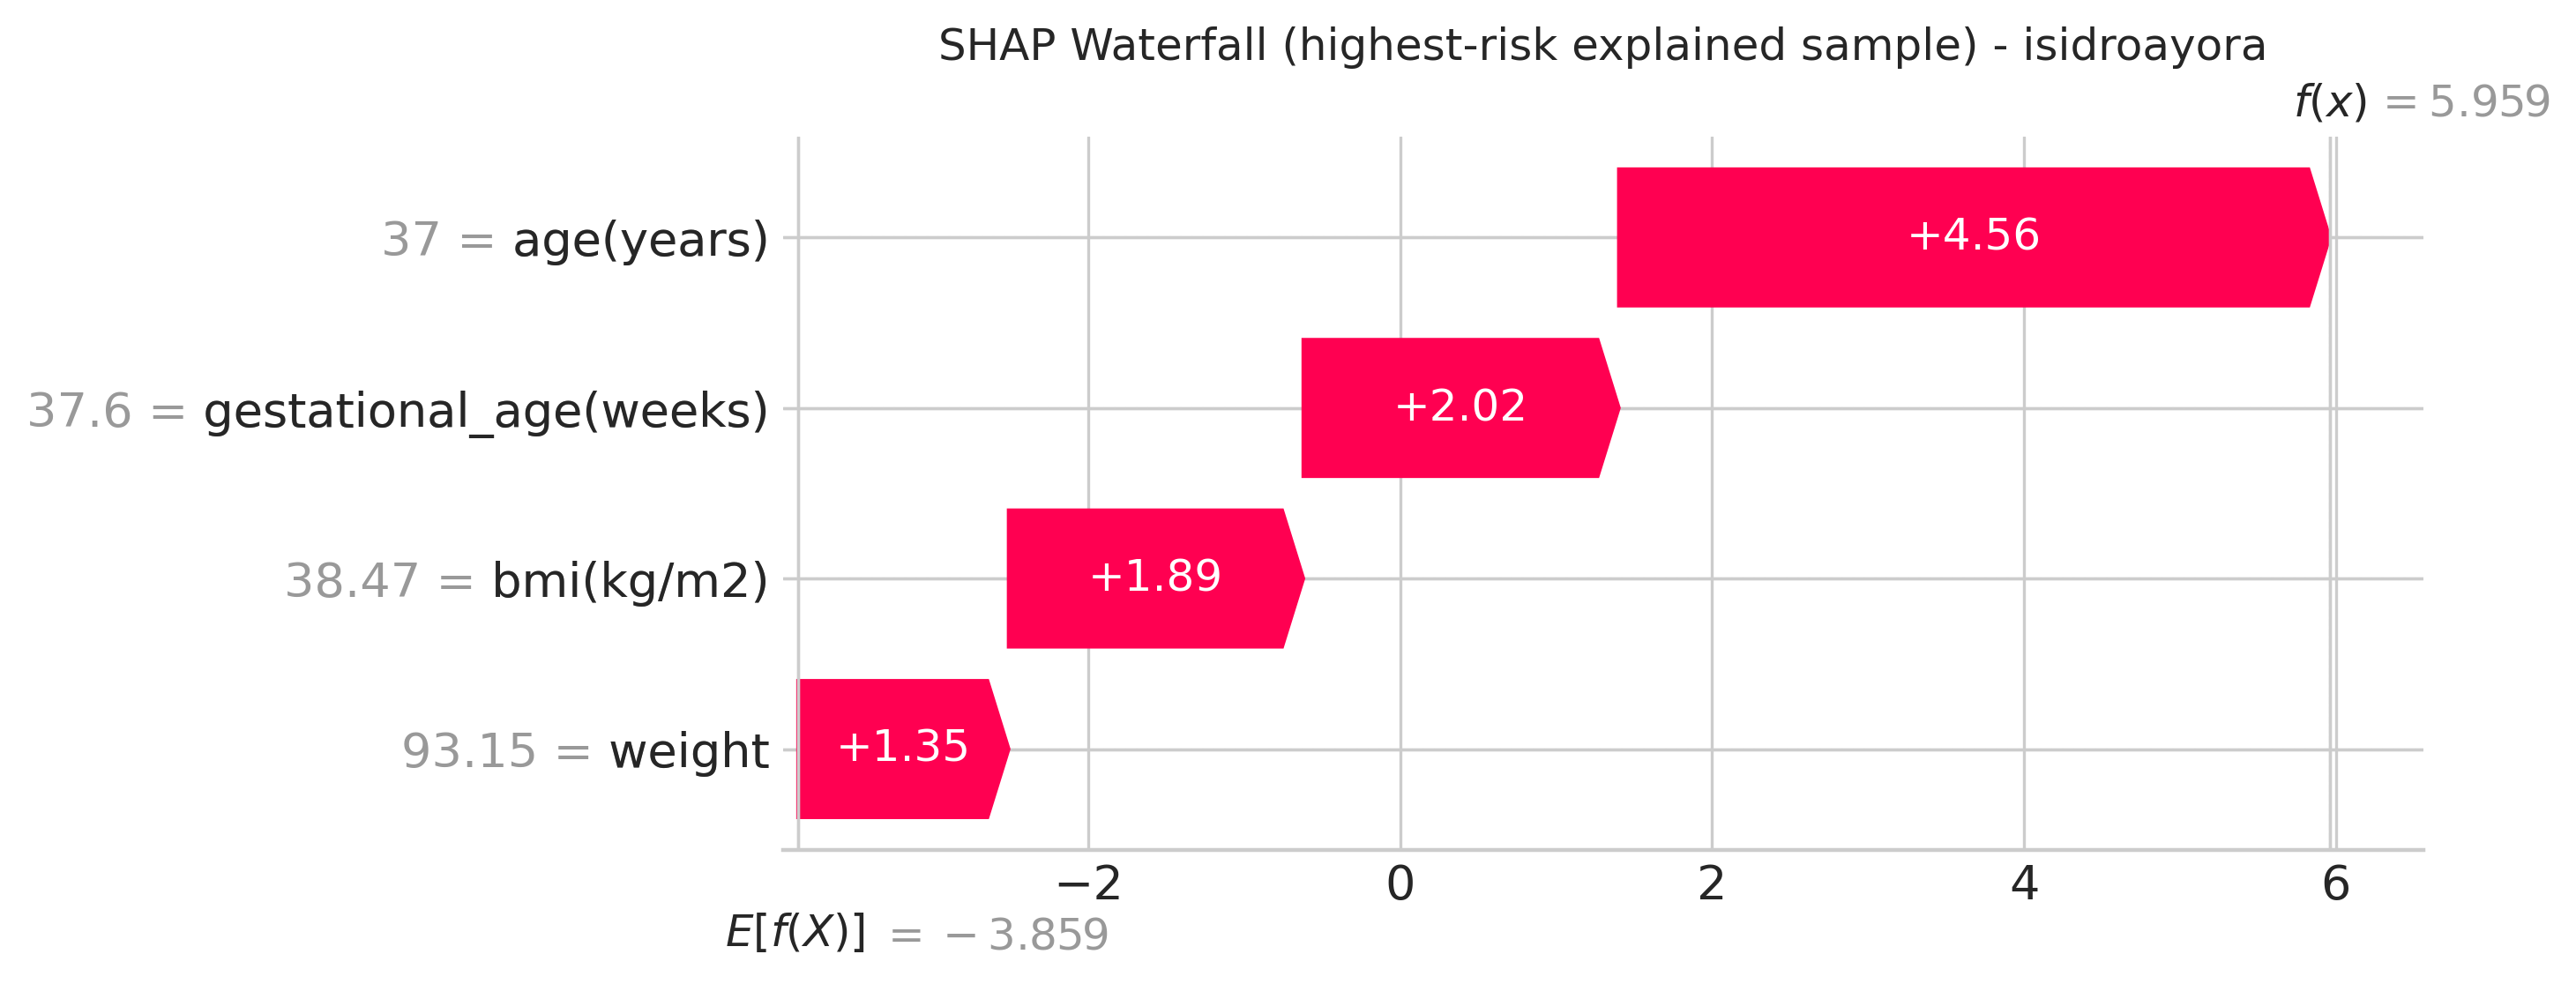
\includegraphics[width=0.89\fulllength]{figures/shap_explainability/isidroayora/shap_waterfall_highest_risk.png}}
\end{adjustwidth}
\caption{SHAP explainability visualizations for the best LightGBM
  model trained on the \ac{HGOIA} dataset. (\textbf{a})
  Global feature importance via beeswarm plot. (\textbf{b}) Local
  instance-level explanation via waterfall plot for the highest-risk
  predicted case. (\textbf{a})  SHAP beeswarm plot summarizing feature importance and impact
  direction. Each point represents a SHAP value for a single feature
  and instance. (\textbf{b}) SHAP waterfall plot for a high-risk instance, illustrating
  how each feature contributes to shifting the model prediction from
  the base value to the final
  output.
  \label{fig:lightgbm-shap-plots}}
\end{figure}

% \subsection{Ensemble Model on Isidro Ayora Dataset (AWS Sage Maker)}
% \label{sec:ensemble-model-xai}
\subsection{SHAP Explainability of the Weighted Ensemble Model on \ac{HGOIA} Dataset}
\label{sec:ensemble-model-xai}

Figure~\ref{fig:canvas-shap-plots} presents the \ac{SHAP} analysis
for the Weighted Ensemble Model trained in Amazon SageMaker
Canvas on the \ac{HGOIA} dataset, including a beeswarm
summary plot (Figure~\ref{fig:canvas-shap-plots}a) and a waterfall plot
for the highest-impact instance (Figure~\ref{fig:canvas-shap-plots}b).

The beeswarm plot reveals that {maternal age} (years) %AUTHOR:
% removed special font>>
is the dominant driver of model output (mean $|\text{SHAP}| = 4.046$),
followed by \ac{GA} {(weeks)} %<<AUTHOR: removed special font>>
(mean $|\text{SHAP}| = 1.847$) {and} \ac{BMI} %<<AUTHOR: removed
% special font>>
(mean $|\text{SHAP}| = 1.335$).  {Maternal weight} %<AUTHOR:
% removed special font>>
contributes with a smaller but still observable effect. This ranking
is consistent with the feature importance observed in the
\ac{C-AutoML} LightGBM model, confirming that {maternal age}
% <<AUTHOR: writing uniformly the variable>>
{and}
% <<AUTHOR: using acronym instead of the word>>
\ac{GA} are the most informative demographic predictors in
this dataset. Notably, approximately 34.9\% of feature contributions
are positive and 65.1\% are negative across all feature--instance
pairs, indicating that feature effects are bidirectional and
patient-specific rather than uniformly monotonic.  Higher values of
{maternal age} %<<AUTHOR: uniform maternal age>>
(shown in red) are associated with predominantly positive
\ac{SHAP} contributions, pushing predictions toward \ac{PE}, while
lower values (blue) tend to reduce predicted risk.

\vspace{-6pt}
\begin{figure}[H]
\begin{adjustwidth}{-\extralength}{0cm}
\centering
\subfloat[\centering \label{fig:canvas-beeswarm}]{
  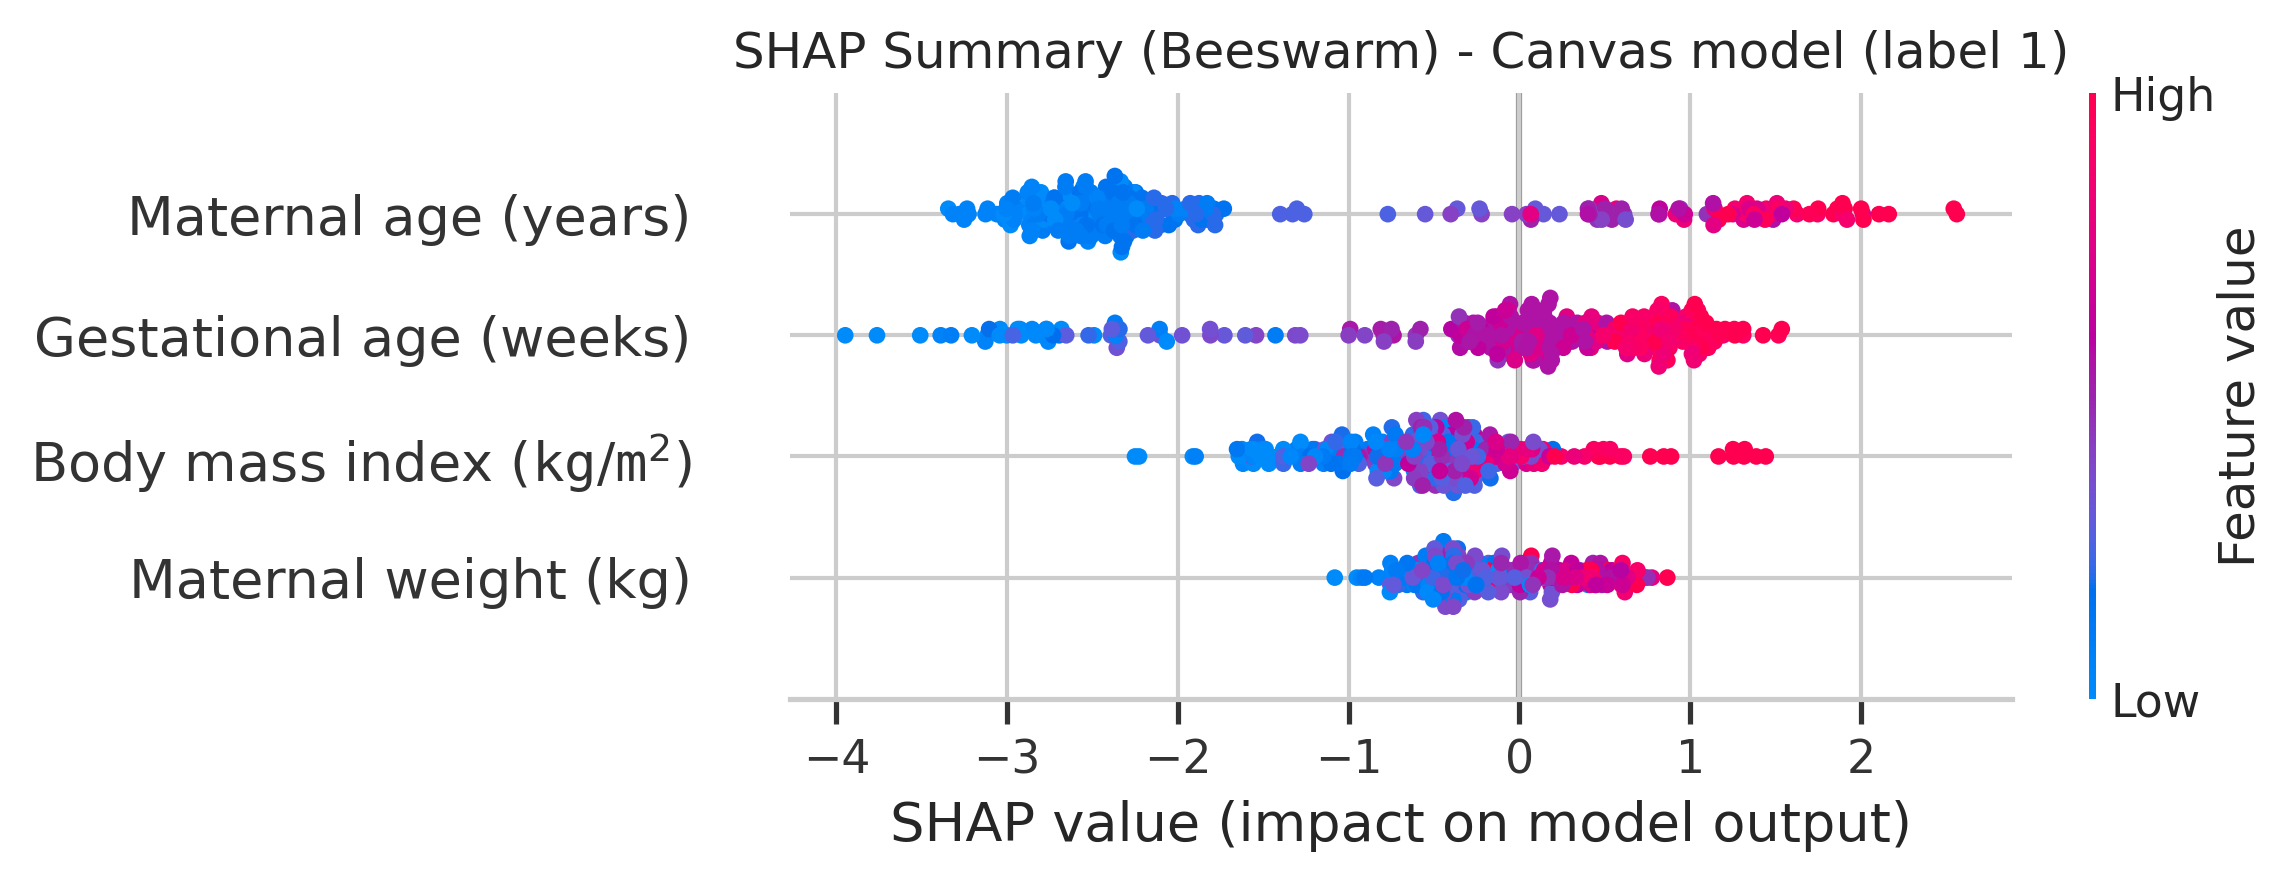
\includegraphics[width=0.95\fulllength]{figures/shap_explainability/canvas_sagemaker_model/canvas_shap_beeswarm_summary_label1.png}}\\
\subfloat[\centering \label{fig:canvas-waterfall}]{
  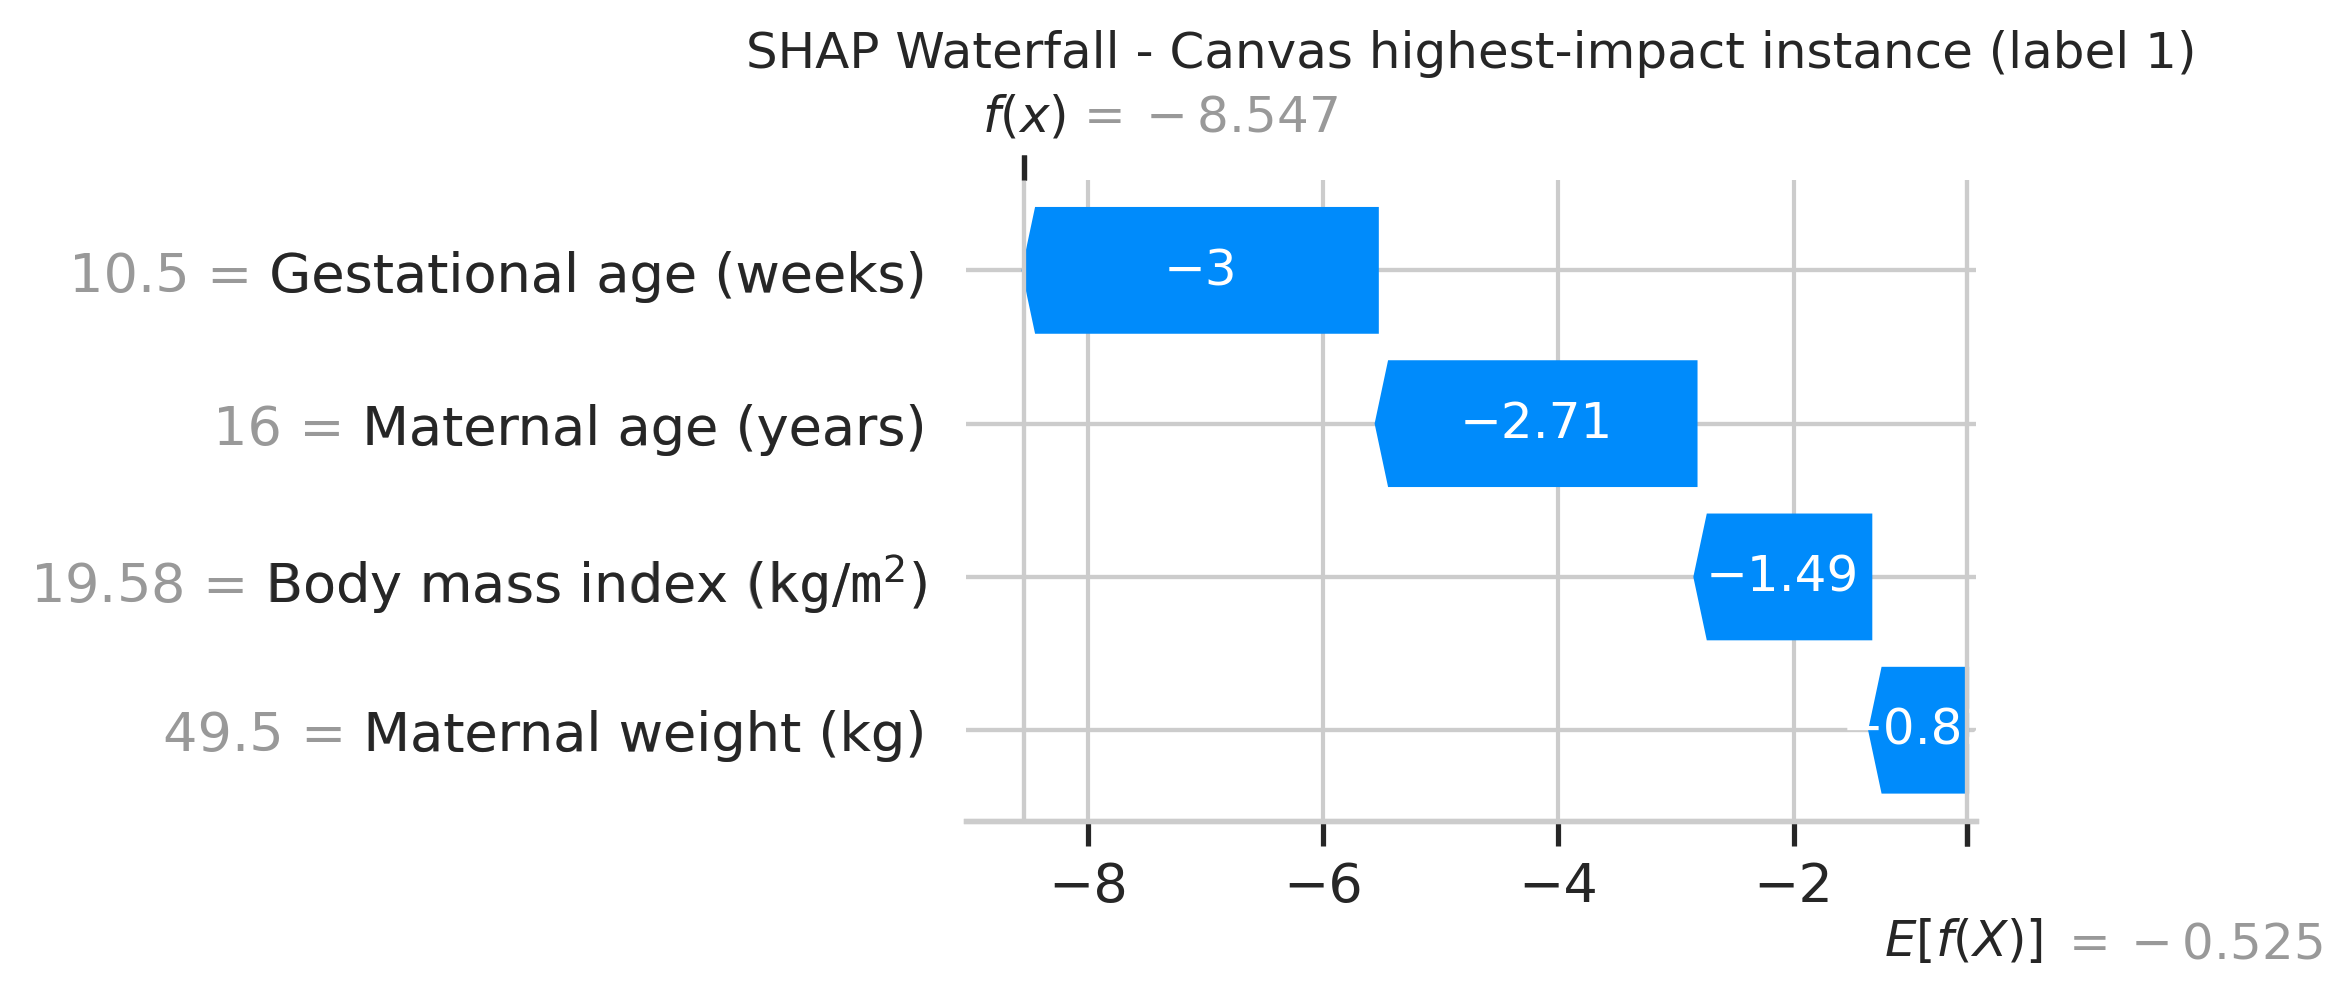
\includegraphics[width=0.95\fulllength]{figures/shap_explainability/canvas_sagemaker_model/canvas_shap_waterfall_high_impact_label1.png}}
\end{adjustwidth}
\caption{\ac{SHAP} explainability visualizations for the Amazon SageMaker
  Canvas Weighted Ensemble Model on the \ac{HGOIA} dataset.
  (\textbf{a}) Global feature importance via beeswarm plot; maternal
  age is the dominant contributor (mean $|\text{SHAP}|=4.046$).
  (\textbf{b}) Local instance-level explanation via waterfall plot for
  the highest-impact predicted case.  (\textbf{a}) \ac{SHAP} beeswarm summary plot for the Weighted Ensemble
  Model. Each point represents a \ac{SHAP} value for a single feature
  and instance; color encodes feature
  value.  (\textbf{b})  \ac{SHAP} waterfall plot for the highest-impact instance
  (index 36), showing how each feature shifts the prediction from the
  base value $E{[f(X)]}=-0.525$ to the final output
  $f(\mathbf{x})=-8.547$.
  \label{fig:canvas-shap-plots}}
\end{figure}

\textls[-15]{The waterfall plot for the highest-impact instance (index 36,
$f(\mathbf{x}) = -8.547$, $E[f(X)] = -0.525$) illustrates a case
where all four features act in the same direction. \ac{GA} {at}
% <<AUTHOR: use of acronym>>
10.5 weeks contributes $-3.002$ \ac{SHAP} units, {maternal
  age} %<<AUTHOR: removed special font>>
at 16 years contributes $-2.710$, \ac{BMI} {at} %<<AUTHOR: use of
                                %acronym and removal of special font
                                %for BMI>>
19.58~kg/m$^2$ contributes $-1.486$, and {maternal weight}
% <<AUTHOR: removed special font for maternal weight>>
at 49.5~kg contributes $-0.8$, cumulatively shifting the prediction
well below the base value. This pattern is clinically coherent: a very
young patient at {early} %<<AUTHOR: use of gestational age
% acronym>>
\ac{GA} with low \ac{BMI} and weight presents a low-risk demographic
profile, and the model correctly assigns a strong negative
prediction. Taken together, the global and local \ac{SHAP} analyses
confirm that the {Weighted Ensemble} %<<AUTHOR: removed the special
% font>>
Model captures clinically plausible risk gradients from demographic
variables alone, and that its decision structure is interpretable and
consistent with the known epidemiology \mbox{of \ac{PE}.}}



% \subsection{Logistic Regression on Synthetic Data}
% \label{sec:lorg-regr-synth-xai}
\subsubsection*{SHAP Explainability of Logistic Regression on Synthetic Clinical Data}
\label{sec:lr-synthetic-xai}

Figure~\ref{fig:synthetic-shap-plots} presents the \ac{SHAP} analysis
for the \ac{LR} model trained on the synthetic clinical dataset,
including a beeswarm summary plot
(Figure~\ref{fig:synthetic-shap-plots}a) and a waterfall plot for the
highest-risk instance (Figure~\ref{fig:synthetic-shap-plots}b).

\vspace{-6pt}
% Sonet 4.6 Adaptive
\begin{figure}[H]
\subfloat[\centering \label{fig:synthetic-beeswarm}]{
  
\includegraphics[width=0.98\fulllength, height=.35\textheight, keepaspectratio]{figures/shap_explainability/synthetic_fullpiers/shap_summary_beeswarm.png}}\\
\subfloat[\centering  \label{fig:synthetic-waterfall}]{
  
\includegraphics[width=0.98\fulllength, height=.35\textheight, keepaspectratio]{figures/shap_explainability/synthetic_fullpiers/shap_waterfall_highest_risk.png}}
\caption{\ac{SHAP} explainability visualizations for the best \ac{LR}
  model trained on the synthetic clinical dataset. (\textbf{a})
  Global feature importance via beeswarm plot; \ac{DBP} and \ac{SBP}
  are the dominant contributors. (\textbf{b}) Local instance-level
  explanation via waterfall plot for the highest-risk predicted case,
  dominated by \ac{AST}, proteinuria, and blood pressure. (\textbf{a}) \ac{SHAP} beeswarm summary for the \ac{LR} model on
  synthetic clinical data. Each point represents a \ac{SHAP} value
  for a single feature and instance; color encodes feature
  value.  (\textbf{b}) \ac{SHAP} waterfall plot for the highest-risk instance
  ($f(\mathbf{x})=8.976$, $E{[f(X)]}=-0.604$), showing cumulative
  feature contributions from the base value to the final
  output.
  \label{fig:synthetic-shap-plots}}
\end{figure}


The beeswarm plot reveals a feature-importance structure that is
highly consistent with the rule-based and prognostic variables used to
construct the data. \ac{DBP} and \ac{SBP} appear among the strongest
positive contributors, with higher values (red) shifting the
prediction toward \ac{PE}. \texttt{Proteinuria\_24h\_mg},
\ac{AST}, creatinine, and the FullPIERS risk percentage also display
predominantly positive \ac{SHAP} values at higher feature levels,
indicating that the model assigns greater risk when these markers of
renal, hepatic, and overall maternal severity increase. In contrast,
higher platelet counts, $\text{SpO}_2$, {and} \ac{GA} %<<AUTHOR:
% using acronym for gestational age>>
tend to move predictions toward lower risk, reflected by negative
\ac{SHAP} contributions at higher values. Age shows a smaller but
still coherent contribution, while chest pain has a limited overall
effect due to its low prevalence in the dataset.

The waterfall plot for the highest-risk instance ($f(\mathbf{x}) =
8.976$, $E{[f(X)]} = -0.604$) confirms this interpretation at the
local level. \ac{AST} (=4.518~U/L) and
\texttt{Proteinuria\_24h\_mg} (=3.275~mg) each contribute
+1.56 \ac{SHAP} units, followed by low $\text{SpO}_2$ (=$-$3.192)~({feature values shown in the waterfall plot
  correspond to the scaled representations used internally by the
  \ac{LR} pipeline in \ac{C-AutoML}}) at $+1.19$, \ac{DBP} (=2.835) at +1.16, and \ac{SBP}
(=2.519) at +1.02. The FullPIERS risk percentage and the
FullPIERS diagnostic label add a further $+0.99$ and $+0.98$
respectively, while chest pain makes a small negative contribution of
$-0.05$. The additive accumulation of hemodynamic, renal, and hepatic
abnormalities drives the final output far above the base value,
confirming that the \ac{LR} model identifies high-risk cases through a
clinically coherent combination of severity indicators. Taken
together, the global and local \ac{SHAP} analyses demonstrate that
the model learned a decision structure dominated by classical
\ac{PE} risk markers and is fully consistent with the
rule-based labels used during synthetic data generation.

%\newpage
\section{Discussion}
\label{sec:discussion}

In this study, we explored different models and approaches to train a
robust model for the prediction of \ac{PE}. To this end, we
used the data provided by the Isidro Ayora Gynecology and Obstetrics
Hospital (\ac{HGOIA}). However, the digital records are predominantly
demographic. For this reason, we generated a synthetic dataset using
variables commonly found in \ac{PIERS}.

For the \ac{HGOIA} dataset, we trained models with our
proposed methodology named \ac{C-AutoML}, where we compared the
performance of up to six different Machine Learning models. Our approach
aims to improve performance by exposing the models to different
training and validation splits during each trial and also searches
for the best hyperparameter configuration. The best model found corresponded
to LightGBM. In parallel, we trained additional
Machine Learning models using Amazon SageMaker Canvas, which produced as
best model a Weighted Ensemble Model. Finally, for the
clinical synthetic dataset, \ac{LR}, among other models, achieved
ideal performance.

Our results show that the Weighted Ensemble Model achieved
the best performance for the \ac{HGOIA} dataset because it
has the highest recall ($\mathrm{Recall}=0.844$), compared to that of
LightGBM ($\mathrm{Recall}=0.768$). This is important
because recall (sensitivity) measures the proportion of women with
\ac{PE} that the model correctly identified. For a medical setting, it is necessary that the model has a
high recall because that lowers the false negatives. As a matter of
fact, the Weighted Ensemble Model loses one in six cases of
\ac{PE}. On the other hand, the LightGBM trained with
our proposed \ac{C-AutoML} approach has a higher precision
($\mathrm{Precision}=0.837$) compared to the Weighted Ensemble
  Model ($\mathrm{Precision}=0.770$). This result is advantageous
because higher precision implies fewer false alarms. Consequently, it is
recommended to combine both of these models for prediction at the
health facility.

For the synthetic dataset, all six evaluated model
  families achieve near-perfect performance ($\mathrm{F1}\geq 0.988$),
  with \ac{LR}, \ac{RF}, \ac{MLP}, XGBoost, LightGBM, and CatBoost all
  reaching $\mathrm{F1}=1.000$ in the first three iterations. This
  high performance is a design consequence: diagnostic labels are
  assigned by a deterministic rule
  (Equation~\eqref{eq:preeclampsia-msp-rule}) applied to the same
  features used as model inputs, creating linearly separable class
  boundaries. The synthetic track serves as a controlled feasibility
  experiment that confirms the \ac{C-AutoML} pipeline operates
  correctly on data with a known ground truth to predict \ac{PE}; it
  does not constitute a clinical performance claim. Notably, the
  inclusion {of} $\text{SpO}_2$, % <<AUTHOR: uniform as in
  % equation>>
  chest pain, platelet count, creatinine, and \ac{AST} in the
  synthetic track is grounded in the published FullPIERS equation
  (Equation~\eqref{eq:fullpiers-logit}), which uses precisely these
  variables as predictors~\cite{fullpiers_2011}. However, it must be
  noticed that the purpose of ~\eqref{eq:fullpiers-logit} is to
  predict adverse outcomes of \ac{PE}, which differs from our main
  purpose.
%% [OLD R1]: For
%%   the synthetic dataset, our results show an ideal performance due to
%%   the controlled synthetic data generation. Nevertheless, the results
%%   identify \ac{LR} as a suitable model for a \ac{PIERS} application.

  The interpretability analysis shows the feature importance of the
  variables of each dataset for prediction. For the \ac{HGOIA}
  dataset, the most important features are: patient's age, \ac{GA},
  {and} %<<AUTHOR: use of gestational age acronym>>
  \ac{BMI}. On the other hand, for the generated synthetic data,
  systolic blood pressure, platelet count and 24 h proteinuria lead
  the impact on model's\mbox{ prediction.}

% R2 BEGIN: comparison with similar-framework studies
% \textbf{Comparison with similar frameworks.}
  
\subsection{Comparison with Similar Frameworks}
\label{sec:comp-with-similar-frameworks}

{Table}~\ref{tab:ml_pe_comparison} %<<AUTHOR: changed to subsection
% to avoid the use of bold font>>
situates our results among studies that employ comparable model
families and predictor types.  Despite using only four demographic
variables, our best models achieve discrimination metrics
(AUC~0.944--0.956, F1~0.802--0.805) that fall within the range
reported for tree-based ensembles operating on richer predictor
sets~\cite{LI2021102,liu_pregnancy_trajectories_2022,zeng_preeclampsia_ml_china_2024,advancing_ml_preeclampsia_2025}.
Direct numerical ranking across studies is discouraged by the
substantial heterogeneity in populations, predictor availability, and
outcome definitions documented in recent systematic
\mbox{reviews~\cite{Darsareh2024,Rahman2023,jmijr_ml_pe_review_2026}.} Consequently,
the comparison in Table~\ref{tab:ml_pe_comparison} is intended to
contextualize rather than rank performance.

\begin{table}[H]
  \small
  \centering
  \caption{Comparison of selected Machine Learning
    studies for preeclampsia prediction using tabular demographic
    and clinical data.\label{tab:ml_pe_comparison}}
  \begin{adjustwidth}{-\extralength}{0cm}
  \begin{tabularx}{\fulllength}{lLLL} %p{3.8cm}p{3.2cm}
    \toprule
    \textbf{Study} & \textbf{Population/Data Source} & \textbf{Main Predictors} & \textbf{Best Model and Performance} \\
    \midrule
    Li et al.\ (2021)~\cite{LI2021102} &
    3759 pregnancies, EHR from a tertiary hospital in China &
    38 routine clinical parameters at early second trimester (incl.\ fasting plasma glucose, mean blood pressure, BMI) &
    XGBoost; AUC~0.955, accuracy~0.920 (F1~0.571) \\
    \addlinespace
    Liu et al.\ (2022)~\cite{liu_pregnancy_trajectories_2022} &
    EMR-based cohort with longitudinal pregnancy data &
    Repeated measures of vital signs and laboratory values across gestation &
    Ensemble ML on trajectories; AUC ${>}\,0.90$ for late-gestation PE \\
    \addlinespace
    Zeng et al.\ (2024)~\cite{zeng_preeclampsia_ml_china_2024} &
    Population-based Chinese cohort &
    Maternal characteristics and first-trimester biomarkers (e.g., PLGF, PAPP-A) &
    Ensemble ML; AUC~0.80--0.86 \\
    \addlinespace
    Advancing ML tools (2025)~\cite{advancing_ml_preeclampsia_2025} &
    Hospital-based cohort &
    Demographic and clinical variables (incl.\ blood pressure and laboratory markers) &
    CatBoost, LightGBM, XGBoost, RF; accuracy~0.90, AUC ${>}\,0.90$ \\
    \addlinespace
    \textbf{This study (HGOIA)} &
    \textbf{4165 pregnancies, public hospital in Ecuador} &
    \textbf{Four demographic variables (age, gestational age, BMI, weight)} &
    \textbf{LightGBM (C-AutoML): F1~0.802, AUC~0.944; Weighted Ensemble (Canvas): F1~0.805, AUC~0.956} \\
    \bottomrule
  \end{tabularx}
  \end{adjustwidth}
\end{table}
% R2 END

% R1.3 BEGIN: Limitations paragraph added per Reviewer 1 (Discussion: "Expand
% discussion on use of demographic-only dataset, single-center study design,
% and synthetic data limitations") and Reviewer 2 (Discussion: "State
% explicitly the strengths and limitations of the study").
% The record-level split statistics are documented in code/patient_split_report.csv.
% \textbf{Limitations.}

\subsection{Limitations}
\label{sec:limitations}

{Several} %<<AUTHOR: we use subsection instead of the bold font>>
limitations of this study should be considered.  First, the \ac{HGOIA}
dataset contains only demographic variables (age, weight, \ac{BMI},
and \ac{GA} {in} %<<AUTHOR: using acronym for gestational
% age>>
weeks); the absence of laboratory and clinical
measurements restricts predictive granularity and precludes direct comparison
with clinically richer models.
Second, this is a single-center, retrospective study conducted at a single
public hospital; generalizability to other institutions or geographic contexts
remains to be evaluated.
Third, the train--validation split in \ac{C-AutoML} was performed at the record
level rather than the patient level. Given that the source dataset contains on
average 1.81 records per patient (range 1--13), the reported
validation metrics may be modestly optimistic and patient-level
cross-validation is recommended for future work.
Finally, the synthetic dataset, while useful for assessing the
feasibility of our proposed framework, does not constitute external clinical validation.

% \textbf{Limitations.}
% Several limitations of this study should be considered.
% First, the \ac{HGOIA} dataset contains only demographic variables (age, weight,
% \ac{BMI}, and gestational age in weeks); the absence of laboratory and clinical
% measurements restricts predictive granularity and precludes direct comparison
% with clinically richer models.
% Second, this is a single-center, retrospective study conducted at a single
% public hospital; generalizability to other institutions or geographic contexts
% remains to be evaluated.
% Third, the train--validation split in \ac{C-AutoML} was performed at the record
% level rather than the patient level: because the source dataset contains on
% average 1.81 records per patient (range 1--13), approximately 61\% of
% validation records originate from patients also present in the training set;
% as the demographic features are correlated within a patient, the reported
% validation metrics may be modestly optimistic and patient-level
% cross-validation is recommended for future work.
% Finally, the synthetic dataset, while useful for assessing the feasibility of
% \ac{PIERS}-style prediction, does not constitute external clinical validation;
% the ideal performance of \ac{LR} on that dataset reflects the mathematical
% separability imposed by the parametric generation distributions, not
% necessarily clinical utility in a real population.
% R1.3 END

% R2 BEGIN: chronic HTN selection + PE sub-categories
Regarding patient selection, the positive class was constructed
exclusively from records matching ICD-10 codes O11, O13, O14, O15, and O16,
as documented in Table~\ref{tab:cie10-icd10-mapping}. Patients with pre-existing
chronic hypertension without superimposed preeclampsia (ICD-10 O10) were absent
from both classes by design: the negative class consists solely of normal
pregnancy supervision records (ICD-10 Z340, Z348, Z349). However, cases of
superimposed preeclampsia on chronic hypertension (ICD-10 O11) are present in
the positive class and represent a subgroup with a physiopathological background
that partially differs from de~novo gestational preeclampsia; separate analysis
of O11 cases is recommended as future work. Additionally, stratified analysis by
\ac{PE} sub-category (early vs.\ late onset; moderate vs.\ severe) was not
feasible with the available data, which records binary \ac{PE} diagnosis without
severity grade or \ac{GA} {at} %<<AUTHOR: use of gestational age
% acronym>>
onset; subgroup analysis constitutes a direction for future research.

Notwithstanding these limitations, this study benefits from
a real-world hospital dataset, a reproducible C-AutoML pipeline with full
artifact tracking via MLflow, SHAP-based interpretability, and benchmarking
against a commercial AutoML platform (Amazon SageMaker Canvas).
% R2 END

\section{Conclusions}
\label{sec:conclusion}
This study explored the performance of different Machine Learning
models towards the prediction of \ac{PE} in the population of
women at the Isidro Ayora Gynecology and Obstetrics {Hospital}
(\ac{HGOIA}). %<<AUTHOR: added parenthesis to the acronym since the
              %name of the hospital was introduced on purpose to aid
              %skim readers>>
Amazon SageMaker Canvas was pivotal in
assessing the predictive power of each of the features from the
provided dataset. Selecting features with high predictive power
prevented our models from overfitting, improving training. To the best of our
knowledge, this is the first study combining patient datasets from
Ecuador with Machine Learning. Our results show that a combination of
our proposed methodology with the trained model from Canvas can lead
to effective predictions at the health facility.

Our proposed training methodology improved the hyperparameter settings
of different models targeting the \ac{F1} metric, which balances
precision and recall, where the latter is of most importance for a
medical application because it measures the proportion of true
\ac{PE} cases correctly identified by the model, whereas the
former accounts for the cost of false alarms. We prioritize recall
because it emphasizes minimizing missed diagnoses.

LightGBM achieved the best performance \ac{w.r.t.} the
\ac{F1} metric using our proposed \ac{C-AutoML} workflow, with
$\mathrm{F1}=0.802$, $\mathrm{Recall}=0.768$, and
$\mathrm{Precision}=0.837$. This means that 77\% of true \ac{PE}
cases were correctly detected by the model. Consequently, this model
misses one out of four true \ac{PE} cases. On the other hand, the
Weighted Ensemble Model trained in Amazon SageMaker Canvas achieved an
$\mathrm{F1}=0.805$, $\mathrm{Precision}=0.770$, and
$\mathrm{Recall}=0.844$. Therefore, 84\% of true \ac{PE} cases
were correctly detected by the ensemble model and misses 1 out of 6
true \ac{PE} cases. This improvement over our single model is due
to the ensemble model. We suggest a combination of both models
to aid physicians in their decision-making when diagnosing \ac{PE},
given that the Weighted Ensemble Model provides a
recall greater than 0.80, which can be considered clinically
reasonable if used alongside clinical judgment, and that
LightGBM achieves an improved precision that can reduce false
positives and improve resource utilization. 

We look forward to improving our results in the near future, if
additional data is provided with more clinical information. Hence,
this initial work can be extended to obtain a \ac{PIERS} model that
can support health facilities in Ecuador. It should be noted that our
models trained on the dataset from \ac{HGOIA} use a few
demographic variables. This could support preventive diagnosis in
settings where health facilities are scarce or expensive.

The proposed methodology can be considered an initial framework
adaptable to other health problems in the Ecuadorian clinical reality
with minimal reconfiguration. It addresses class imbalance, which is
a common challenge in medical datasets, and incorporates
\ac{SHAP}-based model interpretability to support physician
decision-making. Additionally, model benchmarking and the integration
of Machine Learning Operation (MLOP) practices provide an active Machine Learning cycle,
enabling continuous improvement as new data become available.
%%%%%%%%%%%%%%%%%%%%%%%%%%%%%%%%%%%%%%%%%%%%%%%%%%%%%%%%%%%%%%%%%%%%%%
% \section{Results}

% This section may be divided by subheadings. It should provide a concise and precise description of the experimental results, their interpretation as well as the experimental conclusions that can be drawn.
% \subsection{Subsection}
% \subsubsection{Subsubsection}

% Bulleted lists look like this:
% \begin{itemize}
% \item	First bullet;
% \item	Second bullet;
% \item	Third bullet.
% \end{itemize}

% Numbered lists can be added as follows:
% \begin{enumerate}
% \item	First item; 
% \item	Second item;
% \item	Third item.
% \end{enumerate}

% The text continues here.

% \subsection{Figures, Tables and Schemes}

% All figures and tables should be cited in the main text as Figure~\ref{fig1}, Table~\ref{tab1}, etc.

% \begin{figure}[H]
% %\isPreprints{\centering}{} % Only used for preprints
% 
\includegraphics[width=4.0 cm]{Definitions/logo-mdpi}
% \caption{This is a figure. Schemes follow the same formatting.\label{fig1}}
% \end{figure}   
% \unskip

% \begin{table}[H] 
% %\small % Change table font size
% \caption{This is a table caption. Tables should be placed in the main text near to the first time they are~cited.\label{tab1}}
% %\isPreprints{\centering}{} % Only used for preprints
% \begin{tabularx}{\textwidth}{CCC}
% \toprule
% \textbf{Title 1}	& \textbf{Title 2}	& \textbf{Title 3}\\
% \midrule
% Entry 1		& Data			& Data\\
% Entry 2		& Data			& Data \textsuperscript{1}\\
% \bottomrule
% \end{tabularx}

% \noindent{\footnotesize{\textsuperscript{1} Tables may have a footer.}}
% \end{table}

% The text continues here (Figure~\ref{fig2} and Table~\ref{tab2}).

% % Example of a figure that spans the whole page width and with subfigures. The same concept works for tables, too.
% \begin{figure}[H]
% %\isPreprints{}{% This command is only used for ``preprints''.
% \begin{adjustwidth}{-\extralength}{0cm}
% \centering
% %} % If the paper is ``preprints'', please uncomment this parenthesis.
% \subfloat[\centering]{
\includegraphics[width=7.0cm]{Definitions/logo-mdpi}}
% %\hfill
% \subfloat[\centering]{
\includegraphics[width=7.0cm]{Definitions/logo-mdpi}}\\
% \subfloat[\centering]{
\includegraphics[width=7.0cm]{Definitions/logo-mdpi}}
% %\hfill
% \subfloat[\centering]{
\includegraphics[width=7.0cm]{Definitions/logo-mdpi}}
% %\isPreprints{}{% This command is only used for ``preprints''.
% \end{adjustwidth}
% %} % If the paper is ``preprints'', please uncomment this parenthesis.
% \caption{This is a wide figure. Schemes follow the same formatting. If there are multiple panels, they should be listed as: (\textbf{a}) Description of what is contained in the first panel. (\textbf{b}) Description of what is contained in the second panel. (\textbf{c}) Description of what is contained in the third panel. (\textbf{d}) Description of what is contained in the fourth panel. Figures should be placed in the main text near to the first time they are cited. A caption on a single line should be centered.\label{fig2}}
% \end{figure} 

% \begin{table}[H]
% \caption{This is a wide table.\label{tab2}}
% %\isPreprints{\centering}{% This command is only used for ``preprints''.
% 	\begin{adjustwidth}{-\extralength}{0cm}
% %} % If the paper is ``preprints'', please uncomment this parenthesis.
% %\isPreprints{\begin{tabularx}{\textwidth}{CCCC}}{% This command is only used for ``preprints''.
% 		\begin{tabularx}{\fulllength}{CCCC}
% %} % If the paper is ``preprints'', please uncomment this parenthesis.
% 			\toprule
% 			\textbf{Title 1}	& \textbf{Title 2}	& \textbf{Title 3}     & \textbf{Title 4}\\
% 			\midrule
% \multirow[m]{3}{*}{Entry 1 *}	& Data			& Data			& Data\\
% 			  	                   & Data			& Data			& Data\\
% 			             	      & Data			& Data			& Data\\
%                    \midrule
% \multirow[m]{3}{*}{Entry 2}    & Data			& Data			& Data\\
% 			  	                  & Data			& Data			& Data\\
% 			             	     & Data			& Data			& Data\\
% 			\bottomrule
% 		\end{tabularx}
% %		\isPreprints{}{% This command is only used for ``preprints''.
% 	\end{adjustwidth}
% %} % If the paper is ``preprints'', please uncomment this parenthesis.
% 	\noindent{\footnotesize{* Tables may have a footer.}}
% \end{table}

% %\begin{listing}[H]
% %\caption{Title of the listing}
% %\rule{\columnwidth}{1pt}
% %\raggedright Text of the listing. In font size footnotesize, small, or normalsize. Preferred format: left aligned and single spaced. Preferred border format: top border line and bottom border line.
% %\rule{\columnwidth}{1pt}
% %\end{listing}

% Text.

% Text.

% \subsection{Formatting of Mathematical Components}

% This is the example 1 of equation:
% \begin{linenomath}
% \begin{equation}
% a = 1,
% \end{equation}
% \end{linenomath}
% the text following an equation need not be a new paragraph. Please punctuate equations as regular text.
% %% If the documentclass option "submit" is chosen, please insert a blank line before and after any math environment (equation and eqnarray environments). This ensures correct linenumbering. The blank line should be removed when the documentclass option is changed to "accept" because the text following an equation should not be a new paragraph.

% This is the example 2 of equation:
% %\isPreprints{}{% This command is only used for ``preprints''.
% \begin{adjustwidth}{-\extralength}{0cm}
% %} % If the paper is ``preprints'', please uncomment this parenthesis.
% \begin{equation}
% a = b + c + d + e + f + g + h + i + j + k + l + m + n + o + p + q + r + s + t + u + v + w + x + y + z
% \end{equation}
% %\isPreprints{}{% This command is only used for ``preprints''.
% \end{adjustwidth}
% %} % If the paper is ``preprints'', please uncomment this parenthesis.

% %% Example of a page in landscape format (with table and table footnote).
% %\startlandscape
% %\begin{table}[H] %% Table in wide page
% %%\isPreprints{\centering}{} % This command is only used for ``preprints''.
% %\caption{This is a very wide table.\label{tab3}}
% %	\begin{tabularx}{\textwidth}{CCCC}
% %		\toprule
% %		\textbf{Title 1}	& \textbf{Title 2}	& \textbf{Title 3}	& \textbf{Title 4}\\
% %		\midrule
% %		Entry 1		& Data			& Data			& This cell has some longer content that runs over two lines.\\
% %		Entry 2		& Data			& Data			& Data\textsuperscript{1}\\
% %		\bottomrule
% %	\end{tabularx}
% %%\isPreprints{}{% This command is only used for ``preprints''.
% %	\begin{adjustwidth}{+\extralength}{0cm}
% %%} % If the paper is ``preprints'', please uncomment this parenthesis.
% %		\noindent\footnotesize{\textsuperscript{1} This is a table footnote.}
% %%\isPreprints{}{% This command is only used for ``preprints''.
% %	\end{adjustwidth}
% %%} % If the paper is ``preprints'', please uncomment this parenthesis.
% %\end{table}
% %\finishlandscape

% Please punctuate equations as regular text. Theorem-type environments (including propositions, lemmas, corollaries etc.) can be formatted as follows:
% %% Example of a theorem:
% \begin{Theorem}
% Example text of a theorem.
% \end{Theorem}

% The text continues here. Proofs must be formatted as follows:

% %% Example of a proof:
% \begin{proof}[Proof of Theorem 1]
% Text of the proof. Note that the phrase ``of Theorem 1'' is optional if it is clear which theorem is being referred to.
% \end{proof}
% The text continues here.

% %%%%%%%%%%%%%%%%%%%%%%%%%%%%%%%%%%%%%%%%%%
% \section{Discussion}

% Authors should discuss the results and how they can be interpreted from the perspective of previous studies and of the working hypotheses. The findings and their implications should be discussed in the broadest context possible. Future research directions may also be highlighted.

% %%%%%%%%%%%%%%%%%%%%%%%%%%%%%%%%%%%%%%%%%%
% \section{Conclusions}

% This section is not mandatory, but can be added to the manuscript if the discussion is unusually long or complex.

% %%%%%%%%%%%%%%%%%%%%%%%%%%%%%%%%%%%%%%%%%%
% \section{Patents}

% This section is not mandatory, but may be added if there are patents resulting from the work reported in this manuscript.

%%%%%%%%%%%%%%%%%%%%%%%%%%%%%%%%%%%%%%%%%%
 \vspace{6pt} 

%%%%%%%%%%%%%%%%%%%%%%%%%%%%%%%%%%%%%%%%%%
%% optional
%\supplementary{The following supporting information can be downloaded at:  \linksupplementary{s1}, Figure S1: title; Table S1: title; Video S1: title.}
%\supplementary{Not applicable.}
% Only for journal Methods and Protocols:
% If you wish to submit a video article, please do so with any other supplementary material.
% \supplementary{The following supporting information can be downloaded at: \linksupplementary{s1}, Figure S1: title; Table S1: title; Video S1: title. A supporting video article is available at doi: link.}

% Only used for preprints:
% \supplementary{The following supporting information can be downloaded at the website of this paper posted on \href{https://www.preprints.org/}{Preprints.org}.}

% Only for journal Hardware:
% If you wish to submit a video article, please do so with any other supplementary material.
% \supplementary{The following supporting information can be downloaded at: \linksupplementary{s1}, Figure S1: title; Table S1: title; Video S1: title.\vspace{6pt}\\
%\begin{tabularx}{\textwidth}{lll}
%\toprule
%\textbf{Name} & \textbf{Type} & \textbf{Description} \\
%\midrule
%S1 & Python script (.py) & Script of python source code used in XX \\
%S2 & Text (.txt) & Script of modelling code used to make Figure X \\
%S3 & Text (.txt) & Raw data from experiment X \\
%S4 & Video (.mp4) & Video demonstrating the hardware in use \\
%... & ... & ... \\
%\bottomrule
%\end{tabularx}
%}

%%%%%%%%%%%%%%%%%%%%%%%%%%%%%%%%%%%%%%%%%%
% \authorcontributions{For research articles with several authors, a short paragraph specifying their individual contributions must be provided. The following statements should be used ``Conceptualization, X.X. and Y.Y.; methodology, X.X.; software, X.X.; validation, X.X., Y.Y. and Z.Z.; formal analysis, X.X.; investigation, X.X.; resources, X.X.; data curation, X.X.; writing---original draft preparation, X.X.; writing---review and editing, X.X.; visualization, X.X.; supervision, X.X.; project administration, X.X.; funding acquisition, Y.Y. All authors have read and agreed to the published version of the manuscript.'', please turn to the  \href{http://img.mdpi.org/data/contributor-role-instruction.pdf}{CRediT taxonomy} for the term explanation. Authorship must be limited to those who have contributed substantially to the work~reported.}

\authorcontributions{{Conceptualization,} %MDPI:  We removed the
                                %supplementary section as it was
                                %either left blank or marked as “Not
                                %applicable”. Please confirm this
                                %revision. <<AUTHORS: agree>>
 M.P.; methodology, M.P. and
  L.G.F.; software, L.G.F. and J.B.; formal analysis, M.P. and L.G.F.;
  investigation, M.I.-P., A.B.-F. and J.B.; resources, J.B. and
  R.A.F.-A.; data curation, J.B.; writing---original draft, M.P. and
  L.G.F.; writing---review and editing, all authors; visualization,
  L.G.F.; supervision, M.P.; project administration, M.P.; validation,
  R.A.F.-A. All authors have read and agreed to the published version of the manuscript.}

% \funding{Please add: ``This research received no external funding'' or ``This research was funded by NAME OF FUNDER grant number XXX.'' and  and ``The APC was funded by XXX''. Check carefully that the details given are accurate and use the standard spelling of funding agency names at \url{https://search.crossref.org/funding}, any errors may affect your future funding.}

\funding{This research received no external funding.}

% \institutionalreview{In this section, you should add the Institutional Review Board Statement and approval number, if relevant to your study. You might choose to exclude this statement if the study did not require ethical approval. Please note that the Editorial Office might ask you for further information. Please add “The study was conducted in accordance with the Declaration of Helsinki, and approved by the Institutional Review Board (or Ethics Committee) of NAME OF INSTITUTE (protocol code XXX and date of approval).” for studies involving humans. OR “The animal study protocol was approved by the Institutional Review Board (or Ethics Committee) of NAME OF INSTITUTE (protocol code XXX and date of approval).” for studies involving animals. OR “Ethical review and approval were waived for this study due to REASON (please provide a detailed justification).” OR “Not applicable” for studies not involving humans or animals.}

% \institutionalreview{The study protocol was approved by the Research
%   Ethics Committee for Human Subjects of the \textit{Pontificia
%     Universidad Católica del Ecuador} (CEISH-PUCE) under approval code
%   EO-086-2024 (version~4).  This study was designed as a
%   retrospective, descriptive, cross-sectional observational study
%   based exclusively on anonymized medical records provided by Hospital
%   Isidro Ayora.}

\institutionalreview{The study was conducted in accordance with the
  Declaration of Helsinki, and approved by the Research Ethics
  Committee for Human Subjects of the \textit{Pontificia Universidad
    Católica del Ecuador} (CEISH-PUCE) under protocol code
  EO-086-2024 (version~4), approval number CEISH-281-2025, on
  23~April~2025. This study was designed as a descriptive,
  cross-sectional observational study based exclusively on anonymized
  medical records provided by the Isidro Ayora Gynecology and
  Obstetrics Hospital \ac{HGOIA}.}

% \informedconsent{Any research article describing a study involving humans should contain this statement. Please add ``Informed consent was obtained from all subjects involved in the study.'' OR ``Patient consent was waived due to REASON (please provide a detailed justification).'' OR ``Not applicable'' for studies not involving humans. You might also choose to exclude this statement if the study did not involve humans.

% Written informed consent for publication must be obtained from
% participating patients who can be identified (including by the
% patients themselves). Please state ``Written informed consent has been
% obtained from the patient(s) to publish this paper'' if applicable.}


\informedconsent{Patient consent was waived by the CEISH-PUCE given
  that the study relied solely on secondary, anonymized data and did
  not involve direct interaction with participants or any additional
  risk to subjects. All members of the research team signed
  confidentiality and data protection agreements prior to accessing
  the data.}

% \dataavailability{We encourage all authors of articles published in
% MDPI journals to share their research data. In this section, please
% provide details regarding where data supporting reported results can
% be found, including links to publicly archived datasets analyzed or
% generated during the study. Where no new data were created, or where
% data is unavailable due to privacy or ethical restrictions, a
% statement is still required. Suggested Data Availability Statements
% are available in section ``MDPI Research Data Policies'' at
% \url{https://www.mdpi.com/ethics}.}

\dataavailability{The anonymized patient dataset from the Isidro Ayora
  Gynecology and Obstetrics Hospital \ac{HGOIA} used in this study is not publicly available due to
  institutional data governance restrictions. The code for the
  \ac{C-AutoML} pipeline, trained model artefacts, and supplementary
  figures are available in the project {repository} at
  \url{https://github.com/LeninGF/preeclampsiaML} accessed on 19 March
  2026.  %MDPI:
                                %1. we can't open this website, please
                                %check and revise; 2. Please add the
                                %access date (format: Date Month
                                %Year), e.g., accessed on 1 January
                                %2020. <<AUTHORS: at the moment the
                                %repository is private. It will be
                                %changed to public. The repository
                                %contains the code used in this
                                %research. Because of that it is not
                                %necessary to indicate a date of
                                %access. Also the writing was changed
                                %since the repository will be
                                %available for the reader>>
 }


%\durcstatement{Current research is limited to the [please insert a specific academic field, e.g., XXX], which is beneficial [share benefits and/or primary use] and does not pose a threat to public health or national security. Authors acknowledge the dual-use potential of the research involving xxx and confirm that all necessary precautions have been taken to prevent potential misuse. As an ethical responsibility, authors strictly adhere to relevant national and international laws about DURC. Authors advocate for responsible deployment, ethical considerations, regulatory compliance, and transparent reporting to mitigate misuse risks and foster beneficial outcomes.}

% Only for journal Nursing Reports
%\publicinvolvement{Please describe how the public (patients, consumers, carers) were involved in the research. Consider reporting against the GRIPP2 (Guidance for Reporting Involvement of Patients and the Public) checklist. If the public were not involved in any aspect of the research add: ``No public involvement in any aspect of this research''.}
%
%% Only for journal Nursing Reports
%\guidelinesstandards{Please add a statement indicating which reporting guideline was used when drafting the report. For example, ``This manuscript was drafted against the XXX (the full name of reporting guidelines and citation) for XXX (type of research) research''. A complete list of reporting guidelines can be accessed via the equator network: \url{https://www.equator-network.org/}.}
%
%% Only for journal Nursing Reports
%\useofartificialintelligence{Please describe in detail any and all uses of artificial intelligence (AI) or AI-assisted tools used in the preparation of the manuscript. This may include, but is not limited to, language translation, language editing and grammar, or generating text. Alternatively, please state that “AI or AI-assisted tools were not used in drafting any aspect of this manuscript”.}

% \acknowledgments{In this section you can acknowledge any support given which is not covered by the author contribution or funding sections. This may include administrative and technical support, or donations in kind (e.g., materials used for experiments). Where GenAI has been used for purposes such as generating text, data, or graphics, or for study design, data collection, analysis, or interpretation of data, please add “During the preparation of this manuscript/study, the author(s) used [tool name, version information] for the purposes of [description of use]. The authors have reviewed and edited the output and take full responsibility for the content of this publication.”}

% \acknowledgments{The authors gratefully acknowledge the financial
%   support provided by the \textit{Escuela Politécnica Nacional} (EPN)
%   through project PTT-22-03. We extend our sincere gratitude to
%   Dr. Jenniffer Andrea Calvopiña Medina and Dr. Ramiro Felipe Ortiz
%   Timbi, Zonal Health Coordinators of Zone 9, for their support and collaboration in facilitating
%   access to clinical data. Furthermore, we acknowledge the hospitals within Zone 9 for
%   their interest in this project, as evidenced by their letters of
%   support. In particular, we thank Isidro Ayora Hospital, especially
%   its Statistics Unit, for providing access to the anonymized database
%   of digital medical records.}

\acknowledgments{The authors gratefully acknowledge the support
  provided by the {Escuela Politécnica Nacional} (EPN) through %<<AUTHORS: Removed italic formatting from institution name as per MDPI guidelines.>>
  project PTT-22-03. We extend our sincere gratitude to {Jenniffer} %MDPI: Titles (e.g., Dr., Mr., and Prof.) should NOT be used in the Acknowledgments section. We have removed them. Please confirm. same with all title in this part
  Andrea Calvopiña Medina and Ramiro Felipe Ortiz Timbi, Zonal
  Health Coordinators of Zone~9 of the {Ministerio} de Salud
    Pública (MSP), for their assistance in coordinating the necessary
  institutional approvals and facilitating data access for this
  study. We also acknowledge the hospitals within Zone~9 for their
  interest in this project, as evidenced by their letters of
  support. In particular, we thank the {Hospital} Gineco
    Obstétrico Isidro Ayora and its Manager, Teresa Natalia
  Aumala Viscarra, as well as Santiago Vasco-Morales, Head of the
  hospital's teaching unit, and the staff of the Statistics Unit, for
  granting access to the anonymized database of digital medical
  records and for their administrative and technical support
  throughout this study.} % <<AUTHORS: we removed the italics as per
                          % your guideline>>

% \conflictsofinterest{Declare conflicts of interest or state ``The authors declare no conflicts of interest.'' Authors must identify and declare any personal circumstances or interest that may be perceived as inappropriately influencing the representation or interpretation of reported research results. Any role of the funders in the design of the study; in the collection, analyses or interpretation of data; in the writing of the manuscript; or in the decision to publish the results must be declared in this section. If there is no role, please state ``The funders had no role in the design of the study; in the collection, analyses, or interpretation of data; in the writing of the manuscript; or in the decision to publish the results''.} 

\conflictsofinterest{{The authors declare no conflicts of
    interest.} } %MDPI: Please check whether there are any potential
                 %commercial interests that need to be declared
                 %according to the relevant guidelines, which can be
                 %found at the following link:
                 %https://www.mdpi.com/ethics#_bookmark17. <<AUTHORS:
                 %we reviewed and there are no commercial interests
                 %that need to be declared>>

%%%%%%%%%%%%%%%%%%%%%%%%%%%%%%%%%%%%%%%%%%
%% Optional

%% Only for journal Encyclopedia
%\entrylink{The Link to this entry published on the encyclopedia platform.}

\abbreviations{Abbreviations}{
The following abbreviations are used in this manuscript:

\noindent 
\begin{longtable}[l]{@{}ll}
ACC     & Accuracy \\
API     & Application Programming Interface \\
AST     & Aspartate Aminotransferase \\
AUC     & Area Under the Receiver Operating Characteristic Curve \\
BMI     & Body Mass Index \\
C-AutoML & Custom Automated Machine Learning Workflow \\
DBP     & Diastolic Blood Pressure \\
EHR     & Electronic Health Record \\
EN      & Elastic Net Logistic Regression \\
EPN     & Escuela Politécnica Nacional \\
F1      & F1-score \\
GA      & Gestational Age \\
HDP     & Hypertensive Disorders of Pregnancy \\
HGOIA   & Isidro Ayora Gynecology and Obstetrics Hospital \\
HPO     & Hyperparameter Optimization \\
HTN     & Hypertension \\
ICD-10  & International Classification of Diseases \\
LR      & Logistic Regression \\
ML      & Machine Learning \\
MLP     & Multi-Layer Perceptron \\
MLOPs   & Machine Learning Operations \\
MSP     & Ministerio de Salud Pública \\
PE      & Preeclampsia \\
PIERS   & Preeclampsia Integrated Estimate of RiSk \\
PUCE    & Pontifical Catholic University of Ecuador \\
RF      & Random Forest \\
SBP     & Systolic Blood Pressure \\
SHAP    & SHapley Additive exPlanations \\
SVM     & Support Vector Machine \\
ULN     & Upper Limit of Normal \\
WHO     & World Health Organization \\
w.r.t.  & with respect to \\
\end{longtable}

}

%%%%%%%%%%%%%%%%%%%%%%%%%%%%%%%%%%%%%%%%%%
%% Optional
\appendixtitles{yes} % Leave argument "no" if all appendix headings stay EMPTY (then no dot is printed after "Appendix A"). If the appendix sections contain a heading then change the argument to "yes".
\appendixstart
\appendix
\section[\appendixname~\thesection]{\textls[-20]{Custom Automated Machine Learning
  Workflow~(C-AutoML)}}
\label{app:c-automl}
The proposed Custom Automated Machine Learning {Workflow}
(\ac{C-AutoML}) %<<AUTHOR: added parenthesis and repeated the name of
                %the framework to introduce it to skim readers>>
model selection and hyperparameter optimization algorithm, presented
in Algorithm~\ref{alg:autopilot}, is designed to systematically
explore multiple model families and hyperparameter configurations for
the binary classification of \ac{PE} patients. The following sections
describe the key components of the algorithm in detail.


\subsection[\appendixname~\thesubsection]{Input Processing and Data Preparation}
% The appendix is an optional section that can contain details and data supplemental to the main text---for example, explanations of experimental details that would disrupt the flow of the main text but nonetheless remain crucial to understanding and reproducing the research shown; figures of replicates for experiments of which representative data are shown in the main text can be added here if brief, or as Supplementary Data. Mathematical proofs of results not central to the paper can be added as an appendix.


% \begin{table}[H] 
% \caption{This is a table caption.\label{tab5}}
% %\newcolumntype{C}{>{\centering\arraybackslash}X}
% \begin{tabularx}{\textwidth}{CCC}
% \toprule
% \textbf{Title 1}	& \textbf{Title 2}	& \textbf{Title 3}\\
% \midrule
% Entry 1		& Data			& Data\\
% Entry 2		& Data			& Data\\
% \bottomrule
% \end{tabularx}
% \end{table}
Given a CSV dataset $\mathcal{D}$ and a target column name $t$, the
algorithm first resolves the exact column name through
case-insensitive matching. A stratified train--validation split is
performed using the \texttt{train\_test\_split} function from
\texttt{scikit-learn}~\cite{sklearn-api}, parameterized by the test
proportion $\tau$ and a seed-dependent random state
$s_{\text{split}} = s_{\text{base}} + i$, where $i$ denotes the
current search iteration.

The binary target variable $\mathbf{y}$ is encoded using
\texttt{LabelEncoder}, producing integer labels $\{0, 1\}$. A mapping
$\mathcal{M}: \{\text{class name} \mapsto \text{integer}\}$ is
preserved for interpretability.

\subsection[\appendixname~\thesubsection]{Model Candidate
  Construction}
A set of model candidates $\mathcal{C} = \{c_1, c_2, \ldots, c_m\}$ is
constructed, where each candidate $c_k$ is defined by a quadruple:
\[
c_k = (\text{name}_k, \mathcal{E}_k, \Theta_k, \sigma_k)
\]
where $\text{name}_k$ is the model identifier, $\mathcal{E}_k$ is an
unfitted \texttt{scikit-learn}-compatible estimator, $\Theta_k$ is a
dictionary mapping pipeline parameter names to lists of candidate
values, and $\sigma_k \in \{\text{True}, \text{False}\}$ indicates
whether numeric feature standardization is required.

The default candidate set includes \ac{LR}, \ac{RF}, \ac{MLP},
XGBoost, LightGBM, and CatBoost.

\begin{algorithm}[H]
\caption{{C-AutoML program.}} %MDPI: we move this algorithm here to
                                %avoid blank, please check if it's ok
                                %<<AUTHORS: agree>>

\label{alg:autopilot}
\begin{algorithmic}[1]
\Require{Data file path $p_{\text{data}}$, target column $t$, iterations $n$, random seed $s_{\text{base}}$, test proportion $\tau$}
\Ensure{Optimal pipeline $\mathcal{P}^*$ and associated output artifacts}

\State{$\mathcal{D} \gets \text{ReadCSV}(p_{\text{data}})$}
\State{$t_{\text{exact}} \gets \text{ResolveTargetColumn}(\mathcal{D}, t)$}
\State{$\mathbf{y}, \mathcal{M} \gets \text{EncodeBinaryTarget}(\mathcal{D}[t_{\text{exact}}])$}
\State{$\mathcal{X} \gets \mathcal{D} \setminus \{t_{\text{exact}}\}$}

\State{$C, S_{\text{skipped}} \gets \text{BuildCandidates}(s_{\text{base}})$}
\State{$\mathcal{R} \gets \emptyset$ \Comment{Results container}}

\For{$i \gets 1$ \textbf{to} $n$}
    \State{$s_{\text{split}} \gets s_{\text{base}} + i$}
    \State{$\mathcal{X}_{\text{train}}, \mathcal{X}_{\text{val}}, \mathbf{y}_{\text{train}}, \mathbf{y}_{\text{val}} \gets \text{TrainTestSplit}(\mathcal{X}, \mathbf{y}, \tau, s_{\text{split}})$}
    
    \For{$c_k \in C$}
        \State{$s_{\theta} \gets s_{\text{base}} + i \cdot 100 + k$}
        \State{$\theta \gets \text{SampleParameters}(\Theta_k, s_{\theta})$}
        \State{$\Pi \gets \text{BuildPreprocessor}(\mathcal{X}_{\text{train}}, \sigma_k)$}
        \State{$\mathcal{P} \gets \text{Pipeline}(\Pi, \mathcal{E}_k, \theta)$}
        \State{$\mathcal{P}.\text{fit}(\mathcal{X}_{\text{train}}, \mathbf{y}_{\text{train}})$}
        
        \State{$\hat{\mathbf{y}} \gets \mathcal{P}.\text{predict}(\mathcal{X}_{\text{val}})$}
        \State{$\tilde{\mathbf{y}} \gets \text{GetScoresForAUC}(\mathcal{P}, \mathcal{X}_{\text{val}})$}
        \State{$\mathbf{m} \gets \text{ComputeMetrics}(\mathbf{y}_{\text{val}}, \hat{\mathbf{y}}, \tilde{\mathbf{y}})$}
        
        \State{$\mathcal{R} \gets \mathcal{R} \cup \{\mathbf{m}, \theta, c_k.\text{name}, i\}$}
        
        \If{$\mathbf{m} > \mathbf{m}_{\text{best}}$ \Comment{Hierarchical comparison: $F_1$, ROC-AUC, accuracy}}
            \State{$\mathcal{P}^* \gets \mathcal{P}$}
            \State{$\mathbf{m}_{\text{best}} \gets \mathbf{m}$}
            \State{$\mathcal{X}_{\text{val}}^*, \mathbf{y}_{\text{val}}^* \gets \mathcal{X}_{\text{val}}, \mathbf{y}_{\text{val}}$}
        \EndIf
    \EndFor
\EndFor

\State{$\text{SaveArtifacts}(\mathcal{R}, \mathcal{P}^*, \mathcal{X}_{\text{val}}^*, \mathbf{y}_{\text{val}}^*, S_{\text{skipped}})$}

\end{algorithmic}
\end{algorithm}

\subsection[\appendixname~\thesubsection]{Preprocessing Strategy}
A column-aware preprocessing pipeline is constructed for each trial:
\begin{itemize}
    \item Numeric columns $\mathcal{X}_{\text{num}}$: Median imputation followed by optional \texttt{StandardScaler} when $\sigma_k = \text{True}$.
    \item Categorical columns $\mathcal{X}_{\text{cat}}$: Mode imputation followed by one-hot encoding with \texttt{handle\_unknown = ‘ignore'}.
\end{itemize}

{The} %MDPI: please check if no indent should keep. If no, please
         %add indent here <<AUTHORS: added a line break to restore paragraph indentation after the itemize environment.>>
 \texttt{ColumnTransformer} {(scikit-learn's column-routing preprocessor)} %<<AUTHORS: added parenthetical to clarify that ColumnTransformer is a scikit-learn object, making the sentence self-contained for readers unfamiliar with the library.>>
is fitted exclusively on the training
partition $\mathcal{X}_{\text{train}}$ to prevent data leakage into
the validation set.

\subsection[\appendixname~\thesubsection]{Search Procedure}
The algorithm executes $n$ outer iterations, each using a unique
stratified split with seed $s_{\text{base}} + i$. For each iteration
$i$ and each model candidate $c_k$, a hyperparameter configuration
$\theta$ is sampled from $\Theta_k$ using \texttt{ParameterSampler}
with seed $s_{\text{base}} + i \cdot 100 + k$. A full
\texttt{Pipeline} is constructed and fitted:
\[
\text{pipeline} = \text{Preprocessor} \circ \mathcal{E}_k(\theta)
\]


\subsection[\appendixname~\thesubsection]{Evaluation and Selection}
For each trial, the validation set metrics $\mathcal{M}_{\text{val}}$ are computed:
\begin{align}
\text{Accuracy} &= \frac{TP + TN}{TP + TN + FP + FN} \\
\text{Precision} &= \frac{TP}{TP + FP} \\
\text{Recall} &= \frac{TP}{TP + FN} \\
F_1 &= 2 \cdot \frac{\text{Precision} \cdot \text{Recall}}{\text{Precision} + \text{Recall}} \\
\text{ROC-AUC} &= \int_{0}^{1} \text{TPR}(\text{FPR}^{-1}(x)) \, dx
\end{align}
where TPR and FPR denote true positive rate and false positive rate, respectively. The primary selection criterion is the $F_1$ score, with ROC-AUC and accuracy serving as tie-breakers in hierarchical order.

\subsection[\appendixname~\thesubsection]{Feature Importance}
After the optimal pipeline $\mathcal{P}^*$ is identified, permutation-based feature importance~\cite{breiman2001randomforest} is computed on the corresponding validation partition. For each feature $x_j$, the decrease in $F_1$ score is measured across $r = 10$ independent shuffles:
\[
I(x_j) = \frac{1}{r} \sum_{k=1}^{r} \left[ F_1(\mathcal{P}^*, \mathcal{X}_{\text{val}}) - F_1(\mathcal{P}^*, \mathcal{X}_{\text{val}}^{(j,k)}) \right]
\]
where $\mathcal{X}_{\text{val}}^{(j,k)}$ denotes the validation set with feature $j$ permuted in shuffle $k$.

\subsection[\appendixname~\thesubsection]{Output Artifacts}
The algorithm produces the following outputs in the specified directory:
\begin{itemize}
    \item \texttt{model\_performance.csv}: Complete trial results including all metrics and hyperparameters.
    \item \texttt{best\_model.joblib}: Serialized optimal pipeline.
    \item \texttt{model\_characteristics.json}: Comprehensive metadata including feature importance and per-model summaries.
    \item \texttt{best\_model\_feature\_effects.csv}: Permutation importance per feature.
    \item \texttt{best\_model\_confusion\_matrix.csv} and \texttt{.png}: Confusion matrix in tabular and visual formats.
\end{itemize}



\subsection[\appendixname~\thesubsection]{Required Python Packages}
The implementation was developed in Python~3.9 and executed on Ubuntu~24.04.4~LTS.
Dependencies were managed via Miniforge~\cite{miniforge2021}, a lightweight
conda-forge-based distribution of Anaconda~\cite{anaconda2020package}, with additional
packages installed through \texttt{pip}~\cite{pip_pypa} where conda-forge
packages were unavailable. The following core packages are required:
\begin{itemize}
    \item \texttt{scikit-learn} $=$ {1.6.1}—primary \ac{ML}
      framework providing preprocessing transformers, supervised
      estimators, cross-validation utilities, and evaluation
      metrics~\cite{sklearn-api}. %<<AUTHOR: changed >= to => here and
                                %the following packages
    \item \texttt{pandas} $=$ 2.3.1—tabular data ingestion, transformation, and feature engineering.
    \item \texttt{numpy} $=$ 2.0.2—numerical array operations and statistical computations.
    \item \texttt{matplotlib} $=$ 3.9.4—visualization of training curves, confusion matrices, and \ac{SHAP} summary plots.
    \item \texttt{joblib} $=$ 1.0.0—model serialization (\texttt{.pkl} artefacts) and parallelized cross-validation loops.
\end{itemize}
Optional packages enable extended gradient-boosting model support:
\begin{itemize}
    \item \texttt{xgboost} $=$ 2.1.4—scalable gradient-boosted trees~\cite{chen2016xgboost}.
    \item \texttt{lightgbm} $=$ 4.6.0—histogram-based gradient boosting with reduced memory footprint~\cite{ke2017lightgbm}.
    \item \texttt{catboost} $=$ 1.2.8—gradient boosting with native handling of categorical features~\cite{prokhorenkova2018catboost}.
    \item \texttt{shap} $=$ 0.49.0—model-agnostic explainability via SHapley Additive exPlanations~\cite{lundberg2017shap}.
\end{itemize}


% \section[\appendixname~\thesection]{}
% All appendix sections must be cited in the main text. In the appendices, Figures, Tables, etc. should be labeled, starting with ``A''---e.g., Figure A1, Figure A2, etc.

\section[\appendixname~\thesection]{Preeclampsia Risk Prediction Web Interface and MLOPs~Deployment}
\label{app:mlops-interface}


As a complementary contribution to the \ac{C-AutoML} pipeline
presented in this work, we developed a web-based inference interface
and an MLOP deployment framework to operationalize the trained
models within the computing infrastructure of the \ac{EPN}. The system is currently accessible within the \ac{EPN} campus network and exposes the best-performing models produced by the \ac{C-AutoML} workflow and Amazon SageMaker Canvas procedure as a prediction service.

\subsection[\appendixname~\thesubsection]{MLOP Cycle and Experiment Tracking}

\ac{MLOPs} refers to a set of practices that bring together machine
learning development and software operations with the goal of
deploying and maintaining models in production reliably and
efficiently using MLflow~\cite{mlflow_2018}
($=${2.14.0}). %<<AUTHOR: changed >= to =>>
In this context, the MLOP cycle consists of four stages that repeat as
new data becomes available: (i)~training, where the \ac{C-AutoML}
workflow evaluates multiple model families and hyperparameter
configurations; (ii)~evaluation, where each trial is assessed using
F1-score, accuracy, precision, recall, and \ac{AUC};
(iii)~registration, where MLflow stores the hyperparameter
configuration, evaluation metrics, and serialized model artefact for
every trial; and (iv)~deployment, where the best-performing registered
model is made available through the inference \ac{API} consumed by the
\mbox{web interface.}

MLflow acts as the tracking and model registry layer throughout this
cycle. It records every \ac{C-AutoML} trial as a named run under the
experiment \texttt{preeclampsia\_severity}, preserving a complete
history of all model versions alongside their evaluation metrics.
When a new training cycle produces a model that outperforms the
currently deployed version, MLflow promotes that model to the serving
stage. This promotion updates only the registry pointer that the
inference \ac{API} consults when loading the model at startup; the
web interface and \ac{API} code remain unchanged. The practical
consequence is that the model serving the predictions can be improved
or retrained as new data becomes available without any modification
to the front-end application or the deployment infrastructure.

The model deployed in the current version of the system corresponds
to the LightGBM model trained on the four demographic variables
available from \ac{HGOIA}, representing version~1 of the prediction
service. This initial version is expected to evolve as the system
collects or receives additional clinical data. When a richer dataset
becomes available, the \ac{C-AutoML} pipeline can be re-executed
over the extended feature set, MLflow will register the new set of
trials, and the best new model will automatically become the active
version served to the interface. The current model therefore serves
as the baseline deployment, and the architecture is designed to
accommodate successive model generations without disruption to the
clinical workflow.

\subsection[\appendixname~\thesubsection]{Data Capture Interface}

The web interface, titled {Verificador de Preeclampsia}
(Preeclampsia Risk Checker), %<<AUTHOR: removed the italics here>>
allows a clinician to select a trained model and enter patient data
through a structured form organized in clearly labeled sections. The
input variables presented in the interface were designed to
accommodate a broader set of clinical indicators than those available
in the current study, in anticipation of richer data collection in
future collaborations with health facilities. The active variable set
used for inference is progressively adapted to the data effectively
collected and provided by the participating institutions, so that the
interface grows in clinical scope as the underlying dataset expands.
Figure~\ref{fig:mlops-interface}a--c illustrate the three scrollable
sections of the interface.
\vspace{-6pt}
\begin{figure}[H]
\begin{adjustwidth}{-\extralength}{0cm}
\centering
\subfloat[\centering \label{fig:mlops-interface-a}]{
  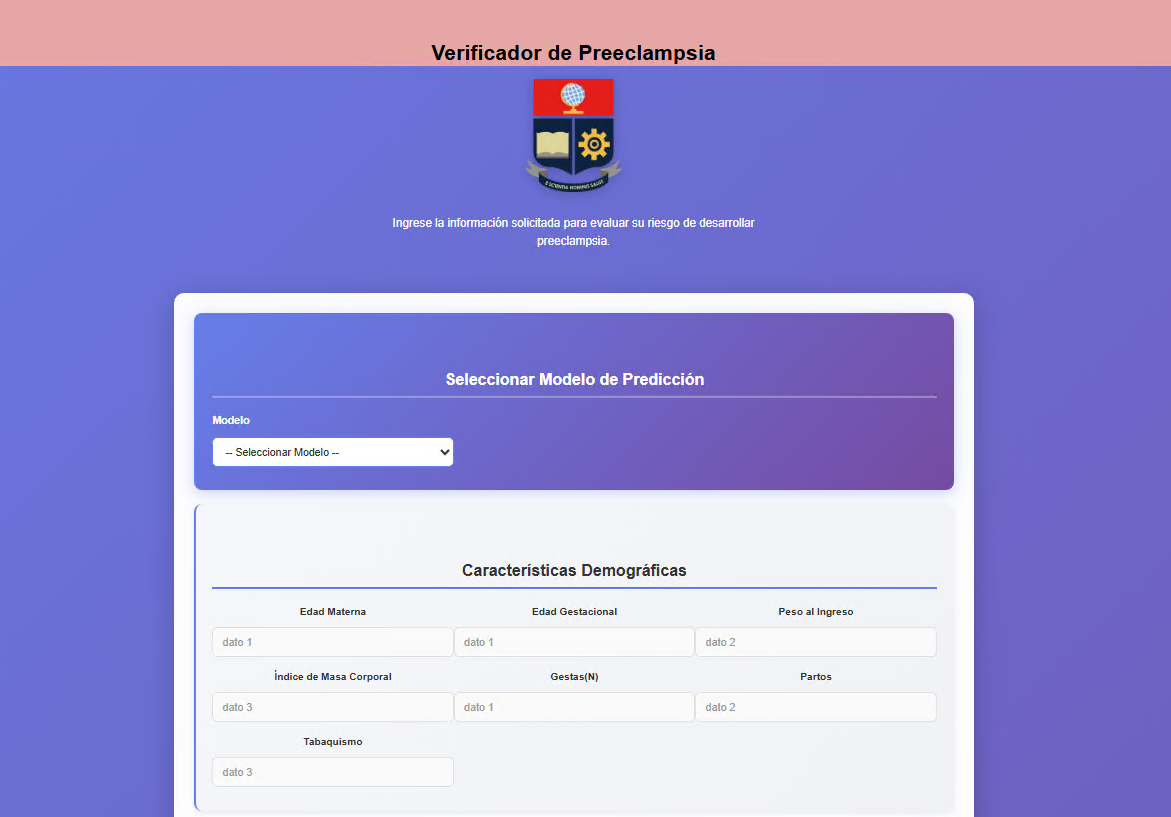
\includegraphics[width=0.48\fulllength]{figures/mlops/mlops_interface_demographic.png}}
\subfloat[\centering \label{fig:mlops-interface-b}]{
  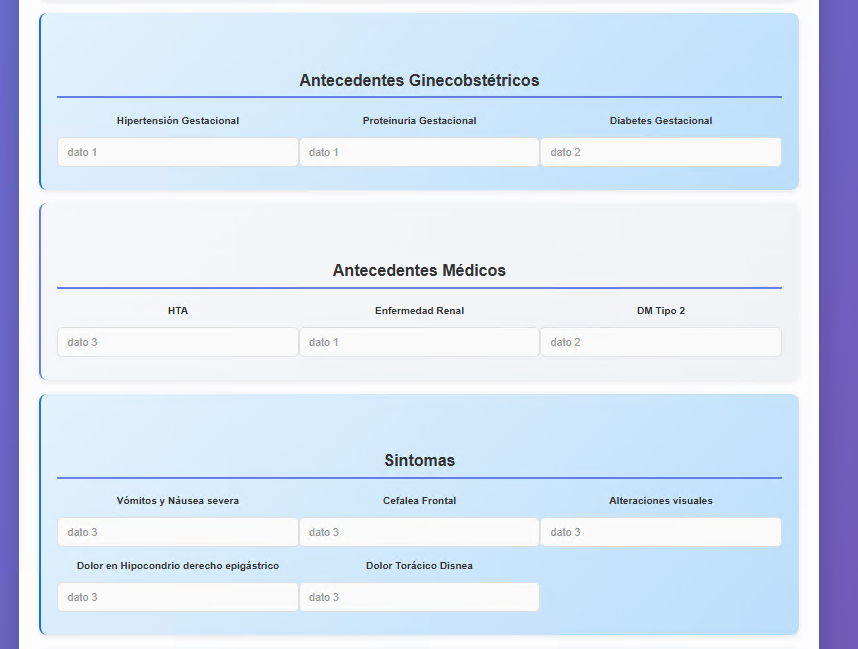
\includegraphics[width=0.48\fulllength]{figures/mlops/mlops_interface_clinical_history.png}}\\
\subfloat[\centering \label{fig:mlops-interface-c}]{
  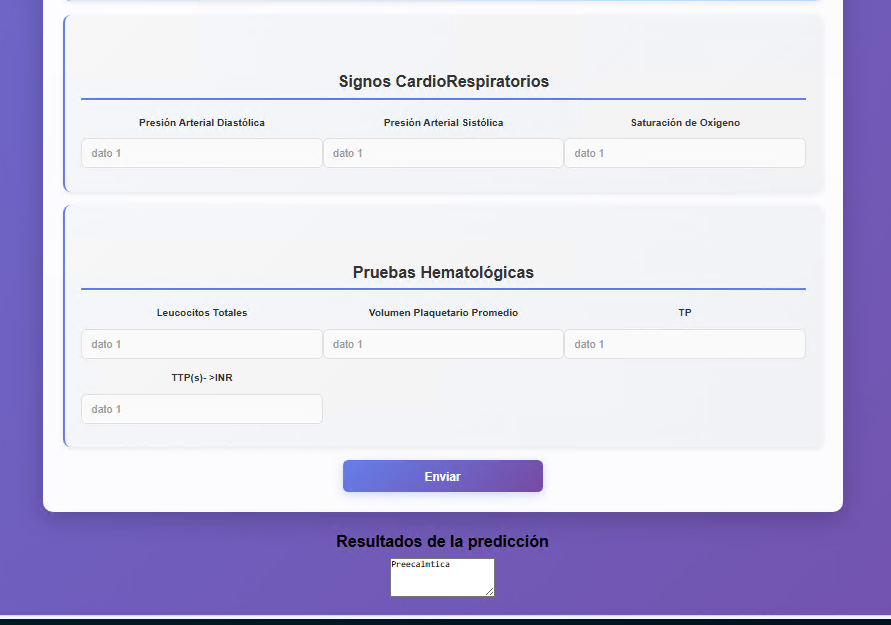
\includegraphics[width=0.48\fulllength]{figures/mlops/mlops_interface_signs_submit.png}}
\end{adjustwidth}
\caption{Web interface of the \textit{Verificador de Preeclampsia}
  system deployed at the Escuela Politécnica Nacional. (\textbf{a})
  Model selector and demographic input fields. (\textbf{b}) Clinical
  history and symptom input fields. (\textbf{c}) Cardiorespiratory
  and haematological input fields with the prediction results panel.  (\textbf{a})~Model selection and demographic characteristics
  section.  (\textbf{b}) Gyneco-obstetric history, medical history, and symptoms
  section.  (\textbf{c}) Cardiorespiratory signs, haematological tests, submission
  button, and prediction output
  panel.  \label{fig:mlops-interface}}
\end{figure}

%%%%%%%%%%%%%%%%%%%%%%%%%%%%%%%%%%%%%%%%%%
%\isPreprints{}{% This command is only used for ``preprints''.
\begin{adjustwidth}{-\extralength}{0cm}
%} % If the paper is ``preprints'', please uncomment this parenthesis.
%\printendnotes[custom] % Un-comment to print a list of endnotes

\reftitle{References}

% Please provide the correct journal abbreviation (e.g., according to the “List of Title Word Abbreviations” http://www.issn.org/services/online-services/access-to-the-ltwa/).
% Citations and References in Supplementary files are permitted provided that they also appear in the reference list here. 

%=====================================
% References, variant A: external bibliography
%=====================================
%\bibliography{bibliography.bib}
\begin{thebibliography}{999}

\bibitem[Vera-Ponce et~al.(2025)Vera-Ponce, Loayza-Castro, Ballena-Caicedo,
  Valladolid-Sandoval, Zuzunaga-Montoya, and Gutierrez
  De~Carrillo]{vera2025preeclampsia}
Vera-Ponce, V.J.; Loayza-Castro, J.A.; Ballena-Caicedo, J.;
  Valladolid-Sandoval, L.A.M.; Zuzunaga-Montoya, F.E.; Gutierrez De~Carrillo,
  C.I.
\newblock Global prevalence of preeclampsia, eclampsia, and HELLP syndrome: A
  systematic review and meta-analysis.
\newblock {\em Front. Reprod. Health} {\bf 2025}, {\em  7}, 1706009.
\newblock {\url{https://doi.org/10.3389/frph.2025.1706009}}.

\bibitem[{World Health Organization}(2025)]{who_2025_preeclampsia}
{World Health Organization}.
\newblock Pre-Eclampsia.   
\newblock WHO Fact Sheet. 2025.
\newblock Available online:
\url{https://www.who.int/news-room/fact-sheets/detail/pre-eclampsia}
{(accessed on 24 March 2026).} %MDPI: Please add the access date
                                %(format: Date Month Year), e.g.,
                                %accessed on 1 January
                                %2020. <<AUTHORS: added date>>

 

\bibitem[Brown et~al.(2018)Brown, Magee, Kenny, Karumanchi, McCarthy, Saito,
  Hall, Warren, Adoyi, and Ishaku]{brown2018isshp}
Brown, M.A.; Magee, L.A.; Kenny, L.C.; Karumanchi, S.A.; McCarthy, F.P.; Saito,
  S.; Hall, D.R.; Warren, C.E.; Adoyi, G.; Ishaku, S.
\newblock Hypertensive Disorders of Pregnancy.
\newblock {\em Hypertension} {\bf 2018}, {\em 72},~24--43.
%  \href{http://arxiv.org/abs/https://www.ahajournals.org/doi/pdf/10.1161/HYPERTENSIONAHA.117.10803}{{\normalfont
%  [https://www.ahajournals.org/doi/pdf/10.1161/HYPERTENSIONAHA.117.10803]}}.
\newblock {\url{https://doi.org/10.1161/HYPERTENSIONAHA.117.10803}}.

\bibitem[{Ministerio de Salud P\'ublica}(2016)]{msp_ecuador_hdp_2013}
{Ministerio de Salud P\'ublica}.
\newblock \emph{Trastornos Hipertensivos del Embarazo: Gu\'ia de Pr\'actica Cl\'inica
  (GPC)};  {Ministerio de Salud P\'ublica:} %MDPI: Newly added
                                %information. Please
                                %confirm. <<AUTHORS: we included an
                                %Ecuadorian Guide on the matter that
                                %is used at clinical level. We confirm
                                %it is a new information and they do
                                %have an ISBN but They do not have a
                                %doi because of the nature of the
                                %publication. The .bibtex entry
                                %contains the ISBN>> 
 Quito, Ecuador, {2016}.
\newblock   %MDPI: Please check if it should
                                %remove <<AUTHORS: Confirmed. We removed the unnecessary trailing text in this reference entry and retained only the required bibliographic information.>>


\bibitem[xin Li et~al.(2021)xin Li, ping Shen, Yang, zeng Cao, Du, da~Yu, ping
  Wang, and Wang]{LI2021102}
Li, Y.X.; Shen, X.P.; Yang, C.; Cao, Z.Z.; Du, R.; Yu, M.D.; Wang, J.P.; Wang, M.
\newblock Novelelectronic health records applied for prediction of
  pre-eclampsia: Machine-learning algorithms.
\newblock {\em Pregnancy Hypertens.} {\bf 2021}, {\em 26},~102--109.
\newblock {\url{https://doi.org/https://doi.org/10.1016/j.preghy.2021.10.006}}.

\bibitem[Mennickent et~al.(2023)Mennickent, Rodr\'iguez, Opazo, Riedel, Castro,
  Eriz-Salinas, Appel-Rubio, Aguayo, Damiano, Guzm\'an-Guti\'errez, and
  Araya]{mennickent_2023}
Mennickent, D.; Rodr\'iguez, A.; Opazo, M.C.; Riedel, C.A.; Castro, E.;
  Eriz-Salinas, A.; Appel-Rubio, J.; Aguayo, C.; Damiano, A.E.;
  Guzm\'an-Guti\'errez, E.;  et~al.
\newblock Machine learning applied in maternal and fetal health: A narrative
  review focused on pregnancy diseases and complications.
\newblock {\em Front. Endocrinol. (Lausanne)} {\bf 2023}, {\em 14}, 1130139.
\newblock {\url{https://doi.org/10.3389/fendo.2023.1130139}}.

\bibitem[Ranjbar et~al.(2024)Ranjbar, Montazeri, Ghamsari, Mehrnoush, Roozbeh,
  and Darsareh]{Darsareh2024}
Ranjbar, A.; Montazeri, F.; Ghamsari, S.R.; Mehrnoush, V.; Roozbeh, N.;
  Darsareh, F.
\newblock Machine learning models for predicting preeclampsia: A systematic
  review.
\newblock {\em BMC Pregnancy Childbirth} {\bf 2024}, {\em 24},~6.
\newblock {\url{https://doi.org/10.1186/s12884-023-06220-1}}.

\bibitem[Rahman et~al.(2023)Rahman, Lakulu, and Panessai]{Rahman2023}
Rahman, R.T.A.; Lakulu, M.M.; Panessai, I.Y.
\newblock Advancing Preeclampsia Prediction with Machine Learning: A
  Comprehensive Systematic Literature Review.
\newblock {\em Int. J. Intell. Syst. Appl. Eng.} {\bf 2023}, {\em 11},~13--23.

\bibitem[von Dadelszen et~al.(2011)von Dadelszen, Magee, Thabane, and
  et~al.]{fullpiers_2011}
von Dadelszen, P.; Payne, B.; Li, J.; Ansermino, J.M.; Pipkin, F.B.; Côté, A.M.; Douglas, M.J.; Gruslin, A.; Hutcheon, J.A.; Joseph, K.S.; et~al.
\newblock Prediction of adverse maternal outcomes in pre-eclampsia: Development
  and validation of the fullPIERS model.
\newblock {\em  Lancet} {\bf 2011}, {\em 377},~219--227.
\newblock {\url{https://doi.org/10.1016/S0140-6736(10)61351-7}}.

\bibitem[Cox(1958)]{cox1958logistic}
Cox, D.R.
\newblock The Regression Analysis of Binary Sequences.
\newblock {\em J. R. Stat. Soc. Ser. 
  (Methodol.)} {\bf 1958}, {\em 20},~215--232.
%  \href{http://arxiv.org/abs/https://academic.oup.com/jrsssb/article-pdf/20/2/215/49096552/jrsssb\_20\_2\_215.pdf}{{\normalfont
%  [https://academic.oup.com/jrsssb/article-pdf/20/2/215/49096552/jrsssb\_20\_2\_215.pdf]}}.
\newblock {\url{https://doi.org/10.1111/j.2517-6161.1958.tb00292.x}}.

\bibitem[Ke et~al.(2017)Ke, Meng, Finley, Wang, Chen, Ma, Ye, and
  Liu]{ke2017lightgbm}
Ke, G.; Meng, Q.; Finley, T.; Wang, T.; Chen, W.; Ma, W.; Ye, Q.; Liu, T.Y.
\newblock LightGBM: A Highly Efficient Gradient Boosting Decision Tree.
\newblock In \emph{Proceedings of the Advances in Neural Information Processing
  Systems}; Guyon, I., Luxburg, U.V., Bengio, S., Wallach, H., Fergus, R.,
  Vishwanathan, S., Garnett, R., Eds.; {Curran Associates, Inc.:
    Red Hook, NY, USA, } %MDPI: We are sorry but we could not find the
                         %required information about this
                         %entry. Please add the location of the
                         %publisher (city and country). <<AUTHORS: you
                         %can check the following to confirm the
                         %location https://dl.acm.org/doi/proceedings/10.5555/3294996>>
 2017; Volume~30.

\bibitem[Chen and Guestrin(2016)]{chen2016xgboost}
Chen, T.; Guestrin, C.
\newblock XGBoost: A Scalable Tree Boosting System.
\newblock In Proceedings of the  22nd ACM SIGKDD
  International Conference on Knowledge Discovery and Data Mining,
  {San Francisco, CA, USA,  13--17  August} %MDPI: Newly added
                                %information. Please confirm. Same
                                %with below highlight. <<AUTHORS: Confirmed. We added and verified the conference location and dates for this proceeding entry: San Francisco, CA, USA, 13--17 August 2016.>>
 2016; pp.
  785--794.
\newblock {\url{https://doi.org/10.1145/2939672.2939785}}.

\bibitem[Prokhorenkova et~al.(2018)Prokhorenkova, Gusev, Vorobev, Dorogush, and
  Gulin]{prokhorenkova2018catboost}
Prokhorenkova, L.; Gusev, G.; Vorobev, A.; Dorogush, A.V.; Gulin, A.
\newblock CatBoost: Unbiased boosting with categorical features.
\newblock In \emph{Proceedings of the Advances in Neural Information Processing
  Systems}; Bengio, S., Wallach, H., Larochelle, H., Grauman, K., Cesa-Bianchi,
  N., Garnett, R., Eds.; {Curran Associates, Inc.: Red Hook, NY,
    USA,} %MDPI: We are sorry but we could not find the required
          %information about this entry. Please add the location of
          %the publisher (city and country).<<AUTHORS: added the
          %information on the conference>>
  2018; Volume~31.

\bibitem[Rumelhart et~al.(1986)Rumelhart, Hinton, and
  Williams]{rumelhart1986backprop}
Rumelhart, D.E.; Hinton, G.E.; Williams, R.J.
\newblock Learning representations by back-propagating errors.
\newblock {\em Nature} {\bf 1986}, {\em 323},~533--536.
\newblock {\url{https://doi.org/10.1038/323533a0}}.

\bibitem[Breiman(2001)]{breiman2001randomforest}
Breiman, L.
\newblock Random Forests.
\newblock {\em Mach. Learn.} {\bf 2001}, {\em 45},~5--32.
\newblock {\url{https://doi.org/10.1023/A:1010933404324}}.

\bibitem[Marin et~al.(2019)Marin, Pavaloiu, Marian, Racovita, and
  Goga]{marin2019}
Marin, I.; Pavaloiu, B.I.; Marian, C.V.; Racovita, V.; Goga, N.
\newblock Early Detection of Preeclampsia based on a Machine Learning Approach.
\newblock In \emph{Proceedings of the 2019 E-Health and Bioengineering Conference
  (EHB)}; IEEE: {New York, NY, USA,} 
  2019; pp. 1--4.
\newblock {\url{https://doi.org/10.1109/ehb47216.2019.8970025}}.

\bibitem[Maric et~al.(2022)Maric, Contrepois, Moufarrej, Stelzer, Feyaerts,
  Han, Tang, Stanley, Wong, Traber, Ellenberger, Chang, Fallahzadeh, Nassar,
  Becker, Xenochristou, Espinosa, Francesco, Ghaemi, Costello, Culos, Ling,
  Sylvester, Darmstadt, Winn, Shaw, Relman, Quake, Angst, Snyder, Stevenson,
  Gaudilliere, and Aghaeepour]{mari__2022}
Maric, I.; Contrepois, K.; Moufarrej, M.N.; Stelzer, I.A.; Feyaerts, D.; Han,
  X.; Tang, A.; Stanley, N.; Wong, R.J.; Traber, G.M.;  et~al.
\newblock Early prediction and longitudinal modeling of preeclampsia from
  multiomics.
\newblock {\em Patterns} {\bf 2022}, {\em 3},~100655.
\newblock {\url{https://doi.org/10.1016/j.patter.2022.100655}}.

\bibitem[Mari\'c et~al.(2020)Mari\'c, Tsur, Aghaeepour, Montanari, Stevenson,
  Shaw, and Winn]{mari__2020}
Mari\'c, I.; Tsur, A.; Aghaeepour, N.; Montanari, A.; Stevenson, D.K.; Shaw,
  G.M.; Winn, V.D.
\newblock Early prediction of preeclampsia via machine learning.
\newblock {\em Am. J. Obstet. Gynecol. MFM} {\bf 2020}, {\em 2},~100100.
\newblock {\url{https://doi.org/10.1016/j.ajogmf.2020.100100}}.

\bibitem[Long et~al.(2024)Long, Flicker, Vishnia, Wright, Francis, King,
  Gilgannon, Rastegar, Gupta, Siva, Nehme, and Kawakita]{long2025fullpiers}
Long, D.; Flicker, K.; Vishnia, M.; Wright, M.; Francis, M.; King, K.S.;
  Gilgannon, L.; Rastegar, A.; Gupta, N.; Siva, R.K.;  et~al.
\newblock External Validation of the fullPIERS Risk Prediction Model in a U.S.
  Cohort of Individuals with Preeclampsia.
\newblock {\em Am. J. Perinatol.} {\bf 2024}, {\em
  42},~1035--1042.
\newblock {\url{https://doi.org/10.1055/a-2452-8220}}.

\bibitem[{do Valle Teichmann} et~al.(2025){do Valle Teichmann}, Naibo, {da Cruz
  Rodrigues}, {de Matos}, {de Almeida Martins Costa}, and
  Ramos]{teichmann2025fullpiers}
{do Valle Teichmann}, P.; Naibo, R.A.; {da Cruz Rodrigues}, M.A.; {de Matos},
  M.W.; {de Almeida Martins Costa}, S.H.; Ramos, J.G.L.
\newblock Validation of the fullPIERS model in a tertiary hospital in southern
  Brazil.
\newblock {\em Pregnancy Hypertens.} {\bf 2025}, {\em 41},~101237.
\newblock {\url{https://doi.org/10.1016/j.preghy.2025.101237}}.

\bibitem[Moyene et~al.(2025)Moyene, Beya, Nyota, Masidi, Kilembo, Natuhoyila,
  Verdonck, and Spitz]{elongi2025fullpiers}
Moyene, J.P.E.; Beya, D.T.; Nyota, P.K.; Masidi, J.M.; Kilembo, E.L.;
  Natuhoyila, A.N.; Verdonck, F.; Spitz, B.
\newblock Evaluation of the Performance of fullPIERS (Preeclampsia Integrated
  Estimate of Risk Scoring) in Predicting Maternal-Fetal Complications in
  Congolese Women with Preeclampsia.
\newblock {\em J. Obstet. Gynaecol. Can.} {\bf 2025}, {\em
  47}, 102812.
\newblock {\url{https://doi.org/10.1016/j.jogc.2025.102812}}.

\bibitem[Millman et~al.(2011)Millman, Payne, Qu, {Joanne Douglas}, Hutcheon,
  Lee, Magee, Walley, and {von Dadelszen}]{millman2011spo2}
Millman, A.L.; Payne, B.; Qu, Z.; {Joanne Douglas}, M.; Hutcheon, J.A.; Lee,
  T.; Magee, L.A.; Walley, K.R.; {von Dadelszen}, P.
\newblock Oxygen Saturation as a Predictor of Adverse Maternal Outcomes in
  Women with Preeclampsia.
\newblock {\em J. Obstet. Gynaecol. Can.} {\bf 2011}, {\em
  33},~705--714.
\newblock {\url{https://doi.org/10.1016/S1701-2163(16)34955-6}}.

\bibitem[{Amazon Web Services}(2026)]{aws_sagemaker_canvas_docs}
{Amazon Web Services}.
\newblock What Is Amazon SageMaker Canvas?  2026.
\newblock Available online: \url{https://docs.aws.amazon.com/sagemaker/latest/dg/canvas.html} {(accessed on 5 April 2026).} 

%\newblock AWS documentation, accessed 2026-04-05.

\bibitem[Erickson et~al.(2020)Erickson, Mueller, Shirkov, Zhang, Larroy, Li,
  and Smola]{agtabular2020}
Erickson, N.; Mueller, J.; Shirkov, A.; Zhang, H.; Larroy, P.; Li, M.; Smola,
  A.
\newblock {AutoGluon-Tabular}: Robust and Accurate {AutoML} for Structured
  Data.
\newblock {\em arXiv} {\bf 2020}, arXiv:2003.06505.
 % \href{http://arxiv.org/abs/2003.06505}{{\normalfont [2003.06505]}}.

\bibitem[Caruana et~al.(2004)Caruana, Niculescu-Mizil, Crew, and
  Ksikes]{caruana2004ensemble}
Caruana, R.; Niculescu-Mizil, A.; Crew, G.; Ksikes, A.
\newblock Ensemble Selection from Libraries of Models.
\newblock In Proceedings of the  21st International
  Conference on Machine Learning (ICML), Banff, AB, Canada,  {4--8 July} %<<AUTHORS: Confirmed. We also verified and kept the conference date information in this highlighted proceeding entry.>>
 2004; p.~18.
\newblock {\url{https://doi.org/10.1145/1015330.1015432}}.

\bibitem[Bergstra and Bengio(2012)]{bergstra2012random}
Bergstra, J.; Bengio, Y.
\newblock Random Search for Hyper-Parameter Optimization.
\newblock {\em J. Mach. Learn. Res.} {\bf 2012}, {\em
  13},~281--305.

\bibitem[Pedregosa et~al.(2011)Pedregosa, Varoquaux, Gramfort, Michel, Thirion,
  Grisel, Blondel, Prettenhofer, Weiss, Dubourg, Vanderplas, Passos,
  Cournapeau, Brucher, Perrot, and Duchesnay]{sklearn-api}
Pedregosa, F.; Varoquaux, G.; Gramfort, A.; Michel, V.; Thirion, B.; Grisel,
  O.; Blondel, M.; Prettenhofer, P.; Weiss, R.; Dubourg, V.;  et~al.
\newblock Scikit-learn: Machine Learning in {P}ython.
\newblock {\em J. Mach. Learn. Res.} {\bf 2011}, {\em
  12},~2825--2830.

\bibitem[Fawcett(2006)]{fawcett2006roc}
Fawcett, T.
\newblock An introduction to ROC analysis.
\newblock {\em Pattern Recognit. Lett.} {\bf 2006}, {\em 27},~861--874.
\newblock {\url{https://doi.org/10.1016/j.patrec.2005.10.010}}.

\bibitem[Sokolova and Lapalme(2009)]{sokolova2009systematic}
Sokolova, M.; Lapalme, G.
\newblock A systematic analysis of performance measures for classification
  tasks.
\newblock {\em Inf. Process. Manag.} {\bf 2009}, {\em
  45},~427--437.
\newblock {\url{https://doi.org/10.1016/j.ipm.2009.03.002}}.

\bibitem[Powers(2020)]{powers2011evaluation}
Powers, D.M.W.
\newblock Evaluation: From precision, recall and F-measure to ROC,
  informedness, markedness and correlation.  \emph{arXiv} \textbf{2020}. arXiv:2010.16061
  %\href{http://arxiv.org/abs/2010.16061}{{\normalfont
%  [arXiv:cs.LG/2010.16061]}}.

\bibitem[Lundberg and Lee(2017)]{lundberg2017shap}
Lundberg, S.M.; Lee, S.I.
\newblock A Unified Approach to Interpreting Model Predictions.
\newblock In \emph{Proceedings of the Advances in Neural Information Processing
  Systems}; Guyon, I., Luxburg, U.V., Bengio, S., Wallach, H., Fergus, R.,
  Vishwanathan, S., Garnett, R., Eds.; {Curran Associates, Inc.: Red Hook, NY,
    USA,} %MDPI: We are sorry but we could not find the required
          %information about this entry. Please add the location of
          %the publisher (city and country). <<AUTHORS: added>>
  2017; Volume~30,
  pp. 4765--4774.

\bibitem[Li et~al.(2022)Li, Wang, Vieira, Zheutlin, Ru, Schadt, Wang,
  Copperman, Stone, Gross, Kao, Lau, Dolan, Schadt, and
  Li]{liu_pregnancy_trajectories_2022}
Li, S.; Wang, Z.; Vieira, L.A.; Zheutlin, A.B.; Ru, B.; Schadt, E.; Wang, P.;
  Copperman, A.B.; Stone, J.L.; Gross, S.J.;  et~al.
\newblock Improving preeclampsia risk prediction by modeling pregnancy
  trajectories from routinely collected electronic medical record data.
\newblock {\em NPJ Digit. Med.} {\bf 2022}, {\em 5},~68.
\newblock {\url{https://doi.org/10.1038/s41746-022-00612-x}}.

\bibitem[Li et~al.(2024)Li, Xu, Wang, Wang, Tang, Duan, Zhao, Zheng, and
  Hu]{zeng_preeclampsia_ml_china_2024}
Li, T.; Xu, M.; Wang, Y.; Wang, Y.; Tang, H.; Duan, H.; Zhao, G.; Zheng, M.;
  Hu, Y.
\newblock Prediction model of preeclampsia using machine learning based
  methods: A population based cohort study in China.
\newblock {\em Front. Endocrinol.} {\bf 2024}, {\em  15}, 1345573.
\newblock {\url{https://doi.org/10.3389/fendo.2024.1345573}}.

\bibitem[Jain et~al.(2025)Jain, Saxena, Joshi, Gorbachenko, and
  Kuzmin]{advancing_ml_preeclampsia_2025}
Jain, P.; Saxena, J.; Joshi, A.; Gorbachenko, V.; Kuzmin, A.
\newblock Advancing machine learning tools for early prediction and clinical
  diagnosis of pre-eclampsia.
\newblock {\em Pregnancy Hypertens.} {\bf 2025}, {\em 42},~101269.
\newblock {\url{https://doi.org/10.1016/j.preghy.2025.101269}}.

\bibitem[Liu et~al.(2026)Liu, Zhu, Zong, Chen, Zhang, and
  Wang]{jmijr_ml_pe_review_2026}
Liu, L.; Zhu, Q.; Zong, Y.; Chen, X.; Zhang, W.; Wang, J.
\newblock Machine Learning Prediction Models for Preeclampsia: Systematic
  Review and Meta-Analysis.
\newblock {\em J. Med. Internet Res.} {\bf 2026}, {\em 28},~e78714.
\newblock {\url{https://doi.org/10.2196/78714}}.

\bibitem[{conda-forge community}(2024)]{miniforge2021}
{Conda-Forge Community}.
\newblock {\emph{mamba}, Version 2.4.0; Software for Package and Environment
  Management; Zenodo: Geneva, Switzerland, 2024.} %MDPI: We are
                                %sorry but we could not find the
                                %required information about this
                                %entry. Please provide more
                                %information about this article,
                                %whether it is a book (please provide
                                %the name and location of the
                                %publisher); online resource (please
                                %provide the URL of the website and
                                %the date it was accessed (Date Month
                                %Year)); or journal article (please
                                %provide the name of the journal, the
                                %year and volume in which it was
                                %published, and the page
                                %number). Please refer to
                                %https://www.mdpi.com/authors/references
                                %for full reference formatting
                                %guides. <<AUTHORS: Confirmed. This software deposit is archived on Zenodo (doi: 10.5281/zenodo.4774216). We reformatted it following the MDPI software-citation format: Title, version; comments; Publisher: Place, Year, listing Zenodo (Geneva, Switzerland) as the publisher.>>
% FORMAT: Creator (if available). Title, version; comments; Publisher: Place, Year.
%   Creator   = {conda-forge community}  [bibitem author line]
%   Title     = mamba
%   version   = Version 2.4.0
%   comments  = Software for Package and Environment Management
%   Publisher = Zenodo  [hosts the archived software deposit; doi: 10.5281/zenodo.4774216]
%   Place     = Geneva, Switzerland
%   Year      = 2024
%   NOTE: Creator =/= Publisher (developer vs. archive host)

\bibitem[{Anaconda, Inc.}(2020)]{anaconda2020package}
{Anaconda, Inc.}
\newblock {\emph{Anaconda Software Distribution}, Version 26.3.2; Computer
  Software; Anaconda, Inc.: Austin, TX, USA, 2020.} %MDPI: We are
                                %sorry but we could not find the
                                %required information about this
                                %entry. Please add the name of the
                                %publisher and their
                                %location. <<AUTHORS: Confirmed. We reformatted this entry following the MDPI software-citation format: Title, version; comments; Publisher: Place, Year. We merged it into a single statement and added the publisher name and location (Anaconda, Inc.: Austin, TX, USA) as requested.>>
% FORMAT: Creator (if available). Title, version; comments; Publisher: Place, Year.
%   Creator   = {Anaconda, Inc.}  [bibitem author line]
%   Title     = Anaconda Software Distribution
%   version   = Version 26.3.2
%   comments  = Computer Software
%   Publisher = Anaconda, Inc.  [same org as creator -- valid per MDPI Mathematica example]
%   Place     = Austin, TX, USA
%   Year      = 2020


\bibitem[{Python Packaging Authority}(2026)]{pip_pypa}
{Python Packaging Authority}.
\newblock {\emph{pip}, Version 26.0.1; Software for Python Package
  Management; Python Packaging Authority: Online, 2026.} %MDPI: Please add the access date (format: Date Month Year),
        %e.g., accessed on 1 January 2020. <<AUTHORS: Confirmed. This is a software entry, not a website citation. We reformatted it following the MDPI software-citation format: Title, version; comments; Publisher: Place, Year. Since the Python Packaging Authority has no fixed physical address, we used "Online" as the place of publication.>>
% FORMAT: Creator (if available). Title, version; comments; Publisher: Place, Year.
%   Creator   = {Python Packaging Authority}  [bibitem author line]
%   Title     = pip
%   version   = Version 26.0.1
%   comments  = Software for Python Package Management
%   Publisher = Python Packaging Authority  [same org as creator -- valid per MDPI Mathematica example]
%   Place     = Online  [PyPA has no registered physical address]
%   Year      = 2026


\bibitem[Zaharia et~al.(2018)Zaharia, Chen, Davidson, Ghodsi, Hong, Konwinski,
  Murching, Nykodym, Ogilvie, Parkhe, et~al.]{mlflow_2018}
Zaharia, M.; Chen, A.; Davidson, A.; Ghodsi, A.; Hong, S.A.; Konwinski, A.;
  Murching, S.; Nykodym, T.; Ogilvie, P.; Parkhe, M.;  et~al.
\newblock Accelerating the Machine Learning Lifecycle with {MLflow}.
\newblock {\em IEEE Data Eng. Bull.} {\bf 2018}, {\em 41},~39--45.

\end{thebibliography}

%=====================================
% references, variant B: internal bibliography
%=====================================

% ACS format
% \begin{thebibliography}{999}
% % Reference 1
% \bibitem{ref-journal}
% Author~1, T. The title of the cited article. {\em Journal Abbreviation} {\bf 2008}, {\em 10}, 142--149.
% % Reference 2
% \bibitem{ref-book1}
% Author~2, L. The title of the cited contribution. In {\em The Book Title}; Editor 1, F., Editor 2, A., Eds.; Publishing House: City, Country, 2007; pp. 32--58.
% % Reference 3
% \bibitem{ref-book2}
% Author 1, A.; Author 2, B. \textit{Book Title}, 3rd ed.; Publisher: Publisher Location, Country, 2008; pp. 154--196.
% % Reference 4
% \bibitem{ref-unpublish}
% Author 1, A.B.; Author 2, C. Title of Unpublished Work. \textit{Abbreviated Journal Name} year, \textit{phrase indicating stage of publication (submitted; accepted; in press)}.
% % Reference 5
% \bibitem{ref-url}
% Title of Site. Available online: URL (accessed on Day Month Year).
% % Reference 6
% \bibitem{ref-proceeding}
% Author 1, A.B.; Author 2, C.D.; Author 3, E.F. Title of presentation. In Proceedings of the Name of the Conference, Location of Conference, Country, Date of Conference (Day Month Year); Abstract Number (optional), Pagination (optional).
% % Reference 7
% \bibitem{ref-thesis}
% Author 1, A.B. Title of Thesis. Level of Thesis, Degree-Granting University, Location of University, Date of Completion.
% \end{thebibliography}

% If authors have biography, please use the format below
%\section*{Short Biography of Authors}
%\bio
%{\raisebox{-0.35cm}{\includegraphics[width=3.5cm,height=5.3cm,clip,keepaspectratio]{Definitions/author1.pdf}}}
%{\textbf{Firstname Lastname} Biography of first author}
%
%\bio
%{\raisebox{-0.35cm}{\includegraphics[width=3.5cm,height=5.3cm,clip,keepaspectratio]{Definitions/author2.jpg}}}
%{\textbf{Firstname Lastname} Biography of second author}

% For the MDPI journals use author-date citation, please follow the formatting guidelines on http://www.mdpi.com/authors/references
% To cite two works by the same author: \citeauthor{ref-journal-1a} (\citeyear{ref-journal-1a}, \citeyear{ref-journal-1b}). This produces: Whittaker (1967, 1975)
% To cite two works by the same author with specific pages: \citeauthor{ref-journal-3a} (\citeyear{ref-journal-3a}, p. 328; \citeyear{ref-journal-3b}, p.475). This produces: Wong (1999, p. 328; 2000, p. 475)

%%%%%%%%%%%%%%%%%%%%%%%%%%%%%%%%%%%%%%%%%%
%% for journal Sci
%\reviewreports{\\
%Reviewer 1 comments and authors’ response\\
%Reviewer 2 comments and authors’ response\\
%Reviewer 3 comments and authors’ response
%}
%%%%%%%%%%%%%%%%%%%%%%%%%%%%%%%%%%%%%%%%%%
\PublishersNote{}
%\isPreprints{}{% This command is only used for ``preprints''.
\end{adjustwidth}
%} % If the paper is ``preprints'', please uncomment this parenthesis.
\end{document}


%%% Local Variables:
%%% mode: LaTeX
%%% TeX-master: t
%%% End:
